\documentclass[12pt, letterpaper]{report}   % Single-sided printing for the library

% TOGGLE ON TO SEE PAGE MARGINS -- useful to check that your figures and tables don't go over the specified margins - HG 2018
% \usepackage[showframe]{geometry}

\usepackage[bf]{caption} % Make nice captions with bold "Figure..." and "Table..."
\setcaptionmargin{0.5in}
%package for the bu thesis format -- most commonly-used packages added in the style file by HG 2018
\usepackage{bu_math_thesis}

% \usepackage{titletoc}
% \usepackage{capt-of}
\usepackage{tocloft}
\usepackage{xpatch}

% \usepackage{hyperref}

% Just in case we're not using hyperref
% \providecommand{\phantomsection}{}

% Generate the separate list of commands for appendix figures and tables
\newcommand{\listofappendixfiguresname}{List of Figures in Appendices}
\newlistof{appendixfigures}{apf}{\listofappendixfiguresname}
\newcommand{\listofappendixtablesname}{List of Tables in Appendix}
\newlistof{appendixtables}{apt}{\listofappendixtablesname}

\renewcommand{\cftafterapftitle}{\addcontentsline{toc}{chapter}{\listofappendixfiguresname}}
\renewcommand{\cftafterapttitle}{\phantomsection\addcontentsline{toc}{chapter}{\listofappendixtablesname}}

\xpretocmd{\listofappendixfigures}{\clearpage}{}{}
\xpretocmd{\listofappendixtables}{\clearpage}{}{}


\makeatletter
\xapptocmd{\appendix}{%
  \write\@auxout{%
    \string\let\string\latex@tf@lof\string\tf@lof% Store the original `\tf@lof` file handle
    \string\let\string\tf@lof\string\tf@apf% 
    \string\let\string\latex@tf@lof\string\tf@lot% Store the original `\tf@lot` file handle
    \string\let\string\tf@lot\string\tf@apt% 
  }%
}{}{}
\makeatother


\graphicspath{{figures/}{tables/}}

%%%%%%%%%%%%%%%%%%%%%%%%%%%%%%%%%%%%%%%%%%%%%%%%%%%%%%%%%%%%%%%%%%%%%%%%%%
%define the frequent formulas shorthands for typing -- note that these do not appear as the function in "Rich Text" format in Overleaf, but rather as the "\shorthand"
%Packages
% \usepackage{lipsum}
\usepackage[T1]{fontenc}
\usepackage{fourier} 
\usepackage[english]{babel} 
\usepackage{amsmath,amsfonts} 
\usepackage{amsthm} 
\usepackage{color}   %May be necessary if you want to color links
\usepackage{hyperref}
\usepackage{lscape}
\usepackage{geometry}
\usepackage{amsmath}
\usepackage{algorithm}
\usepackage{algorithmic}
\usepackage{amssymb}
\usepackage{amsfonts}
\usepackage{times}
\usepackage{bm}
\usepackage{ stmaryrd }
\SetSymbolFont{stmry}{bold}{U}{stmry}{m}{n}
\usepackage{ amssymb }
\usepackage{ textcomp }
\usepackage[normalem]{ulem}
% For derivation rules
\usepackage{mathpartir}
\usepackage{color}
\usepackage{a4wide}
\usepackage{caption}
\usepackage{subcaption}
\usepackage{mathpartir}
\usepackage{amsmath,amsfonts}
\usepackage{ amssymb }
\usepackage{color}
\usepackage{algorithm}
\usepackage{algorithmic}
\usepackage{microtype}
\usepackage{eucal}
\usepackage{url}
\usepackage{tikz}
\usepackage{xspace}
\usepackage{array}
\usepackage{listings}
\usepackage{import}

\usetikzlibrary{shapes.geometric}
\usetikzlibrary{arrows.meta,arrows}
\usetikzlibrary{decorations.text}
% % % % 

%%%% Extra packages
\usepackage[T1]{fontenc}
\usepackage[latin9]{inputenc}
\usepackage{amsmath}
\usepackage{amssymb}
\usepackage{cancel}

%%%%%%%%%%%%%%%%%%%%%%%%%%%%%% User specified LaTeX commands.
% \usepackage{typesetting/latex8}
% \usepackage{times}
% \usepackage{color}
% \usepackage{epsfig}
% \usepackage{graphicx}
% \usepackage{graphics}
% \usepackage{amsmath, nicefrac}
% \usepackage{amssymb, amsthm}
% \usepackage{wrapfig}
% \usepackage{algorithm, algorithmic}
% \usepackage{setspace}
% \usepackage{caption}
% \usepackage{float}
% \usepackage{afterpage}
% % \usepackage{typesetting/abstract}
% \usepackage{tabularx}
% \usepackage{booktabs}
% \usepackage{calc}
% \usepackage{multirow}
% \usepackage{longtable}
% \usepackage{footnote}
% \usepackage{threeparttable}
% \usepackage{colortbl}
% % \usepackage{tweaklist}
% \usepackage{fancyhdr}
% \usepackage[retainorgcmds]{IEEEtrantools}
% \usepackage{floatflt}
% \usepackage{xspace}

% \usepackage{endnotes}
% \usepackage{paralist}
% % \usepackage{typesetting/shortcuts}
% \usepackage{tabulary}
% \usepackage{mdwlist}
% \usepackage{listings}
% \usepackage{balance}
% \usepackage{url}
% \usepackage{parskip}
% \usepackage{textcomp}
% \usepackage{subcaption}

% \usepackage{epstopdf}
% \usepackage{fancyvrb}

% \makeatletter

\usepackage{xargs}
\usepackage{cleveref}
\newif\ifextra
\extratrue 


\newcommand{\lagin}{\ensuremath{\lambda_{1}}}
\newcommand{\lagout}{\ensuremath{\lambda_{2}}}

%%%%%%%%%%%%%%%%%%%%%%%%%%%%%%%%%%%%%%%%%%%%%%%%%%%%%%%%%%%%%%%%%%%%%%%%%%
\begin{document}
%%%%%%%%%%%%%%%%%%%%%%%%%%%%%%%%%%%%%%%%%%%%%%%%%%%%%%%%%%%%%%%%%%%%%%%%%%
% Setup commands for the bu thesis style file

\title{Program-based Analysis for Quantitative Properties}
\author{Jiawen Liu}

% Type of document prepared for this degree:
%   2 = Doctor of Philosophy dissertation.
%   4 = Doctoral Dissertation Prospectus
\degree=2

% List your bachelors degree before your masters - HG 2018
\prevdegrees{
B.A. in Department of Information Science, Central University of Economics and Finance, 2017\\ 
% MS in Computer Science, University at Buffalo, 2016
}
\department{Department of Computer Science}
\university{Boston University}
\faculty{Graduate School of Arts and Sciences}

% Degree year is the year the diploma is expected, and defense year is the year the dissertation is written up and defended. Often, these will be the same, except for January graduation, when your defense will be in the fall of year X, and your graduation will be in January of year X+1
\defenseyear{2023}
\degreeyear{2023}

% For each reader, specify appropriate label {First, second, third}, then name, then title. Warning: If you have more than five readers you are out of luck, because it will overflow to a new page. Sometimes you may wish to put part of the title in with the name
% Do NOT put the chair on your approval page - HG 2018
\reader{First}{Marco Gaboardi, Ph.D.}{Associate Professor, Computer Science}
\reader{Second}{ }{}
\reader{Third}{Assaf Kfoury, Ph.D.}{Professor, Computer Science}
\reader{Fourth}{ }{}
% \reader{Fifth}{Deepak Garg, Ph.D.}{Associate Professor, MPI-SWS}
% The Major Professor is the same as the first reader, but must be specified again for the abstract page
% Just copy and paste the same information
\majorprof{Marco Gaboardi}{Associate Professor of Computer Science}


%%%%%%%%%%%%%%%%%%%%%%%%%%%%%%%%%%%%%%%%%%%%%%%%%%%%%%%%%%%%%%%%%%%%%
% other set up commands which are a good idea

%the bottom margins should be "as close as possible" to 1 inch, so allowdisplaybreaks is a good idea for theses with a lot of equations
\allowdisplaybreaks


%%%%%%%%%%%%%%%%%%%%%%%%%%%%%%%%%%%%%%%%%%%%%%%%%%%%%%%%%%%%%%%%%%%%%
%                       PRELIMINARY PAGES
% According to the BU guide the preliminary pages consist of: title, copyright (optional), approval,  acknowledgments (opt.), abstract, preface (opt.), Table of contents, List of tables (if any), List of illustrations (if any). The \tableofcontents, \listoffigures, and \listoftables commands can be used in the appropriate places. For other things like preface, do it manually with something like \newpage\section*{Preface}.

%%%%%%%%%%%%%%%%%%%%%%%%%%%%%%%%%%%%%%%%%%%%%%%%%%%%%%%%%%%%%%%%%%%%
% This is an additional page (do not hand it in at the library) to print boxed-in title, author and degree statement so that they are visible through the opening in BU covers used for reports. This makes a nicely bound copy.

%\buecethesistitleboxpage

%%%%%%%%%%%%%%%%%%%%%%%%%%%%%%%%%%%%%%%%%%%%%%%%%%%%%%%%%%%%%%%%%%%%
%%%% TITLE PAGE 
% Make the titlepage based on the above information.  If you need something special and can't use the standard form, you can specify the exact text of the titlepage yourself.  Put it in a titlepage environment and leave blank lines where you want vertical space. The spaces will be adjusted to fill the entire page.
\maketitle

%%%%%%%%%%%%%%%%%%%%%%%%%%%%%%%%%%%%%%%%%%%%%%%%%%%%%%%%%%%%%%%%%%%%
%%%% COPYRIGHT PAGE 
% The copyright page is blank except for the notice at the bottom. You must provide your name in capitals.
\copyrightpage

%%%%%%%%%%%%%%%%%%%%%%%%%%%%%%%%%%%%%%%%%%%%%%%%%%%%%%%%%%%%%%%%%%%%
%%%% APPROVAL PAGE 
% Now include the approval page based on the readers information
\approvalpage

%%%%%%%%%%%%%%%%%%%%%%%%%%%%%%%%%%%%%%%%%%%%%%%%%%%%%%%%%%%%%%%%%%%%
%%%% DEDICATION			 
\addcontentsline{toc}{chapter}{Dedication}
\section*{Dedication}
\begin{flushright}
This dissertation is dedicated to \\
my loving grandfather \\ Zhaosheng Jin \\ \& \\ my dear grandmother \\ Dongju Gao
\end{flushright}


%%%%%%%%%%%%%%%%%%%%%%%%%%%%%%%%%%%%%%%%%%%%%%%%%%%%%%%%%%%%%%%%%%%%
%%%% ACKNOWLEDGEMENTS	 
\newpage
\addcontentsline{toc}{chapter}{Acknowledgements}
\section*{Acknowledgments}

I would like to first express my sincerest thanks to Boston University, 
it is a great experience to study, do research, and enjoy my life here. 
I am so lucky that I made my decision to transfer to Boston University during the summer of 2019. 
I like the seminars, like the classes, like my colleagues here, like the discussion about logic, type systems. 

I have been at BU for more than two years. 
Before that, I stayed at Buffalo for three years. 
Reviewing my path to Ph.D., so many people have helped me. 
In particular, I would like to say thank you so much to my advisor, Professor Marco Gaboardi. 
Thanks for your being an amazing advisor, for your bringing me to BU, for encouraging me to attend conferences, for providing great opportunities to collaborate with great researchers, for teaching me how to become a better human being! 
I am so fortunate that I can work with Marco for these years.

I want to thank my committee members. 
Great thanks to Professor Assaf Kfoury for your kindness in being the chair of my committee.

I would like to thank all my colleagues at Boston University as well as at the University at Buffalo. 
Thanks to Professor Lukasz Ziarek for his help at Buffalo. 
Thanks to all my collaborators in these works in the dissertation.

Last, but by no means least, I want to thank my grandmother Xiuqin Yang, for your support in pursuing my Ph.D. 
I am also thankful to my family members, my father Hui Liu, my mother Yahong Hu and my brother Hu Liu.  
Thanks to my lovely kitty Taro for his company. 



%%%%%%%%%%%%%%%%%%%%%%%%%%%%%%%%%%%%%%%%%%%%%%%%%%%%%%%%%%%%%%%%%%%%
%%%% ABSTRACT		 
\newpage
\addcontentsline{toc}{chapter}{Abstract}
Data analyses are usually designed to identify some property of the population from which the data are drawn, 
generalizing beyond the specific data sample. For this reason, data analyses are often designed in a way that guarantees that they produce a low generalization error.
 That is, they are designed so that the result of a data analysis run on sample 
 data does not differ too much from the result one would achieve by running the analysis over the entire population. 
 
 An adaptive data analysis can be seen as a process composed of multiple queries interrogating some data, where the choice of which query to run next may rely on the results of previous queries. 
 The generalization error of individual query/analysis can be controlled by using an array of well-established statistical techniques.
 However, when queries are arbitrarily composed, the different errors can propagate through the chain of different queries and bring high generalization errors. 
 To address this issue, data analysts are designing several techniques that not only guarantee bounds on the generalization errors of single queries, but also guarantee bounds on the generalization error of the composed analyses. 
 The choice of which of these techniques to use, 
 often depends on the chain of queries that an adaptive data analysis can generate.
 Specifically, the total number of queries and the depth of the chain of queries is of great significance 
 to guarantee the generalization error, 
 when the composed data analyses are adaptive. 
 So in order to give a precise guarantee of generalization error
 for the program,
 I'm interested in analyzing the depth of the chain of queries in a program, i.e., the program's \emph{adaptivity} property.
 % Gap
 % Unfortunately, this depth which relies on the program(implementation) itself is costly in human efforts, and how to statically obtain this information is not well studied to support data analysts.

 In this proposal, I firstly focus on formalizing and analyzing the intuitive \emph{adaptivity} property for 
 the adaptive data analysis program
 and present 
 my full-spectrum \emph{adaptivity} analysis framework.
 Next, based on the implementation and experimental results of my \emph{adaptivity} analysis framework, 
 I propose three significant 
 further features can be improved in this framework.
 % and plan to finish the improvement 
 % before the final defense.
Then according to the connection between the \emph{adaptivity} and program's resource cost,
I propose 
 % I propose extensions of this analysis with improved techniques, 
 % and 
an accurate full-spectrum program resource cost analysis via
the generalization of my \emph{adaptivity} analysis framework.
% plan to finish the design and implementation in the thesis.
In the end, 
I propose an interesting further work on solving the 
CFL-Reachability problem by reducing it into my \emph{adaptivity} analysis framework, 
based on observing the similarities between them.
 % onto general program's resource cost analysis,
 % .

% Now you can include a preface. Again, use something like
% \newpage\section*{Preface} followed by your text

%%%%%%%%%%%%%%%%%%%%%%%%%%%%%%%%%%%%%%%%%%%%%%%%%%%%%%%%%%%%%%%%%%%%
%%%%% CODE FOR CLEANING UP PDF HYPERLINKS - HG 2018
%remove the hyperlink colors for table of contents
\begingroup
  \hypersetup{linkbordercolor=white,linkcolor=black,
    filecolor=black, urlcolor=black}  
    
%%%%%%%%%%%%%%%%%%%%%%%%%%%%%%%%%%%%%%%%%%%%%%%%%%%%%%%%%%%%%%%%%%%%
%%%% TABLE OF CONTENTS	 
% Table of contents comes after preface
\tableofcontents


%%%%%%%%%%%%%%%%%%%%%%%%%%%%%%%%%%%%%%%%%%%%%%%%%%%%%%%%%%%%%%%%%%%%
%%%% LIST OF TABLES	 
% If you have tables this goes here - needs to be in appendix HG 2018
\newpage
\addcontentsline{toc}{chapter}{List of Tables}
\listoftables



%%%%%%%%%%%%%%%%%%%%%%%%%%%%%%%%%%%%%%%%%%%%%%%%%%%%%%%%%%%%%%%%%%%%
%%%% LIST OF FIGURES	
% If you have figures this goes here - needs to be in appendix HG 2018
\newpage
\addcontentsline{toc}{chapter}{List of Figures}
\listoffigures
% \startlist[main]{lof}
% \printlist[main]{lof}{}{\chapter*{List of Figures}}
\endgroup

% \addcontentsline{toc}{chapter}{List of Figures}
% \startlist[main]{lof}% starts main list of figures
% % \printlist[main]{lof}{}{\chapter*{List of Figures in Main Part}}% prints main list of figures
% \printlist[main]{lof}{}{}% prints main list of figures

%%%%%%%%%%%%%%%%%%%%%%%%%%%%%%%%%%%%%%%%%%%%%%%%%%%%%%%%%%%%%%%%%%%%
%%%% LIST OF SYMBOLS AND ABBREVIATIONS	 
% List of Abbrevs is NOT optional (PUT IN ALPHABETICAL ORDER)
% For mathematics a list of symbols is perhaps more appropriate, but fulfills the same role

% \newpage
% \addcontentsline{toc}{chapter}{List of Symbols and Abbreviations}
% \chapter*{List of Symbols and Abbreviations}\label{RefSymbols}
  \begin{longtable}{lp{0.75\textwidth}}
    AIC \dotfill & Akaike's Information Criterion \\
    CI \dotfill & Confidence Interval \\
    CP \dotfill & Coverage Probability \\
    HR \dotfill & Hazard Ratio \\
	PLR \dotfill & Pooled Logistic Regression\\
\end{longtable}

% END OF THE PRELIMINARY PAGES

\newpage
\endofprelim
\cleardoublepage

%%%%%%%%%%%%%%%%%%%%%%%%%%%%%%%%%%%%%%%%%%%%%%%%%%%%%%%%%%%%%%%%%%
% the body of the thesis goes here.



% \mainmatter

% %%%% Benefit of reasoning about 
% \subsection{Motivation of Reasoning about Adaptivity}
% % 
% In Section~\ref{sec:intro-background},
% I introduce the background and limitation of the 
% adaptive data analysis, 
% and the motivation of reasoning about the \emph{adaptivity} quantity property 
% for adaptive data analysis.
% % in Section~\ref{sec:intro-motivation}.
% % analyzing 
% In order to analyze this quantity property for the adaptive data analysis, there are 3 challenges
% % problems encountered.
% introduced.
% % I introduce these three problems
% % and the full-spectrum analysis methodologies developed according to these problems 
% Targeting to the three challenges, I introduce the methodologies 
% of the program analysis framework for the adaptive data analysis's adaptivity property
% accordingly, in Section~\ref{sec:intro-adapt}.
% Concretely, 
% % the full-spectrum 
% this analysis framework is developed through the language formalization,
% the execution-based analysis, and the static-based program analysis.
% %
% Based on the implementation and experimental results on this analysis framework, 
% I propose three significant 
% further features can be improved 
% % in the analysis methodologies 
% in Section~\ref{sec:intro-improve}, 
% and plan to finish these improvements 
% before the final defense.
% %
% % Next, based on the implementation and experimental results, I proposed two significant 
% % further features can be improved for my analysis framework, and plan to finish the improvement 
% % before the final defense.
% %
% Then, in Section~\ref{sec:intro-cost}, through two observations, 
% I introduce the motivations and methodologies
% for 
% % the accurate 
% analyzing program's \emph{non-monotonic} quantitative property accurately.
% with implicit cost decreases.
% \\
% 1. traditional program's resource cost analysis failed to consider the case where the program's cost could decrease 
% implicitly, 
% \\
% 2. and 
% % when there isn't a dependency relation between variables.
% the resource consumption during the program 
% execution increases and particularly decreases implicitly in the same way as the program's adaptivity, 
% % Specifically, in line 5 
% % where the list is re-written and the heap consumption is decreased implicitly. 
% % This implicit decrease 
% % of the cost works the same as the program's adaptivity decreases.
% I am interested in improving the accuracy of the program's general resource cost analysis
% by 
% % onto the program's resource cost analysis. 
% % Use this framework,
% Through the generalized \emph{adaptivity} analysis framework.
% I will give
% a more accurate resource cost estimation by taking the program's implicit resource cost into consideration, comparing 
% to the worst case cost analysis in a traditional way.
% \paragraph{Background and Motivation\todo{Rewrite into Program Analysis of the Quantitative Property}}
% \label{sec:intro-background}
Program analysis analyzes the behaviors of a computer program\wq{computer programs with respect to some properties, such as correctness, by analyzing the execution correctness behavior  } .
One of the most significant behaviors with respect to programs is the execution correctness behavior, which determines whether a program executes correctly without getting stuck because of bugs.
 The execution correctness can be proved \wq{prove a behaviour?} by showing the functional correctness property of the \wq{the?} program with the help of some formal verification methods such as type system\wq{s?} and program logic.
 Much attention in the programming language community has focused on the functional correctness property, while not enough effort was put on, a variety of those non-function properties, considering its wide potential applications in modern society. \wq{i think you can remove the next sentence.}
 A few decades ago, computer programs were only used for research or business purpose and the expectation of computer programs was just to execute correctly without bugs. 
 
 \highlight{
However, the expectation has also changed along with the popularity of mobile devices and wide applications of big data. 
To provide people with high-quality
 service through mobile devices,
 it is not enough for these programs running on mobile phones or those programs handling big data, 
 to just run without bugs. 
 These programs are also expected to run efficiently, produce accurate outputs, do not leak the data, etc.,
 when running on mobile device and handling the big data.
%  \\
 In this sense, the non-functional properties
 come into play in the new era.\wq{I think you can remove this paragraph.}
 }
%  We think programs on mobile devices are of great significance in today's life.
% %  To provide people with high-quality
% %  service through mobile devices,
% we choose to study the non-functional properties of programs,
% specifically the reachability quantitative property in this proposal.
% Skeleton:
% Importance of the Program Execution Property in different areas.


% In Machine Learning Area, the Adaptivity Quantity is significant
% ==> Major Work I
% \\
\highlight{
For a large amount of mobile devices applications
such as video or music player, game, shopping, etc.,
a high-quality
service \wq{which service?}
aims to provide the users with accurate personalized services.\wq{Previous sentence is not easy to follow.}
% machine learning algorithm analysis results over data,
Accurate personalized services relies heavily on the\wq{the?} data analysis results.
% These analysis results are used to provide the users with accurately personalized services.
This brings my attention on\wq{(to?)} the
% The 
first non-functional behavior of the\wq{remove the?} data analysis programs, \wqside{the first behaviour of programs, it sounds weird by using the first? then, what is the second?}
i.e., the accuracy quality of the\wq{do you specify certain result, if so, use the} data analysis results.
% in their machine learning algorithms.
% comes from the machine learning area which is popular and widespread applied in our daily mobile life.
% In this area,
% The first execution property 
% the data collected from a large number of mobile users also deserves our attention.
We look at \wq{the scenario?} data analysis which analyzes sample data to get some generalized results
% with respect to the population
on the population data
where the sample is drawn.
Then, these generalized results are used to provide
users who come from the unknown population with personalized services.
Some users occasionally receive inaccurate services,
because they are not in the sample data but still provided with the services by using the generalized analysis results.
In these situations, the generalization error comes into play. 
It measures the difference of the analysis results between the sample data and population data, 
% The generalization error measures the difference of property from the sample data and population, 
showing the reliability of the data analysis and reflecting the quality of the service based on it.
% of showing the true properties of the population. 
High generalization error makes the analysis results
%  of these programs 
not reliable.
This generalization error of a data analysis program over sample data with respect to the population
is one of the important program's reachability quantitative properties \wq{of programs?}.
% It could be useful to have the program 
% This generalization error 
Fortunately, studies found that some quantitative properties of data analysis programs can help to control the generalization error, especially when the data analysis is adaptive.
These properties are the first reachability quantitative properties we are interested in
analyzing \wq{in the dissertation}.
% \\
}
% We use the static analysis technique to best exploit the benefit of these non-functional quantitative properties in resource usage and data analysis. However, to fully utilize the aforementioned benefits of the static analysis on these quantitative properties, the appropriate implementation is inevitable. To this end, we also take one step in algorithmizing a refinement type and effect system, which is used to statically estimate the properties of resource usage. In precise, the resource is the evaluation cost of programs in this proposal.

% ==> Major Work II
% In Resource Cost Analysis Area, the Reachability-Bound is significant.
% \\
\highlight{
A high-quality
service in people's mobile device life\wq{mobile device life sounds ...} does not
just mean the accuracy of service but also
the performance, the\wq{remove the?} privacy, etc., of the service. 
% non-functional properties on resource usage, one of the most useful properties concerning mobile devices. 
% Suppose we are playing an online game on our smartphones, what do we care about? 
% We care about the performance of the game, in another word, if it runs fast.
% We care about whether the game crashed due to being out of memory, and so on.
Suppose we are playing an online game on our smartphones, what do we care about? 
In games such as racing, 
we care about the performance of the game, in another word, if it runs fast, if it crashes due to being out of memory, and so on.
% We care about whether the game crashed due to being out of memory, and so on.
In some other strategy games, we also care about whether my strategy is leaked to other party\wq{parties}, i.e., the privacy quality of the game.
% \\
% Additionally, resource usage is the key for embedded systems or wearable devices.
% In this sense, the study of the non-functional properties of resource usage is of great practical value.
% We observe that the non-functional properties of resource usage or data leakage are usually
% related to two aspects, reachability and quantity.
% \\
We observe that performance of the\wq{remove} program\wq{s} is usually related to resource cost, which is
% to how fast the program runs, which largely 
mainly determined by
whether some pieces of code are executed and how times these codes\wq{"Code" in the sense of "computer code" is a mass noun, and so has no plural. It would be "lines of code". In other senses (such as "code" meaning an encrypted system of communication or an encrypted message), it is a countable noun and can be pluralised as normal. } are executed.
From the same perspective, we observe that whether the data is leaked is also related to whether certain pieces of the program code are executed,
and how many times these codes are executed.
% \\
This brings my attention to another two non-functional properties, the reachability and execution times of the certain program codes.
The two properties combined is a reachability quantitative property because it has both the reachable and quantitative aspects.\wq{previous sentence is not clear. }
% \todo{the program's resource cost and the data leakage}.
% \\
% Providing information 
Specifying certain bounds
on this reachability quantitative property
can help to control the usage of some resources and the data\wq{the data? which data?}.
%  and improve the program reliability,
% or specify certain bounds on the target resource to 
In this sense, it can help to guarantee both the performance and safety properties for the high-quality services\wq{service is plural?} on mobile device\wq{s}.
% For instance, an update on a mobile app does not significantly slow down the performance
% of this update and will not use resources exceeding certain bounds specified before.
}

% We use combinations of 
% We combine the
% execution-based and static-based
\highlight{We design new program
analysis frameworks\wq{you have two frameworks?}
%  into the new
% analysis frameworks 
to best exploit the benefit of these reachability quantitative properties in data analysis and resource usage.
However, to fully utilize the aforementioned benefits of the new analysis frameworks on these reachability quantitative properties, 
the appropriate implementation is inevitable. 
To this end, we also take one step in algorithmizing and implementing the program analysis frameworks,
% through
% program analysis framework, 
which is used to automatically estimate these properties.\wq{estimate a property? maybe estimate is not a right word here}
}

Last but not least, these reachability quantitative properties are not limited to static analysis.
We are not only interested in programs implementing the\wq{remove the?} specific algorithm\wq{s?}, but also willing to study these lower bound and upper bound of the algorithm\wq{s} itself\wq{themselves}.
% To this end, we use the formal verification method to study standard algorithms such as sorting and searching in a comparison-based computation model.

% \todo{
% In program quantitative property analysis area, the methodologies are mainly based on
% two different kinds of analysis techniques, type-system-based and the data-flow/control-flow analysis based.
% % There are mainly two categories of methodology in the static program resource cost analysis areas, 
% % through type-system based and data-flow/control-flow analysis based. 
% % They can be summarized as follows, but to the best of my knowledge,
% % all these works in the two categories fail to recognize the case where program resource consumption is decreased implicitly.
% \paragraph*{Type-System Based}
% Existing
% static program analysis based type-system is mainly through 
% effect systems, 
% % control-flow analysis, and data-flow analysis~\cite{ryder1988incremental}. 
% % The idea of statically estimating a sound upper bound for the adaptivity from the semantics is indirectly inspired by prior 
% Previous work on cost analysis via effect systems~\cite{cciccek2017relational,radivcek2017monadic,qu2019relational} statically estimating a sound upper bound for program's cost accumulatingly.
% % The idea of defining adaptivity using data flow is inspired by the work of graded 
% Hoare logic~\cite{gaboardi2021graded}, and amortized type system~\cite{hoffmann_jost_2022}.
% %
% In these systems, the cost is accumulating through the type of induction. 
% The only way to save the cost into the potential
% type, as in~\cite{GustafssonEL05} and \cite{hoffmann_jost_2022}, 
% is through explicit abstraction or data structure de-allocation.
% That is to say, they cannot deal with the case where the cost (for example the adaptivity) decreases when there isn't a dependency relation between variables.
% \paragraph*{Data-flow/Control-flow Analysis Based}
% Existing static program analysis works via the control flow or data flow analysis 
% in program resource cost analysis 
% mainly falls into two areas, the program complexity analysis, and worst case execution time analysis. 
% They are focusing on analyzing the cost of the entire program. 
% The techniques are based on
% type system~\cite{CicekBG0H17, RajaniG0021}, Hoare logic~\cite{CarbonneauxHS15}, abstract interpretation~\cite{GustafssonEL05, HumenbergerJK18},
% invariant generation through cost equations or ranking functions~\cite{BrockschmidtEFFG16,AlbertAGP08,AliasDFG10,Flores-MontoyaH14}
% or a combination of program abstraction and invariant inferring~\cite{GulwaniZ10, SinnZV17, GulwaniJK09}.
% In general, these techniques give the approximated upper bound of the program's total running time or resource cost.
% However, they failed to consider the case where the program's cost could decrease when there isn't a dependency relation between variables.
% \\
% While some work in paper [][][]in the context of memory usage for specific models of garbage collection [5,8,12],
% they don't give a generic framework to estimate the non-cumulative quantitative property.
% \\
% The work in paper "Non-cumulative Resource Analysis" gave a generic resource analysis framework for a today’s imperative language enriched with instructions to acquire and release resources. 
% However, they failed in the path-sensitive case. Their method is also imprecise in the sense that they over-approximate the
% set of acquire instructions globally for the local execution location.
% }


% \subsection{Proposal Outline}
% \label{sec:intro-outline}
% This proposal 
% \paragraph{Automated Program Analysis Framework for Adaptive Data Analysis (In Improvements)}
% \label{sec:intro-adapt}

% \paragraph{Path-Sensitive Reachability-Bound Analysis (In Preparation)}
% \label{sec:intro-reachability}

% \paragraph{Towards Accurate Program Non-Monotonic Quantitative Property Analysis (In Preparation)}
% \label{sec:intro-cost}
% Moving towards the area of program's quantitative property analysis,
% % Then, motivated by the two following aspects, 
% there are two interesting observations as follows.
% % I am interested 
% These two observations motivated me in 
% % improving the accuracy of the program's general resource cost analysis
% improving the accuracy of the program's general resource cost analysis
% by generalizing this \emph{adaptivity} analysis framework.
% \begin{itemize}
% \item 
% % In the traditional program's resource cost and quantitative property analysis,
% There are two research areas in the traditional program's resource cost and quantitative property analysis.
% % of program cost analysis, 
% One area is type-system based and the other is data-flow/control-flow analysis based. 
% In the type-system design-based areas (\cite{GustafssonEL05}, \cite{hoffmann_jost_2022}), 
% the analysis technique requires explicit abstraction or data structure de-allocation in order to save or reduce the cost.
% The
% works in both of these two areas fail to recognize the case where program resource consumption or quantitative properties 
% are decreased implicitly or increased \emph{non-monotonically}.
% \item This kind of resource consumption or quantitative properties during the program 
% execution increase and particularly decrease implicitly in the same way as the program's adaptivity. 
% This is explained in detail through an example in Section~\ref*{sec:generalization}.
% \end{itemize}
% Based on the observations above, 
% I plan to develop
% an accurate program \emph{non-monotonic} quantitative property analysis framework through generalizing 
% my \emph{adaptivity} analysis framework.
% This framework can give more accurate cost bound than traditional worst-case resource cost estimation methods,
% by taking the program's implicit resource cost decreasing into consideration.
% compared 
% to the worst-case cost analysis in the traditional way.

\paragraph*{Proposal Structure}
To sum up, this proposal covers the following topic in each part.
\begin{enumerate}
 \item \redd{PART I}: A program analysis framework for analyzing the adaptivity for the program that implements an adaptive data analysis.
 \item \redd{PART II} A path-sensitive reachability-bound analysis algorithm for computing the program's accurate reachability-bound.
% \item A while-like language extended with query request feature, named {\tt Query While} Language, 
% used to implement 
% the adaptive data analysis in Section~\ref{sec:language}.
% \item A formal adaptivity model through execution-based adaptivity analysis in Section~\ref{sec:dynamic}.
% \item A static program analysis algorithm named {\THESYSTEM} in Section~\ref{sec:static}.
% \item Three proposed further features to be improved for the adaptivity analysis framework,
% % based on the 
% % % formal adaptivity model and {\THESYSTEM}, 
% % full-spectrum 
% in Section~\ref{sec:furthers}.
% % presented in Section~\ref{sec:language},~\ref{sec:dynamic} and~\ref{sec:static},
% This proposed work is planned to be done before the final defense.
% \item A proposed automated program non-monotonic quantitative quantity analysis framework in \redd{PART III}.
% generalized from {\THESYSTEM} in Section~\ref{sec:generalization}. 
% The analysis framework design is expected to be done with the implementation start off before the final defense.
% \item A proposed plan for solving the CFL-reachability problem via reduction into the {\THESYSTEM} framework in Section~\ref{sec:cfl_reduction},
% expected to start before final defense and developing further after.
\end{enumerate}
\clearpage

\newpage



% Data analyses are usually designed to identify some property of the population from which the data are drawn, generalizing beyond the specific data sample. For this reason, data analyses are often designed in a way that guarantees that they produce a low generalization error. That is, to guarantee that the result of a data analysis run on a sample data does not differ too much from the result one would achieve by running the analysis over the entire population. 

% An adaptive data analysis can be seen as a process composed by multiple queries interrogating some data, where the choice of which query to run next may rely on the results of previous queries. The generalization error of each individual query/analysis can be controlled by using an array of well-established statistical techniques. However, when queries are arbitrarily composed, the different errors can propagate through the chain of different queries and bring to high generalization error. To address this issue, data analysts are designing several techniques that not only guarantee bounds on the generalization errors of single queries, but that also guarantee bounds on the generalization error of the composed analyses. 
% The total number of queries and the depth of the chain of queries are of great significance to guarantee the generalization error, when the composed data analyses are adaptive. 
% The choice of which of these techniques to use, often depends on the process of the chain of queries that an adaptive data analysis can generate.   % Gap
% % Unfortunately, this depth which relies on the program(implementation) itself is costly in human efforts, and how to statically obtain this information is not well studied to support data analysts.
\chapter*{\redd{\romannum{3} \quad Adaptive Data Analysis}}

In the next few chapters, we present a program analysis that can help data analysts design adaptive data analyses controlling their generalization errors. Given an input program implementing an adaptive data analysis, our program analysis generates an upper bound on the total number of queries that the data analysis will run, and more interestingly also an upper bound on the depth of the chain of queries. These two measures can be used to select the right technique to guarantee a bound on the generalization error of the data analysis. Our program analysis is based on an analysis of the dependency graph between different queries, representing the potential chain an adaptive data analysis may generate. We show how the proposed program analysis can help to analyze the generalization error of several concrete data analyses with different adaptivity.
\cleardoublepage

% The topic, motivation, the importance of adaptivity 
\chapter{Program Analysis for Adaptive Data Analysis}
\label{ch:adapt_intro}


Data analysts run their data analysis on sample data drawn from the population they want to study because it is usually impossible to run it on the population. The generalization error is used to measure whether the results from the sample data generalize to the population. Hence, guaranteeing a low generalization error is an important topic in the data analysis area. 

An adaptive data analysis can be seen as a process composed by multiple queries interrogating some data, where the choice of which query to run next may rely on the results of previous queries. The generalization error of each individual query/analysis can be controlled by using an array of well-established statistical techniques. However, when queries are arbitrarily composed, the different errors can propagate through the chain of different queries and result in a generalization error that is too high. To address this issue, data analysts are designing several techniques that not only guarantee the bounds on the generalization errors of single queries, but that also guarantee bounds on the generalization error of the composed analyses. 
The total number of queries and the depth of the chain of queries are of great significance when attempting to limit the generalization error when the composed data analyses are adaptive. 
The choice of which of these techniques to use often depends on the depth of the chain of queries that an adaptive data analysis can generate.   % Gap
% Unfortunately, this depth which relies on the program(implementation) itself is costly in human efforts, and how to statically obtain this information is not well studied to support data analysts.

\section{Adaptive Data Analysis}
\label{sec:adapt-backgroung}
Consider a dataset $X$ consisting of $n$ independent samples from some unknown population $\dist$.  How can we ensure that the conclusions drawn from $X$ \emph{generalizes} to the population $\dist$?  Despite decades of research in statistics and machine learning on methods for ensuring generalization, there is an increased recognition that many scientific findings generalize poorly (e.g. 
\cite{Ioannidis05,GelmanL13}
).  While there are many reasons a conclusion might fail to generalize, one that is receiving increasing attention is \emph{adaptivity}, which occurs when the choice of method for analyzing the dataset depends on previous interactions with the same dataset~\cite{GelmanL13}.

 Adaptivity can arise from many common practices, such as exploratory data analysis, using the same data set for feature selection and regression, and the re-use of datasets across research projects. Unfortunately, adaptivity invalidates these traditional methods for ensuring generalization and statistical validity, which assume the method is selected independently of the data. The misinterpretation of adaptively selected results has even been blamed for a ``statistical crisis'' in empirical science~\cite{GelmanL13}.
%  ~\cite{GelmanL13}.

\begin{figure}
    \centering
    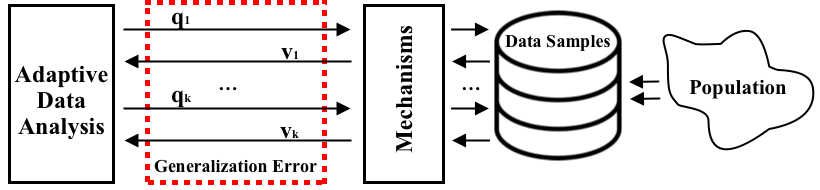
\includegraphics[width=0.9\columnwidth]{chapters/adapt/overview-dissertation.png}
    \caption{Overview of our adaptive data analysis model. }
    \label{fig:adaptivity-model-overview}
\vspace{-0.5cm}
\end{figure}

A line of work initiated by \citet{DworkFHPRR15}, \citet{HardtU14} posed the question: Can we design \emph{general-purpose} methods that ensure generalization in the presence of adaptivity, together with guarantees on their accuracy?  The idea that has emerged in these works is to use randomization to help ensure generalization. Specifically, these works have proposed to mediate the access of an adaptive data analysis to the data by means of queries from some pre-determined family (we will consider here statistical or linear queries) that are sent to a  \emph{mechanism} which uses some randomized process to guarantee that the result of the query does not depend too much on the specific
sampled dataset. This guarantees that the results of the queries generalize well. This approach is described in Figure~\ref{fig:adaptivity-model-overview}.  We have a population that we are interested in studying, and a dataset containing individual samples from this population. The adaptive data analysis we are interested in running has access to the dataset through queries of some pre-determined family (e.g., statistical or linear queries) mediated by a mechanism. This mechanism uses randomization to reduce the generalization error of the queries issued to the data.
This line of work has identified many new algorithmic techniques for ensuring generalization in adaptive data analysis, leading to algorithms with greater statistical power than all previous approaches. Common methods proposed by these works include, the addition of noise to the result of a query, data splitting, etc. Moreover, these works have also identified problematic strategies for adaptive analysis, showing limitations on the statistical power one can hope to achieve. Subsequent works have then further extended the methods and techniques in this approach and further extended the theoretical underpinning of this approach, e.g.~\cite{dwork2015reusable,dwork2015generalization,BassilyNSSSU16,UllmanSNSS18,FeldmanS17,jung2019new,SteinkeZ20,RogersRSSTW20}.
%

A key development in this line of work is that the best method for ensuring generalization in an adaptive data analysis depends to a large extent on the number of \emph{rounds of adaptivity}, the depth of the chain of queries. As an informal example, the program $x \leftarrow q_1(D);y \leftarrow q_2(D,x);z \leftarrow q_3(D,y)$ has three rounds of adaptivity, since $q_2$  depends on $D$ not only directly because it is one of its input but also via the result of $q_1$, which is also run on $D$, and similarly,  $q_3$ depends on $D$ directly but also via the result of $q_2$, which in turn depends on the result of $q_1$. The works we discussed above showed that, not only does the analysis of the generalization error depend on the number of rounds, but knowing the number of rounds actually allows one to choose methods that lead to the smallest possible generalization error. As an example, when a study includes queries with a large number of rounds of adaptivity, then a low generalization error can be achieved by adding Gaussian noise scaled to the number of rounds to the result of each query.
When instead a study includes queries with a low number of rounds of adaptivity, then a low generalization error can be achieved by using more specialized methods, such as the reusable holdout technique from~\citet{DworkFHPRR15}. 


\subsection{Some Results in Adaptive Data Analysis}
In Adaptive Data Analysis an \emph{analyst} is interested in studying some distribution $\dist$ over some domain $\univ$.  Following previous works~\cite{DworkFHPRR15,HardtU14,BassilyNSSSU16}, we focus on the setting where the analyst is interested in answers to \emph{statistical queries} (also known as \emph{linear queries}) over the distribution.  A statistical query is usually defined by some function $\query \from \univ \to [-1,1]$ (often other codomains such as $[0,1]$ or $[-R,+R]$, for some $R$, are considered). \wq{$\mathbb{E}$ represents the expectation.} The analyst wants to learn the \emph{population mean}, which (abusing notation) is defined as $$\query(\dist) = \ex{\sample \sim \dist}{\query(\sample)}.$$

However, the distribution $\dist$ can only be accessed via a set of \emph{samples} $\sample_1,\dots,\sample_n$ drawn from $\dist$. We assume that the samples are drawn independently and identically distributed (i.i.d.).  These samples are held by a mechanism $\mech(\sample_1,\dots,\sample_n)$ who receives the query $\query$ and computes an answer 
$$\answer \approx \query(\dist).$$

The na\"ive way to approximate the population mean is to use the \emph{empirical mean}, which (abusing notation) is defined as $$\query(\sample_1,\dots,\sample_n) = \frac{1}{n} \sum_{i=1}^{n} \query(X_i).$$
However, the mechanism $M$ can then adopt some methods for improving the generalization error.

In this work, we consider analysts that ask a sequence of $\qlen$ queries $\query_1,\dots,\query_\qlen$.  If the queries are all chosen in advance, independently of the answers of each one of them, then we say they are \emph{non-adaptive}.  If the choice of each query $\query_j$ depend on the prefix $\query_1,\answer_1,\dots,\query_{j-1},\answer_{j-1}$ then they are \emph{fully adaptive}.  An important intermediate notion is \emph{$\qrounds$-round adaptive}, where the sequence can be partitioned into $\qrounds$ batches of non-adaptive queries.  Note that non-interactive queries are $1$-round and fully adaptive queries are $\qlen$ rounds.

We now review what is known about the problem of answering $r$-round adaptive queries.  
\begin{thm} 
\label{thm:nonadapt-adapt}
For any distribution $\dist$, and any $k$ \emph{non-adaptive} statistical queries, the empirical mean satisfies
$$
\max_{j=1,\dots,\qlen} | \answer_j - \query_j(\dist) | = O\left( \sqrt{\frac{\log \qlen}{n}}  \right)
$$
For any $\qrounds \geq 2$ and any \emph{$\qrounds$-round adaptive} statistical queries, it satisfies
$$
\max_{j=1,\dots,\qlen} | \answer_j - \query_j(\dist) | = O\left( \sqrt{\frac{\qlen}{n}}  \right)
$$
\end{thm}
These bounds are tight (up to constant factors) which means that even allowing one extra round of adaptivity leads to an exponential increase in the generalization error of the empirical mean, from $\log \qlen$ to $\qlen$.

\citet{DworkFHPRR15} and \citet{BassilyNSSSU16} showed that by using an alternative mechanism $M$ which uses randomization in order to limit the dependency of a single query on the specific data instance, one 
can actually achieve a much stronger generalization error as a function of the number of queries, specifically.
\begin{thm}[\cite{DworkFHPRR15, BassilyNSSSU16}] \label{thm:gaussiannoise} For any $k$, there exists a mechanism such that for any distribution $\dist$, and any $\qrounds \geq 2$ any \emph{$\qrounds$-round adaptive} statistical queries, it satisfies
$$
\max_{j=1,\dots,\qlen} | \answer_j - \query_j(\dist) | = O\left( \frac{\sqrt[4]{\qlen}}{\sqrt{n}}  \right)
$$
%And there is an analyst that make this bound tight (up to constant factors).
\end{thm}
Notice that Theorem~\ref{thm:gaussiannoise} has different quantification in that the optimal choice of the mechanism depends on the number of queries.  Thus, we need to know the number of queries \emph{a priori} to choose the best mechanism.
% \footnote{ \label{fn1} One can, in principle, avoid knowing the number of queries and rounds \emph{a priori} using a ``guess-and-double'' strategy, however this would weaken the bound on generalization error considerably.}


%Later work by Dwork 
% \etal~\cite{??} 
\citet{DworkFHPRR15}
also gave more refined bounds in terms of the number of rounds of adaptivity.   %\footnotemark[\ref{fn1}] 
%Specifically, 
\begin{thm}[\cite{DworkFHPRR15}] \label{thm:gaussiannoise2} For any $r$ and $k$, there exists a mechanism such that for any distribution $\dist$, and any $\qrounds \geq 2$ any \emph{$\qrounds$-round adaptive} statistical queries, it satisfies
$$
\max_{j=1,\dots,\qlen} | \answer_j - \query_j(\dist) | = O\left( \frac{r \sqrt{\log k}}{\sqrt{n}}  \right)
$$
%And there is an analyst that make this bound tight (up to constant factors).
\end{thm}

This suggests that if one knows a good \emph{a priori upper bound on the number of rounds of adaptivity}, one can get a much better guarantee of the generalization error, but only by using an appropriate choice of the mechanism.




%gap
This scenario motivates us to explore the design of program analysis techniques that can be used to estimate the number of \emph{rounds of adaptivity} that a program implementing a data analysis can perform. These techniques could be ultimately be integrated into a tool for adaptive data analysis such as the \emph{Guess and Check} framework by~\citet{RogersRSSTW20}. 
%

\section{Challenges and Our solutions }
\label{sec:adapt-challenges}

\subsection{Formalizing an Adaptive Data Analysis Model}
\label{subsec:adapt-formalizing-model}
The first problem we face is \emph{how to define formally} a model for adaptive data analysis which is general enough to support the methods we discussed above and would permit to formulate the notion of adaptivity these methods use. We take the approach of designing a programming framework for submitting queries to some \emph{mechanism} giving access to the data mediated by one of the techniques we mentioned before, e.g., adding Gaussian noise, randomly selecting a subset of the data, using the reusable holdout technique, etc. In this approach, a program models an \emph{analyst} asking a sequence of queries to the mechanism. The mechanism runs the queries on the data applying one of the methods discussed above and returns the result to the program. The program can then use this result to decide which query to run next. Overall, we are interested in controlling the generalization of the results of the queries which are returned by the mechanism, by means of the adaptivity. 

To define adaptivity we consider a dependency graph between the different queries that we synthesize from the possible execution traces of the program representing the data analysis. The dependency graph is built by inspecting all the possible traces of execution and by identifying situations where the execution of a query \emph{causes} the execution of another query. Intuitively, a query $Q$ may depend on another query $P$, if there are two values that $P$ can return which affect in different ways the execution of $Q$. 
For example, as depicted in \cite{dwork2015reusable}, a machine learning algorithm for constructing a classifier can be modeled by first computing each feature's correlations with the label via a sequence of queries and then constructing the classifier based on the correlation values. If one feature's correlation changes, the classifier depending on features is also affected.  
This notion of dependency builds on the execution trace as a \emph{causal history}. In particular, we are interested in the history or provenance of a query up until this is executed, we are not then concerned about how the result is used --- except for tracking whether the result of the query may further cause some other query. This is because we focus on the generalization error of queries and not their post-processing.  

\paragraph{Through an Example}
 We motivate the definition of adaptivity we will use through a simple example illustrated in Figure~\ref{fig:simpl-two-round-graph}(a), which implements a simple "two rounds strategy".

%
% Figure~\ref{fig:simpl-two-round-graph}.  
{
\begin{figure}
%\begin{equation*}
%\label{}
% \[
%TR(k) \triangleq
%{
\centering
\begin{subfigure}{.2\textwidth}
\begin{centering}
$
\begin{array}{l}
   a \leftarrow 0; \\
   i \leftarrow 0 ; \\
    \eloop ~ 3 ~ \edo ~ \\
    \quad
     x \leftarrow q_1(\chi[i])   ; \\
    \quad a \leftarrow a+x; \\
        \quad i \leftarrow i+1; \\
    l \leftarrow q_2(\chi[4]*a)\\
\end{array}
$
\caption{}
\end{centering}
\end{subfigure}
%}
\quad
\begin{subfigure}{.2\textwidth}
\begin{centering}
$
\begin{array}{l}
   \clabel{ a \leftarrow 0}^{1}; \\
   \clabel{ i \leftarrow 0}^{2} ; \\
    \eloop ~ \clabel{3}^{3} ~ \edo ~ \\
    \quad
    \clabel{ x \leftarrow q_1(\chi[i])}^{4}   ; \\
    \quad \clabel{a \leftarrow a+x}^{5}; \\
        \quad \clabel{i \leftarrow i+1}^{6}; \\
    \clabel{l \leftarrow q_2(\chi[4]*a)}^{7}\\
\end{array}
$
\caption{}
\end{centering}
\end{subfigure}
\begin{subfigure}{.55\textwidth}
%}
\qquad
\begin{centering}
$\vcenter{\hbox{
% \]
% \begin{wrapfigure}{R}{0.5\textwidth}
% \begin{figure}
% \begin{tcolorbox}[colback=white]
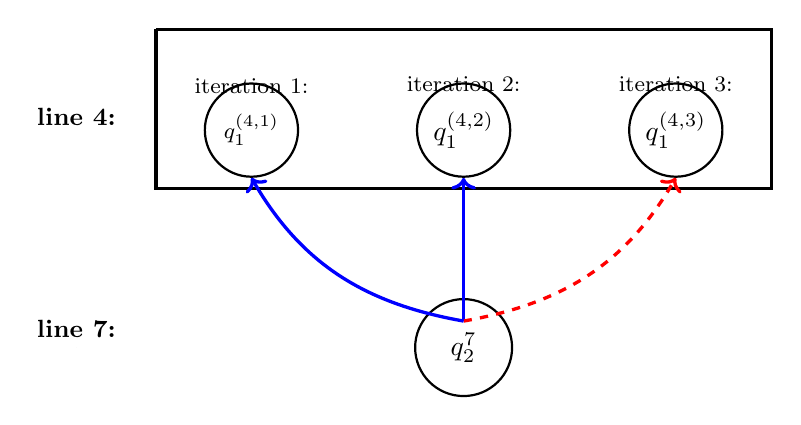
\begin{tikzpicture}[scale=\textwidth/18cm,samples=200]
%%% The nodes represents the k query in the first round
\draw[very thick] (0.2,6)  -- (11.8,6) -- (11.8,3) -- (0.2,3) -- (0.2,6);
\draw[black] (-1.3, 4) circle (0pt) node [anchor=south]{\small{\textbf{line 4:}}};
\filldraw[black] (-1.3, 0) circle (0pt) node [anchor=south]{\small{\textbf{line 7:}}};
%
\draw[thick] (2, 4.1) circle (25pt) 
node[label={above: \footnotesize{iteration 1:}}] {\footnotesize{$q_1^{(4,1)}$}} ;
\draw[thick] (6, 4.1) circle (25pt) node[label={[black]above: \footnotesize{iteration 2:}}] 
{$q_1^{(4,2)}$};
\draw[thick] (10, 4.1) circle (25pt) node [label={[black]above: \footnotesize{iteration 3:}}]
{$q_1^{(4,3)}$};
\draw[thick] (6, 0) circle (26pt) node {$q_2^7$};
\draw[very thick,->, blue] (6, 0.5)  -- (6, 3.2) ;
\draw[very thick,->, red, dashed] (6, 0.5)  to [out=10,in=240] (10, 3.2) ;
\draw[very thick,->, blue] (6, 0.5)  to [out=170,in=300]  (2, 3.2) ;
\end{tikzpicture}
}
}
$
\caption{}
\end{centering}
\end{subfigure}
% \end{wrapfigure}
% \end{equation*}
\vspace{-0.4cm}
 \caption{(a) Example of a program with two rounds of adaptivity, (b) Labeled program for the same example, (c) The corresponding query-based dependency graph.}
\label{fig:simpl-two-round-graph}
\vspace{-0.5cm}
\end{figure}
}
 %
 %
% \mg{I don't think the example is good enough. Specifically, I think that we should use the rows of the database somewhere, we don't use them at all in the example. Also, do we have bounds that depend on a variable? I thought we had only loops with constants. I sketched something that could work for us.}

In this example, the analyst asks queries to the mechanism in two phases. In the first phase,  the analyst asks a fixed number $k$ of queries (in the example $k=3$) and stores the answers that are provided by the mechanism. In the second phase, the analyst constructs a new query based on the results of the previous $k$ queries and sends this query to the mechanism. More specifically, we assume that, in this example, the domain $X$ contains at least four numeric attributes, which we index just by natural numbers. The queries inside the loop correspond to the first phase and compute an approximation of the empirical mean of the first three attributes. The query outside the loop corresponds to the second phase and computes an approximation of the empirical mean where each record is weighted by the sum of the empirical mean of the first three attributes. 
%
Queries are of the form $q(e_q)$ where $e_q$ is a query expression with a special variable $\chi$ representing a possible row. Mainly $e_q$ represents a function from $X$ to some domain $U$, for example $U$ could be $[-1,1]$ or $[0,1]$. This function characterizes the linear query we are interested in running. As an example, $x \leftarrow q(\chi[2])$ computes an approximation, according to the used mechanism, of the empirical mean of the second attribute, identified by $\chi[2]$. Notice that we don't materialize the mechanism but we assume that it is implicitly run when we execute the query.  

% a predicate  (the sum in this example). The program in the {\tt Loop} language implementing this algorithm is presented in Figure~\ref{fig:simpl-two-round-graph}(a). The answers in the first round are accumulated in variable $a$. The index $i$ is a loop counter used to express $k$(we pick $k=3$) queries $q_1(\chi[i])$ of the first round. The query $q_2(\chi[4]+a)$ in the second round uses $a$.} 

 In order to analyze programs like the one we just discussed, it is convenient to work with a version of the program where similar commands can be easily distinguished. For this reason, we use labeled versions of programs, where labels correspond to lines of code. As an example, we give the labeled version of the two rounds example program in Figure~\ref{fig:simpl-two-round-graph}(b).
%  We leave
%  more details about the labeled {\tt Loop} language in Section~\ref{sec:loop_language}. 
%  When we try to analyze this program, we run quickly into the issue that queries of the form $q(e)$ can be run multiple times with different values for $e$ since variables can be reassigned. To identify variables For instance, look at aforementioned program of two round strategy, variable $a$ used at line $7$ comes from the assignment at line $5$ instead of line $1$. To avoid this confusion, we add line numbers(we call it label) to commands. The labelled one is shown in Figure~\ref{fig:simpl-two-round-graph}(b).
%  We leave
%  more details about the labelled {\tt Loop} language in Section~\ref{sec:loop_language}. 

% Our framework aims to provides an upper bound on the number of rounds of adaptivity (or the depth of chain of queries connected by dependency relation), denoted as $A$ in the Fig~\ref{fig:structure}, of a high level program $P$. We will go through one concrete example called "two rounds algorithm"  after the brief introduction of high level loop language, in which the target program ($TR^{H}$) implementing "two rounds algorithm" is written.

% In the high level loop language, the assignment command $x \leftarrow e$ and the loop command $\eloop ~ \aexpr  ~ \edo ~ c $ is standard. The command $ \assign{x} {q(\expr)}$ stores the result of a query $q(\expr)$ in which the elements used to construct the query are presented by the expression $\expr$. 
% We have the standard arithmatic operators denoted as $\opuls_a$, boolean operators as $\oplus_b$, and relational operators as $*_r$. 
% \[
% \begin{array}{llll}
% %  \mbox{Arithmatic Operators} & *_a & ::= & + ~|~ - ~|~ \times 
% % %
% % ~|~ \div \\  
% %   \mbox{Boolean Operators} & *_b & ::= & \lor ~|~ \land ~|~ \neg\\
% %   %
% %   \mbox{Relational Operators} & *_r & ::= & < ~|~ \leq ~|~ = \\  
% \mbox{AExpr} & \aexpr & ::= & 
% 	n ~|~ x ~|~ \aexpr *_a \aexpr ~|~ {[] ~|~ [\aexpr_0, \dots, \aexpr_i]  }  \\
% \mbox{BExpr} & \bexpr & ::= & 
% 	\etrue ~|~ \efalse  ~|~ \neg \bexpr
% 	 ~|~ \bexpr *_b \bexpr
% 	~|~ \aexpr *_r \aexpr \\
% \mbox{Command} & c & ::= &   \assign{x}{\expr} ~|~  \assign{x} {q(\expr)} ~|~  c ; c ~|~ \eif(\bexpr, c_1, c_2) 
% 	 ~|~ \eskip \sep {\eloop ~ \aexpr  ~ \edo ~ c }
% \end{array}
% \]

This example is intuitively 2-rounds adaptive. The reason is that we have two distinguished phases and the queries that we ask in the first phase do not depend on each other, while the last query depends on all the previous queries. 
However, capturing this concept formally is surprisingly difficult. The difficulty comes from the fact that a query can depend on the result of another query in multiple ways, by means of data dependency or control flow dependency. In order to find the right definition for our goal, we take inspiration from the known results of the data analysis model we discussed above. This theory tells us that what we want to measure is the generalization error on the result of a query and not an arbitrary manipulation of the query. Indeed, arbitrary manipulations can change the generalization error. As an example, suppose that $v$ is the result we get from running a query, if we multiply this result by some constant, we are also changing the incurred error. Moreover, this theory tells us that we can always consider a non-adaptive set of queries as to being adaptive, and more importantly, that we can transform an adaptive query into a non-adaptive one, incurring an exponential blow-up of the number of queries. For example, we could ask many queries upfront, and depending on the results of some of them, we could return the results of others. For these reasons, we define adaptivity in terms of the possible execution traces of the program on all possible inputs. A trace of execution is a list of query requests of the form $[q(v_1)^{(l_1,w_1)},\ldots, q(v_n)^{(l_n,w_n)}]$, where every occurrence of a query is labeled with the line of code $l$ it appears at, and the counter $w$ identifying the possible loop iteration happening when a query is called. For example, in $q(v_1)^{(3,1)}$, the superscript $(3,1)$ indicates that the query is asked at line $3$ and that the query is requested in the first iteration of the loop. When the query is not in a loop, we omit the counter.

Using traces we can identify situations when one query can affect the execution of another one. Using this information we can build a directed graph, called the query-based dependency graph, where the nodes represent the queries that are executed and the edges between two nodes represent the fact that one query may depend on the other. We show such a graph for our running example in Figure~\ref{fig:simpl-two-round-graph}(c). We can then define adaptivity as the longest possible path in this graph.  Looking again at our example, it is easy to see that the longest path in the graph in Figure~\ref{fig:simpl-two-round-graph}(c), which we mark with a red dashed arrow, is $2$, as we were expecting.

% \wq{
%  Now that we we look at the adaptivity of this example. First of all, to apply the theorems described above, the adaptivity is achieved in the setting that the analyst is only interested in the answers to the sequence of linear queries he/she asks to the mechanism. So the adaptivity of this two round strategy can be obtained by finding out a sequence of adaptively chosen queries with longest length, among all the queries the analyst asks. Intuitively, this longest sequence of adaptively chosen queries can be transformed to, the longest path in a directed graph where the node representing the queries asked and the edge between two nodes standing for one query may depend on the other. We show such a graph in Figure~\ref{fig:simpl-two-round-graph}(c), and call it, query-based dependency graph. In the graph, every node stands for a query with annotation. 
% }
% \wq{To draw the query-based dependency graph, we need to consider two components: the vertices and the edges. Our approach is defined as follows. 
% \begin{enumerate}
%     \item The vertices are collected by a trace-based operational semantics, which tracks the execution of the program.
%     \item The edges are defined by a formal definition of may-dependency between two queries.
% \end{enumerate}
% }
  % trace operation semantics
%   The trace-based operational semantics of the loop language have the shape of $\config{m, c, t,w} \xrightarrow{} \config{m', c',  t', w'}  $. It works on a configuration of memory $m$, a program $c$, a trace $t$, a loop map $w$. The trace $t$ is a list of annotated queries. One annotated query is a  
%   query with the annotation $(l,w)$, $l$ is the line number and $w$ is used for loop and tells the iteration number. For example, the 
%   query $q()$ at line $3$ in the example $TR$ at the first iteration is represented as the annotated query $q()^{(3, [2:1])}$. The loop map $w$ is a map, from the line number of the loop counter ( $\clabel{k}^{2}$ ) to its iteration number. The trace tracks the query asked during the execution, still use the $TR$ as an example. The trace of $TR$ starting with an empty loop map $\emptyset$ has the following trace $t_{tr}$, supposing $k=3$. 
%   \[t_{tr} = [q()^{(3,[2:1])},q()^{(3,[2:2])},q()^{(3,[2:3])}, q(a)^{(5,\emptyset)}  ] \]
  
% % define rounds of adaptivity
% The second component is the defintion of may-dependency between queries. In particular, what we need to be clear is what does it mean by saying one query may depend on another query. To this end, we look at trace.  Now whether one query $q$ depends on another query $p$ can be checked, by witnessing $q$ in the new generated trace upon change of $p$. For example, if we change the result of $q()^{(3,[2:1])}$, we have a new trace $t'_{tr}$, and $a$ may change as well. In this case, $q(a)^{(5, \emptyset)}$ may not show up in the new generated trace $t'_{tr}$. So we think $q(a)^{(5, \emptyset)}$ may depend on $q()^{(3,[2:1])}$. 
% trace based dependency relation is challenging

\begin{figure}
    \centering    
    \begin{tikzpicture}
    % {node distance = 2cm, auto}
  % nodes
%   \node[block] at (2,-6) (block6) {$f_6$};
  \node [block][text width=8em](high){ Program $P$ } ;
  \node [block, right of = high, node distance = 7cm, text width=13em](ssa){SSA Program $P^{s}$} ;
  \node [block, below of = ssa, node distance = 2cm, text width=13em] (bound) {Estimated Adaptivity $Adapt$} ;
  \node [block, below of = high, node distance = 2cm, text width=8em](adapthigh){Adaptivity $A$};
  % edges
  \path [line, thick] (high) -- node [above] {transformation} (ssa) ;
  \path [line, thick] (ssa) -- node [label={[label distance=.2cm]0:\ADAPTSYSTEM}] {} (bound);
  \path [line, thick] (bound) -- node [below] {upper bound} (adapthigh);
  \path [line, thick]  (high) -- node [label={[label distance=-3cm]0:trace-based graph}]{}(adapthigh);   
 \end{tikzpicture} 
   \caption{High level architecture of {\ADAPTSYSTEM}.}
    \label{fig:structure}
\end{figure}


\subsection{Static Analysis for Adaptivity}

The second problem we face is \emph{how to estimate the adaptivity of a given program}. The adaptive data analysis model we consider and our definition of adaptivity suggest that for this task we can use a  program analysis that is reminiscent of information flow control. However, this is not sufficient since, in general, a query $Q$ is not a monolithic block but rather it may depend, through the use of variables and values, on other parts of the program. Hence, we also need to consider some form of data-flow analysis. Our program analysis, named {\ADAPTSYSTEM}, combines information flow and data-flow analysis using an adjacency matrix $M$ representing the dependency between different variables, and a vector $V$ representing different queries. These two components allow us to over-approximate the dependency graph and estimate the adaptivity of the program. 

To simplify our analysis, we do not directly apply the program analysis to the source program. Instead, we first transform the program into static single assignment form, SSA form. In this form all the variables are assigned once, including variables in loops, and this helps our analysis in avoiding the complexity of handling variables reassignment. Moreover, we show that by analyzing programs in SSA form, we get a bound on the number of rounds of adaptivity that is also a bound for the source program.

The high-level architecture of our static analysis framework is shown in 
 Figure~\ref{fig:structure}. The input of the analysis is a labeled program P for which the adaptivity A is defined by means of a trace-based definition, as discussed above. In order to estimate an upper bound on A, our program analysis first transforms the program P into the static single assignment (SSA) form. The goal of this step is to guarantee that each variable is assigned only once. We show the result of this transformation applied to our two rounds strategy example in Figure~\ref{fig:ssa_tworound}(a). 
 This transformation, when applied to a loop, introduces some extra variables that serve as intermediate storage. For example, in~\ref{fig:ssa_tworound}(a) there is a new instruction $[(i_3,i_1,i_2),(a_3,a_1,a_2)]$ after the loop. This instruction asserts that the value of the new variables $i_3$ and $a_3$, depending on the execution step, may come from $i_1$ or $i_2$, $a_1$ or $a_2$, respectively. \wq{To be concrete, if it is in the first iteration of the loop, $i_3 = i_1$, otherwise, $i_3 = i_2$.} For those readers who are familiar with SSA, it can be regarded as another form of the phi node. The transformation of a program into SSA form preserves the execution traces, and so, in turns, it preserves the adaptivity. 

\begin{figure} 
\centering
   \begin{subfigure}{.2\textwidth}
   \begin{centering}
   $
   \begin{array}{l}
  \clabel{ a_1 \leftarrow 0}^{1}; \\
   \clabel{ i_1 \leftarrow 0}^{2} ; \\
    \eloop ~ \clabel{3}^{3} ~ \edo ~ \\ 
    \quad [(i_3, i_1,i_2), (a_3,a_2,a_1)] \\
    %  \quad i_3 = \phi(i_1,i_2); \\
    %   \quad a_3 = \phi(a_1,a_2); \\
    \quad
    \clabel{ x_1 \leftarrow q_1(\chi[i_3])}^{4}   ; \\
    \quad \clabel{a_2 \leftarrow a_3+x_1}^{5}; \\
        \quad \clabel{i_2 \leftarrow i_3+1}^{6}; \\
    \clabel{l_1 \leftarrow q_2(\chi[4]*a_3)}^{7}\\
    \end{array}
% {
% \begin{array}{l}
%   \clabel{ a_1 \leftarrow [] }^{1}; \\
%     \eloop ~ \clabel{k}^{2} ~ \edo ~ \\
%     \Big(
%       a_3 = \phi(a_1,a_2); \\
%      \clabel{x_1 \leftarrow q() }^{3}  ; \\
%     \clabel{a_2 \leftarrow x :: a_3}^{4}      \Big); \\
%     \clabel{l_1 \leftarrow q(a_3)}^{5}\\
% \end{array}
% }
 $
 \caption{}
   \end{centering}
   \end{subfigure}
   \begin{subfigure}{.5\textwidth}
   \begin{centering}
   $\vcenter{\hbox{
% \]
% \begin{wrapfigure}{R}{0.5\textwidth}
% \begin{figure}
% \begin{tcolorbox}[colback=white]
   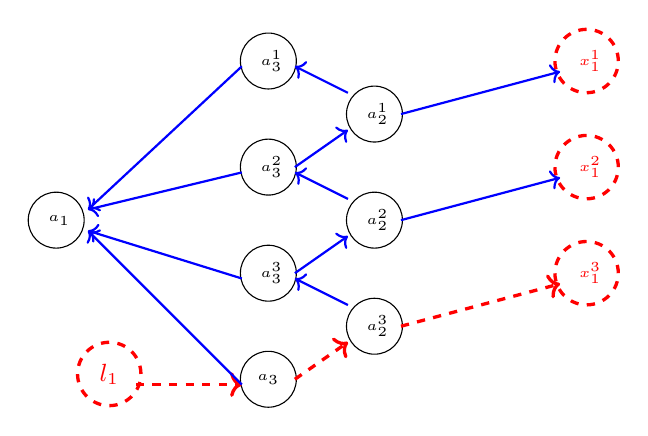
\begin{tikzpicture}[scale=\textwidth/18cm,samples=200]
%%% The nodes represents the k query in the first round
% \draw[very thick] (-1,6)  -- (13,6) -- (13,3) -- (-1,3) -- (-1,6);
% \draw[black] (-2.5, 4) circle (0pt) node [anchor=south]{\textbf{line 4:}};
% \draw[thick] (1, 1.1) circle (25pt) node
% % node[label={above: \small{iteration 1:}}] 
% {\tiny{$q_1^{(5,1)}$}} ;
\draw[] (2, 5.1) circle (15pt) node
{\tiny{ $a_1$}};
\draw[] (6, 8.1) circle (15pt) node
{\tiny{ $a_3^{1}$}};
% \draw[thick] (8, 11.1) circle (15pt) node
% {\tiny{ $x_{1}^{1}$}};
% \draw[thick] (10, 10.1) circle (15pt) node
% {\tiny{ $x_{2}^{1}$}};
\draw[very thick, dashed, red] (12, 8.1) circle (17pt) node{\tiny{\textbf{ $x_{1}^{1}$}}};
\draw[] (8, 7.1) circle (15pt) node
{\tiny{ $a_{2}^{1}$}};
\draw[] (6, 6.1) circle (15pt) node{\tiny{ $a_3^{2}$}};
% \draw[thick] (10, 8.1) circle (15pt) node
% {\tiny{ $x_{1}^{2}$}};
% \draw[thick] (12, 7.1) circle (15pt) node
% {\tiny{ $x_{2}^{2}$}};
\draw[very thick, dashed, red] (12, 6.1) circle (17pt) node{\tiny{\textbf{ $x_{1}^{2}$}}};
\draw[] (8, 5.1) circle (15pt) node
{\tiny{ $a_{2}^{2}$}};
% \draw[thick] (12, 5.1) circle (15pt) node
% {\tiny{ $x_1^{3}$}};
\draw[] (6, 4.1) circle (15pt) node
{\tiny{ $a_3^{3}$}};
\draw[very thick, dashed, red] (12, 4.1) circle (17pt) node{\tiny{\textbf{ $x_1^{3}$}}};
% \draw[thick] (12, 3.1) circle (15pt) node
% {\tiny{ $x_2^{3}$}};
\draw[] (8, 3.1) circle (15pt) node
{\tiny{ $a_{2}^{3}$}};
 \draw[] (6, 2.1) circle (15pt) node 
{\tiny{$a_3$}};
% \filldraw[black] (-2.5, 0) circle (0pt) node [anchor=south]{\textbf{line 7:}};
\draw[very thick, dashed, red] (3, 2.2) circle (17pt) node {\small{\textbf{$l_1$}}};
%dotted
 \draw[->, red, very thick, dashed] 
         (3.5, 2)  -- (5.5, 2) ;
%   \draw[->, red, very thick,snake=snake, segment amplitude=.4mm,
%          segment length=2mm, line after snake=1mm] 
%          (6, 0.5)  -- (6, 1.6) ;
\draw[->, red, very thick, dashed](6.5, 2.1)  -- (7.5, 2.8) ;
 \draw[->, red, very thick, dashed] (8.5, 3.1)  -- (11.5, 3.9) ;
    \draw[thick,->, blue] (8.5, 5.1)  -- (11.5, 5.9) ;
\draw[thick,->, blue] (8.5, 7.1)  -- (11.5, 7.9) ;
%  \draw[thick,->, blue] (10.5, 4.1)  -- (11.5, 4.8) ;
%   \draw[thick,->, red] (10.5, 4.1)  -- (11.5, 3.3) ;
   \draw[thick,->, blue] (7.5, 3.5)  -- (6.5, 4.0) ;
   \draw[thick,->, blue] (6.5, 4.1)  -- (7.5, 4.8) ;
    %  \draw[thick,->, blue] (10.5, 6.1)  -- (11.5, 6.8) ;
% \draw[thick,->, blue] (10, 6.6)  -- (10, 7.6) ;
\draw[thick,->, blue] (7.5, 5.5)  -- (6.5, 6.0) ;
 \draw[thick,->, blue] (6.5, 6.1)  -- (7.5, 6.8) ;
% \draw[thick,->, blue] (8.5, 9.1)  -- (9.5 , 9.8) ;
% \draw[thick,->, blue] (8, 9.6)  -- (8, 10.6) ;
\draw[thick,->, blue] (7.5, 7.5)  -- (6.5, 8.0) ;
\draw[thick,->, blue] (5.5, 8.0)  -- (2.6, 5.3) ;
\draw[thick,->, blue] (5.5, 6.0)  -- (2.6, 5.3) ;
\draw[thick,->, blue] (5.5, 4.0)  -- (2.6, 4.9) ;
\draw[thick,->, blue] (5.5, 2.0)  -- (2.6, 4.9) ;
% \draw[very thick,->, red] (6, 0.5)  to [out=30,in=240] (11, 3.2) ;
% \draw[very thick,->, blue] (6, 0.5)  to [out=150,in=300]  (1, 3.2) ;
\end{tikzpicture}
}
}
$
\caption{}
   \end{centering}
   \end{subfigure}
    \vspace{-0.3cm}
    \caption{(a) Example of a SSA program with two rounds of adaptivity (b) The corresponding variable-based dependency graph.}
    \vspace{-0.5cm}
    \label{fig:ssa_tworound}
\end{figure}
%

The main component of our framework is an algorithm, which we call ${\ADAPTSYSTEM}$. This algorithm constructs a variable-based weighted directed dependency graph where nodes are annotated variables and edges represent potential dependencies between the variables. We show the variable-based dependency graph for our running two rounds example in Figure~\ref{fig:ssa_tworound}(b). The algorithm builds this dependency graph by traversing the SSA program P$^S$ and collecting the information about dependencies between the different variables in an adjacency matrix $M$, and information about the relations between queries and variables in a vector $V$. The matrix $M$ collects information about both data dependency and control flow dependency. The vector $V$ is used to assign a weight to the different nodes. In particular, to each variable related to a query, the algorithm assigns weight $1$ and to any other variables, the algorithm assigns no weight. The estimated upper bound for the adaptivity is the weight of the path in the graph with maximal weight.  \wq{In Figure~\ref{fig:ssa_tworound}(b), we have a dependency graph between variables. The nodes are the assigned variables and the edge between two nodes means one variable may have data dependency or control flow dependency(or both) on the other variable. Only the variable $x$ which is assigned with the query result via $\assign{x}{q(e_q)}$ will be marked as the weighted node with the unit weight. The nodes in a dashed circle are those special nodes associated with query requests. We want to find the path in the graph with the highest weights (the most special nodes). } The path with maximal weight is the dashed one in the graph. The weight of this path is $2$, providing us a tight upper bound on the adaptivity of P. More in general, we prove that the upper bound estimated by {\ADAPTSYSTEM} gives a sound overapproximation of the adaptivity of the analyzed program. 

% \wq{According to the aforementioned work for ensuring generalization in adaptive data analysis, the tight generalization error bound is achieved under the analyst-mechanism assumption that, the analyzed program is modelled as a procedure of an \emph{analyst} asking a sequence of queries to some mechanism and only the responded answers are back to the {analyst}, with no processing of the query results revealed. Then The adaptivtity notion under this assumption, only focusing on the queries, is the length of a sequence of adaptively chosen queries among the queries asked by the {analyst}.}
% This requires us to define  Since most of these techniques we focus in this work on queries that can be executed \emph{row-by-row}, those submitted 
% queries are specified by some function of a row in the framework.
% and how to integrate the techniques mentioned before in a programming . Hence, as a first step we Nevertheless, the corresponding study on static analysis over programs implementing adaptive analysis is not well explored, even the formal definition of this \emph{rounds of adaptivity} is not clear. Our goal is to study adaptivity and conduct analysis over programs to find the number of rounds.
% our innovation

% Based on this framework, we define adaptivity as a property based on multiple traces of executions, or in other terms as an hyperproperty~\cite{clarkson2010hyperproperties}. \wq{For the sequence of adaptively chosen queries described before, the concept of one query may depend on its previous queries and answers is necessary. } Intuitively, a query $Q$ may depend on another query $P$, if there are two 
% values that $P$ can return which affect in different ways the execution of $Q$. 
% This definition suggests that we need to consider a program analysis which is a reminiscence of information flow control. However, this is not sufficient since, in general, a query is not a monolithic block $Q$ but rather some syntactic construction depending on some expression that depends on some variables. Hence, we also need to consider some data-flow analysis. 
% In a word, what we want is a program analysis which statically provides an upper bound on the number of rounds of adaptivity, and on the number of queries that are run by programs implementing adaptive data analysis. 

% The first question we need to decide on is what language the target programs to be analyzed are written, in a functional programming language or an imperative one?     
% the reason we do not use functional programming language, 
 %We choose the imperative programming language, then the following question is what does this imperative language look like? 
%  A principle of the ideal language in our mind is supposed to be simple enough to alleviate the burden of analysis on complex components that is unnecessary to adpativity, and expressive enough to support most of the adaptive data analysis algorithms. With this principle in mind, we introduce an imperative language called the {\tt Loop} language, with one finite loop construct, allowing data analysts recursively request queries in their programs. The query request is also supported in the language.

% The query request is abstract in the loop language and shows up as a primitive construct $q(e)$, where the argument $e$ is an expression tracking the necessary information needed to construct the unique query. We choose to make query abstract for the reason that we only care about the elements(the arguments) used to construct the query instead the detail of the query, with respect to what we are interested in: whether some queries rely on some other queries.        

%  For the number of rounds of adaptivity of program in the loop language, a definition of "one query relies on another query", or "one query may depend on the other" is the next big thing. We choose to define this "may-dependency" with the help of a trace-based operational semantics.  
% %  the change of the results of the query will affect the appearance of the other in a trace of the execution. The trace is
%  The trace is a list of queries generated along with the execution of the program, a history of the execution only caring about query requests.
%  which is specified in the operational semantics and will be discussed later.


% one is the transformation of programs of the aforementioned loop language we call it "high level language", to its variant "low level language", in which the arguments of queries go into the control flow of the program. Performing such a transformation helps us to better focus on the dependency between queries because we can treat queries simply as primitive symbols in the low level loop language without worrying about the arguments of the queries affecting the results. 
% In a word, the key idea of this transformation guarantees all the effect on queries comes from the structure of the programs. 
% The other is the transformation from the "low level" programs
% to construct a dependency graph between these unique variables, and hence predict the rounds of adaptivity from the graph. To generate the dependency graph, 
% To be more specific, our framework is equipped with algorithms to record the necessary information and construct a dependency graph to reach a final estimation of the adaptivity.
\section{Contributions of {\ADAPTSYSTEM}}
\label{sec:adapt-contributions}
To Summarize, our work aims at the design of a static analysis for programs implementing adaptive analysis that can estimate their rounds of adaptivity. Specifically, our contributions are as follows:
\begin{enumerate}
    \item A programming framework for adaptive data analyses where the program represents an analyst that can query a generalization-preserving mechanism mediating the access to some data. 
    % \item A trace-based operational semantics for the loop language, specific to dependency between queries.
    \item A formal definition of the notion of adaptivity under the aforementioned analyst-mechanism model. This definition is built on a query-based dependency graph built out of all the possible program execution traces.
    % \item A transformation between the {\tt Loop} language and the ssa language, with the soundness of the transformation.
    \item A program analysis algorithm {\ADAPTSYSTEM} which provides an estimated upper bound on the adaptivity via a variable-based dependency graph.
    \item A soundness proof of the program analysis showing that the adaptivity estimated by {\ADAPTSYSTEM} bounds the true adaptivity of the program. 
\end{enumerate}




\cleardoublepage

\chapter{Formal Definition of Adaptivity}
\label{ch:adapt-definition}
In this chapter, we formally introduce the language we will focus on for writing data analyses.  
This is a simple loop language with some primitives for calling queries. 
After defining the syntax of the language and showing an example, we will define its trace-based operational semantics. This is the main technical ingredient we will use to define the program's adaptivity.
% We will conclude this chapter by discussing the limitation of this language with respect to static analysis for adaptivity.

\section{Syntax of Query While Language}
\label{sec:adapt-syntax}

\section{ Trace-based Operational Semantics}
\label{sec:adapt-os}
%

\section{ Execution-Based Dependency Graph}
\label{sec:adapt_dynamic}
%

\clearpage

\chapter{The SSA Loop Language}
\label{ch:adapt-ssa}

 This chapter contains the SSA version of the loop language we use to express the data analysis algorithm. Also, the necessity of the transformation from the loop language to the SSA language is presented.

\section{The Limitations of {Loop} Language for Static Analysis}
\label{sec:adapt-limit}
 The labeled {loop} language supports the notion of adaptivity semantically, through a query-based dependency graph. However, syntactically, it is not so suitable for program analysis. The reason is that it allows variables to be reassigned, making the decision on where used variables come from tricky, especially there are controlled branches. We use three examples in {loop} language to show the dilemma, assuming $q_1,q_2,q_3$ are three linear queries.
%
\[
 s_1 = \begin{array}{l}
      \clabel{ \assign{x}{q_1}}^{1} ; \\
      \eif  [(x < 0 )]^{2} \\
      \ethen \clabel{\assign{x}{q_2}}^{3}\\
      \eelse \clabel{\eskip}^{4} ; \\
      \clabel{\assign{y}{q(x+\chi[3])}}^{5}
 \end{array}
 ~~~~~
  s_2 = \begin{array}{l}
      \clabel{ \assign{x}{q_1}}^{1} ; \\
      \eif  [(x < 0 )]^{2} \\
      \ethen \clabel{\assign{x}{q_2}}^{3}\\
      \eelse \clabel{\assign{x}{q_3}}^{4} ; \\
      \clabel{\assign{y}{q(x+\chi[3])}}^{5}
 \end{array}
 ~~~~~~~~
  s_3 = \begin{array}{l}
      \clabel{ \assign{x}{q_1}}^{1} ; \\
      \eif  [(x < 0 )]^{2} \\
      \ethen \clabel{\assign{z}{q_2}}^{3}\\
      \eelse \clabel{\eskip}^{4} ; \\
      \clabel{\assign{y}{q(x+\chi[3]}}^{5}
 \end{array}
\]
In these three examples, the variable $x$ used in the query $q(x+\chi[3])$ at line $5$ is implicit, when we statically analyze the statement $\clabel{\assign{y}{q(x+\chi[3])}}^{5}$. In program $s_1$, it refers to the either $x$ at line $1$, or $x$ at line $3$.  When we have a look at the other two programs $s_2$ and $s_3$, the query $q(x+\chi[3])$ may depend on either $q_2$($x$ at line $3$) or $q_3$($x$ at line $4$) in $s_2$, while it only depends on $q_1$ at line $1$ in program $s_3$. These structural similar three examples, however, have quite dissimilar dependencies between variables. It increases the challenge to track dependency in static analysis. Still look at the analysis on the statement $\clabel{\assign{y}{q(x+\chi[3])}}^{5}$, extra information is needed such as value of $x$ used in the statement may come from the result of $q_1$ or the answer to $q_2$ when this statement lies in $s_1$. Similarly, when in program $s_2$, the extra information that the value of $x$ used in the same statement relies on answers to queries $q_2$ or $q_3$ in both branches of the if statement starting from line $2$ is necessary for static analysis on dependency. Additionally, in program $s_2$, we also need to update the information that $x$ assigned at line $1$ is overwritten by both branches when analyzing the statement at line $5$.   

To simplify the program analysis, we choose to conduct the static analysis on the SSA form of our target programs.   
%
%
%
%  \dg{I am failing to see the problem here. Definition 1 seems to work perfectly well on the above programs and it gives the intuitively correct dependencies. Why do we need SSA?}\wq{The reason to use ssa is to simplify the static analysis in section 5. in $s_2$, when we analyze the command $\assign{y}{q(x+\chi(3))}$, we want to track the information $y$ may depend on $x$, but on which $x$,  at line $3$ or $4$, or even at line $1$? ssa gives us a explicit variable $x_4$ here. }
\[
 s_1^{s} = \begin{array}{l}
      \clabel{ \assign{{\ssa{x_1}}}{q_1}}^{1} ; \\
      \eif  [({\ssa{x_1} }< 0 )]^{2}\\
      ([], [{ \ssa{x_3, x_1,x_2} }], []) \\
      \ethen \clabel{\assign{{\ssa{x_2}}}{q_2}}^{3}\\
      \eelse \clabel{\eskip}^{4} ; \\
      \clabel{\assign{{\ssa{y_1}}}{q({\ssa{x_3} + \chi[3]})}}^{5}
 \end{array}
 ~~~~~
  s_2^{s} = \begin{array}{l}
      \clabel{ \assign{{\ssa{x_1}}}{q_1}}^{1} ; \\
      \eif  [({\ssa{x_1}} < 0 )]^{2} \\
      ( [{\ssa{x_4, x_2,x_3}}], [], [] ) \\
      \ethen \clabel{\assign{{\ssa{x_2}}}{q_2}}^{3}\\
      \eelse \clabel{\assign{{\ssa{x_3}}}{q_3}}^{4} ; \\
      \clabel{\assign{{\ssa{y_1}}}{q({\ssa{x_4}}+\chi[3])}}^{5}
 \end{array}
 ~~~~~~~~
  s_3^{s} = \begin{array}{l}
      \clabel{ \assign{{\ssa{x_1}}}{q_1}}^{1} ; \\
      \eif  [({\ssa{x_1}} < 0 )]^{2} \\
       ( [], [], [] ) \\
      \ethen \clabel{\assign{{\ssa{z_1}}}{q_2}}^{3}\\
      \eelse \clabel{\eskip}^{4} ; \\
      \clabel{\assign{{\ssa{y_1}}}{q({\ssa{x_1}}+\chi[3])}}^{5}
 \end{array}
\]
%
To distinguish between the {loop} language and in SSA form, we denote the SSA variable ${\ssa{x}}$ in bold. As we can see, the reachability of assigned variables becomes explicit in the SSA form. In the SSA version $s_1^s$ of $s_1$, still looking at the statement at line $5$, which becomes $\clabel{\assign{{\ssa{y_1}}}{q({\ssa{x_1}}+\chi[3])}}^{5} $, we can syntactically figure out that the query may depend on the variable $\ssa{x_3}$, which may come from $\ssa{x_1}$ or $\ssa{x_2}$, without extra information like in $s_1$. This benefit also applies to the analysis over the same statement at line $5$ in $s_2^s$ and $s_3^s$.  



\section{Syntax of the SSA Loop Language }
\label{sec:adapt-syntax-ssa-loop}
We present the syntax of the SSA loop language, a language based on the {loop} language, representing programs in the static single assignment form.
% We omit the standard parts inherited from the {loop} language and only present the syntax relevant to ssa. 
% \dg{In the earlier (non-SSA) language, lists were at the level of expressions; now they are at the level of arithmetic expressions. Is this intentional?}\wq{We just decide to change the syntax in the {loop} language, the ssa langauge will be the same, will modify it.}

The expressions inherit from the {loop} language, except that the SSA arithmetic expressions $\ssa{\aexpr}$ now contain SSA variable $\ssa{x} \in \mathcal{SV}$. The boolean expressions in the SSA loop language are denoted as $\ssa{\bexpr}$. In the language, variables can also be annotated, denoted as $\mathcal{LV}$, in a similar way as the annotated queries in the {loop} language. For instance, $\ssa{x}^{(l,w)} \in  \mathcal{LV}$. The SSA memory now is a map from SSA variables to values.
%

The SSA labeled command $\ssa{c}$ inherits from the {loop} language, except that the expressions and variables in these commands are now in its SSA version as shown below. 
\[
\begin{array}{llll}
%  \mbox{Arithmatic Operators} & \oplus_a & ::= & + ~|~ - ~|~ \times 
% %
% ~|~ \div \\  
%   \mbox{Boolean Operators} & \oplus_b & ::= & \lor ~|~ \land ~|~ \neg\\
%   %
%   \mbox{Relational Operators} & \sim & ::= & < ~|~ \leq ~|~ == \\  
%  \mbox{Label} & l & := & \mathbb{N} \\ 
%  \mbox{While Map} & w & \in & \mbox{Label} \times \mathbb{N} \\
% \mbox{SSA Arithmetic Expressions} & \ssa{\aexpr} & ::= & 
% 	%
% 	{n} ~|~ {\ssa{x}}  ~|~ \ssa{\aexpr} \oplus_a \ssa{\aexpr}  \\
% % 	\sep \pi (l , \aexpr, \aexpr) \\
%     %
% \mbox{SSA Boolean Expressions} & \ssa{\bexpr} & ::= & 
% 	%
% 	\textrm{true} ~|~ \textrm{false}  ~|~ \neg \ssa{\bexpr}
% 	 ~|~ \ssa{\bexpr} \oplus_b \ssa{\bexpr}
% 	%
% 	~|~ \ssa{\aexpr} \sim \ssa{\aexpr} \\
% \mbox{SSA Expressions} & \ssa{\expr} & ::= & \ssa{\aexpr} \sep \ssa{\bexpr} \sep \chi\sep [] ~|~ [\ssa{\expr}, \dots, \ssa{\expr}] ~|~ \chi[\ssa{\aexpr}] ~|~ x[\ssa{\aexpr}]\\	
 & \ssa{c} & ::= &   [\assign {\ssa{x}}{ \ssa{\expr}}]^{l} ~|~  [\assign {{\ssa{x}} } {q({\ssa{e_q}})}]^{l}
%
% ~|~ [\eswitch( \ssa{\expr}, \ssa{x}, \ssa{v_i} \to \ssa{ q_i})]^{l} 
~|~  {{ifvar(\bar{\ssa{x}}, \bar{\ssa{x}}')}}  ~|~ [\eskip]^{l}  ~|~
 \eloop ~ [{\ssa{\aexpr}}]^{l}, {n},  [\bar{\ssa{x}}, \bar{\ssa{x_1}}, \bar{\ssa{x_2}}] ~ \edo ~ {\ssa{c}}  ~|~ \\ &&& \ssa{c};\ssa{c}  ~|~  \eif([\ssa{\bexpr}]^{l}, ([\bar{\ssa{x}}, \bar{\ssa{x_1}}, \bar{\ssa{x_2}}] , [\bar{\ssa{y}}, \bar{\ssa{y_1}}, \bar{\ssa{y_2}}],[\bar{\ssa{z}}, \bar{\ssa{z_1}}, \bar{\ssa{z_2}}] ) , \ssa{c}, \ssa{c}) 	
	\\
% \mbox{SSA Memory} & \ssa{m} & ::= & \emptyset ~|~ { (\ssa{x} \to v) :: \ssa{m} } \\
%
% \mbox{Trace} & t & ::= & [] ~|~ \ssa{({q(v)^{(l, w) }) :: t}} \\
% \mbox{Annotated Query} & \mathcal{AQ}  & ::= & \{ q(v)^{(l,w)}  \} \\
% \mbox{SSA Variables} & \mathcal{SV}  & ::= & \{ \ssa{x} \} \\
% \mbox{Annotated SSA Variables} & \mathcal{LV}  & ::= & \{ \ssa{x}^{(l,w)}  \}
\end{array}
\]
% In the assignment $[\assign {\ssa{x}}{ \ssa{\expr}}]^{l}$,  query request $[\assign {{\ssa{x}} } {q({\ssa{e}})}]^{l}$, the expression ${\ssa{\expr}}$ contain ssa variables, similar for the $\ssa{\aexpr}$ in the loop and conditional $\ssa{\bexpr}$ in the if command. 
The if command now contains the extra part $([\bar{\ssa{x}}, \bar{\ssa{x_1}}, \bar{\ssa{x_2}}] , [\bar{\ssa{y}}, \bar{\ssa{y_1}}, \bar{\ssa{y_2}}],[\bar{\ssa{z}}, \bar{\ssa{z_1}}, \bar{\ssa{z_2}}] )$, which helps to track the dependency of new assigned variables in both branches($[\bar{\ssa{x}}, \bar{\ssa{x_1}}, \bar{\ssa{x_2}}]$), then branch $[\bar{\ssa{y}}, \bar{\ssa{y_1}}, \bar{\ssa{y_2}}]$, and else branch $[\bar{\ssa{z}}, \bar{\ssa{z_1}}, \bar{\ssa{z_2}}] $. 
The $\bar{\ssa{x}}$ is a list of SSA variables, in which every element $\ssa{x}$ may depend on the corresponding element(at same location), $\ssa{x_1}$ from $\bar{\ssa{x_1}}$ collected in the then branch or the corresponding element $\ssa{x_2}$ from $\bar{\ssa{x_2}}$ collected in the else branch. The size of these three lists are required to be the same.

Every tuple $(\ssa{x,x_1,x_2 })$ from $[\bar{\ssa{x}}, \bar{\ssa{x_1}}, \bar{\ssa{x_2}}]$ can be understood as $\ssa{x} = \phi(\ssa{x_1,x_2})$ in the normal SSA form. The previous example $s_2^{s}$ can be used for reference. The second part $[\bar{\ssa{y}}, \bar{\ssa{y_1}}, \bar{\ssa{y_2}}]$ focuses on the then branch. The list of SSA variables $\bar{\ssa{y_1}}$ stores the assigned SSA variables before the if statement, whose non-SSA version (variables in the {loop} language) will be modified only in the then branch. We can look at program $s_1$ as a reference, in which $x$ at line $1$ may be modified only in the then branch at line $3$. The list $\bar{\ssa{y_2}}$ tracks the SSA variables assigned only in the then branch. If the variables are assigned in both branches such as in the program $s_2$, they go into $[\bar{\ssa{x}}, \bar{\ssa{x_1}}, \bar{\ssa{x_2}}]$. Then we think every SSA variable in $\bar{\ssa{y}}$ may come from the corresponding variable $\ssa{y_1}$ in $\bar{\ssa{y_1}}$ before the if command or $\ssa{y_2}$ in $\bar{\ssa{y_2}}$ in the then branch. In this sense, we can also regard every tuple $(\ssa{y,y_1,y_2 })$ from $[\bar{\ssa{y}}, \bar{\ssa{y_1}}, \bar{\ssa{y_2}}]$ as $\ssa{y} = \phi(\ssa{y_1,y_2})$.  The rest part $[\bar{\ssa{z}}, \bar{\ssa{z_1}}, \bar{\ssa{z_2}}]$ focus on the else branch and can be understood similarly.

\wq{To better understand these $[\bar{\ssa{x}}, \bar{\ssa{x_1}}, \bar{\ssa{x_2}}]$,  $[\bar{\ssa{y}}, \bar{\ssa{y_1}}, \bar{\ssa{y_2}}] $, $[\bar{\ssa{z}}, \bar{\ssa{z_1}}, \bar{\ssa{z_2}}]$ in the SSA if statement. Let us look at our previous example $s_1, s_2, s_3$. We can see in $s_1$, variable $x$ is only assigned in the then branch at line 3. So what is the value of variable $x$ at line 5 comes from, it is not clear. It may comes from line 1 or line 3. In its SSA version, we want to eliminate this unclear source of $x$. So If we look at $s_1^{s}$, $[\bar{\ssa{y}}, \bar{\ssa{y_1}}, \bar{\ssa{y_2}}] $ is instantiated with $[{\ssa{x_3}}, {\ssa{x_1}}, {\ssa{x_2}}]$. In this sense, we claim that $\ssa{x_3}$ used at line 5 will either comes from $\ssa{x_1}$ at line 1 or $\ssa{x_2}$ at line 3. These \ssa{y}s are specific for those variables that are assigned before the if statement, and only reassigned in the then branch. Similarly, $[\bar{\ssa{z}}, \bar{\ssa{z_1}}, \bar{\ssa{z_2}}]$ are for those variables that are assigned before the if statement, and only reassigned in the else branch. $[\bar{\ssa{x}}, \bar{\ssa{x_1}}, \bar{\ssa{x_2}}]$ will be used for variables assigned in both branches, see $s_2$.     }

Also, the loop command also has similar part $ [\bar{\ssa{x}}, \bar{\ssa{x_1}}, \bar{\ssa{x_2}}]$, focusing on the loop body. The new command ${{ifvar(\bar{\ssa{x}}, \bar{\ssa{x}}')}}$ does not have explicit label because it is only used for evaluation internally, we will discuss more about it when used in the operational semantics for the SSA loop language. 

% We show the example of the complete version of two round algorithm $TRC^{ssa}$ in the ssa language in Figure~\ref{fig:tworound_complete}.

\section{Trace-based Operational Semantics of the SSA loop Language}
\label{sec:adapt-ssa-os}
When switching to the SSA loop language, we show that we are still able to achieve what we can get in the loop language (Chapter~\ref{ch:adapt-definition}). The operational semantics of the SSA loop language mimics its counterpart, of the form $\config{\ssa{m}, \ssa{c}, t, w} \to \config{\ssa{m'}, \eskip, t', w'}$. The SSA memory $\ssa{m}$ is a map from SSA variable $\ssa{x}$ to values. It still uses a trace to track the query requests during the execution, starting from an SSA configuration with SSA memory $\ssa{m}$ and program in its SSA form $\ssa{c}$, which allows a similar construction of the query-based dependency graph in the SSA language as in the { loop} language.

We show selected evaluation rules in Figure~\ref{fig:ssa_evaluation}. \wq{ The details can be found in Section~\ref{appendixC:ssaos}.} The key idea underneath the operational semantics is to have the trace and the execution path being constructed in a similar way as in the {loop} language. 

Take the query request as an example, the argument $\ssa{e_q}$ which may contain SSA variables will be evaluated to a value $v_q$ first before the request is sent to the mechanism in rule $\textbf{SSA-query-arg}$. The trace expands in the rule $\textbf{SSA-query}$ likewise in the {loop} language. The query $q$, a primitive symbol representing the query , makes no difference in the two languages. 
%
{\footnotesize
\begin{figure}
    \begin{mathpar}
\boxed{ \config{\ssa{ m, c}, t,w} \xrightarrow{} \config{\ssa{ m', c'},  t', w'} \; }
\and
\inferrule
{
{q(v_q) = v} 
}
{
\config{ \ssa{m}, [\assign{{\ssa{x}}}{{q(v_q)}}]^l, t, w} \xrightarrow{} \config{\ssa{  m}[ v / \ssa{ x} ], \eskip,  t \mathrel{++} [q(v_q)^{(l,w )}],w  }
}
~\textbf{SSA-query}
\and
%
\inferrule
{
}{
 \config{ \ssa{m}, ifvar(\ssa{\bar{x}, \bar{x}'}),{ t,w }} \to \config{ \ssa{m [  m(\bar{x}')/ \bar{x}], \eskip , t,w }  }
}~\textbf{SSA-ifvar}
% %
\and
% \and
\inferrule
{
 \config{\ssa{m, \expr_q} } \to \config{m, \ssa{\expr_q'}}
}
{
\config{ \ssa{m}, [\assign{{\ssa{x}}}{{q(\ssa{\expr_q})}}]^l, t, w} \xrightarrow{} \config{ \ssa{m}, [\assign{{\ssa{x}}}{{q(\ssa{\expr_q'})}}]^l, t, w}
}
~\textbf{SSA-query-arg}
%
\and
%
%
\inferrule
{
}
{
\config{\ssa{m, \eif([\etrue]^{l}, [\bar{\ssa{x}}, \bar{\ssa{x_1}}, \bar{\ssa{x_2}}] ,[\bar{\ssa{y}}, \bar{\ssa{y_1}}, \bar{\ssa{y_2}}] ,[\bar{\ssa{z}}, \bar{\ssa{z_1}}, \bar{\ssa{z_2}}] , c_1, c_2)},t,w} 
%
\xrightarrow{} \\ \config{\ssa{m, c_1}; { \ ifvar(\bar{\ssa{x}},\bar{\ssa{x_1}}); ifvar(\bar{\ssa{y}},\bar{\ssa{y_2}});ifvar(\bar{\ssa{z}},\bar{\ssa{z_1}}) }  ,  t,w}
}
~\textbf{SSA-if-t}
%
\and
%
\inferrule
{
}
{
\config{\ssa{m, \eif([\efalse]^{l}, [\bar{\ssa{x}}, \bar{\ssa{x_1}}, \bar{\ssa{x_2}}] ,[\bar{\ssa{y}}, \bar{\ssa{y_1}}, \bar{\ssa{y_2}}] ,[\bar{\ssa{z}},\bar{\ssa{z_1}}, \bar{\ssa{z_2}}] , c_1, c_2)},t,w} 
%
\xrightarrow{} \\ \config{\ssa{m, c_2} ; { ifvar(\bar{\ssa{x}},\bar{\ssa{x_2}}); ifvar(\bar{\ssa{y}},\bar{\ssa{y_1}});ifvar(\bar{\ssa{z}},\bar{\ssa{z_2}}) },  t,w}
}
~\textbf{SSA-if-f}
%
\and
%
{\inferrule
{
 {{ \valr_N > 0} }\and 
 { {n} = 0 \implies i =1 } \and
 { {n} > 0 \implies i =2 }
}
{
\config{ \ssa{m},  \eloop ~ [\valr_N]^{l}, n, [\bar{\ssa{x}}, \bar{\ssa{x_1}}, \bar{\ssa{x_2}}] ~ \edo ~ \ssa{c}   ,  t, w }
\xrightarrow{} \\ \config{\ssa{ m, c[\bar{x_i} /  \bar{x}   ]};  \eloop ~ [(\valr_N-1)]^{l}, n+1, [\bar{\ssa{x}}, \bar{\ssa{x_1}}, \bar{\ssa{x_2}}] ~ \edo ~ \ssa{c} ,  t, (w + l)  }
}
~\textbf{SSA-loop}
}
%
\and
%
{
\inferrule
{
 \valr_N = 0 \and
 { {n} = 0 \implies i =1 } \and
 { {n} > 0 \implies i =2 }
}
{
\config{\ssa{m},  \eloop ~ [\valr_N]^{l}, n, [\bar{\ssa{x}}, \bar{\ssa{x_1}}, \bar{\ssa{x_2}}] ~ \edo ~ \ssa{c}   ,  t, w }
\xrightarrow{} \config{\ssa{ m[m(\bar{x_i})/\bar{x} ]}, [\eskip]^{l} ,  t, (w \setminus l)  }
}
~\textbf{SSA-loop-exit}
}
%
\end{mathpar}
    \vspace{-0.4cm}
    \caption{Operational semantics for the ssa loop language.}
    \label{fig:ssa_evaluation}
    \vspace{-0.6cm}
\end{figure}
}
%


Since we add the extra part $[\bar{\ssa{x}}, \bar{\ssa{x_1}}, \bar{\ssa{x_2}}] ,[\bar{\ssa{y}}, \bar{\ssa{y_1}}, \bar{\ssa{y_2}}] ,[\bar{\ssa{z}},\bar{\ssa{z_1}}, \bar{\ssa{z_2}}]  $ in the if statement compared to its counterpart in the {loop} language introduced before, the rules relevant to the if conditional ($\textbf{SSA-if-t}$ and $\textbf{SSA-if-f}$) use the extra command $ifvar(\ssa{\bar{x}, \bar{x}'})$ to update the SSA memory $\ssa{m}$ with the the mapping from all the new generated variable $\ssa{x}$ in the list $\bar{\ssa{x}}$ to the appropriate value $\ssa{m(x')}$. The SSA variable $\ssa{x'}$ is the corresponding variable with respect to $\ssa{x}$ in $\bar{\ssa{x'}}$. There is a one-on-one correspondence between the two SSA variable lists $\bar{\ssa{x}}$ and ${\bar{\ssa{x'}}}$, based on the position in the list, which requires the two lists of the same length.  
The rule $\textbf{SSA-ifvar}$ reflects the usage of $ifvar(\ssa{\bar{x}, \bar{x}'})$. It is easier to understand the usage of $ifvar(\ssa{\bar{x}, \bar{x}'})$ in the rule $\textbf{SSA-if-t}$ when we think about how SSA works: in the SSA form, when a variable to be used may come from two sources (e.g. $\ssa{x_1}$ and $\ssa{x_2}$ in the rule), it generates a new SSA variable $\ssa{x}$, assigning it with $\phi(\ssa{x_1}, \ssa{x_2})$,  and replaces the variable to be used with this newly assigned $\ssa{x}$. We know that in the future program after this if statement, only the variables appeared in $\bar{\ssa{x}}$ will be available, instead of   $\bar{\ssa{x_1}}, \bar{\ssa{x_2}}$ from two branches. \wq{Let us look at the example $s_2$, when we transform $s_2$ to its SSA version $s_2^{s}$, what will the variable $x$ at line 5 in $s_2$ be replaced with in $s_2^{s}$? It is $\ssa{x_4}$. However, if we look at the evaluation rule of SSA if. Let us choose \textbf{SSA-if-t}, after the then branch is executed, in the resulting memory, there is no mapping from $\ssa{x_4}$ to some value. Instead, there is only a mapping from $\ssa{x_2}$ to some value. However, in $s_2^{s}$, at line 5, we have $\ssa{x_4}$ instead of $\ssa{x_2}$. This is the reason we use $ifvar(\ssa{x_4},\ssa{x_2})$ in the evaluation rule to modify the resulting memory. } For the evaluation of the program after this if statement, we need to tell the memory the exact value of the newly generated variable $\ssa{x}$, which is the value stored in $\ssa{x_1}$ when the conditional predicate $\ssa{b}$ is true, or the value in $\ssa{x_2}$ when $\ssa{b}$ is false. To this end, the internal command $ifvar(\ssa{\bar{x}, \bar{x}'})$ plays its role. For the if rule, we need to instantiate those variables from $\bar{\ssa{x}}$ whose values come from two branches, $\bar{\ssa{y}}$ whose values from then branch or assignment before the if command, and $\bar{\ssa{z}}$ whose values from else branch or before the if command. Correspondingly, we need to have three extra $ifvar$ commands.   

The evaluation of loop depends on the loop counter $\ssa{\aexpr}$ in the rule $\textbf{SSA-loop}$, which will be evaluated to a value $v_N$. When $v_N$ is greater than 0, the loop is still executing, and all the variables $\ssa{x}$ in $\bar{\ssa{x}}$ of the loop body $\ssa{c}$ are replaced as the corresponding variables in $\bar{\ssa{x_1}}$ in the first iteration($n=0$), or $\bar{\ssa{x_2}}$ in other iterations($n > 0$). The loop turns to an exit described in the rule $\textbf{SSA-loop-exist}$ when $v_N > 0$, and the memory $\ssa{m}$ updates the mapping of variables in $\bar{\ssa{x}}$ with $\bar{\ssa{x_1}}$ if the iteration counter goes to zero($n=0$), which means the loop body is not executed once. When the loop enters the exit after executing the body a few times($n$), the variables in $\bar{\ssa{x}}$ is instantiated with the value from the body $\ssa{m}(\bar{\ssa{x_2}})$. 

 The trace-based operational semantics of the SSA loop language allow us to provide our query-based dependency graph in the SSA version.

\begin{defn}[Query may dependency in SSA ]
One query ${q({v_q}_2)}$ \emph{may depend} on another query ${q({v_q}_1)}$ in a program $\ssa{c}$,  with a starting loop maps $w$, a starting memory $\ssa{m}$, hidden database $D$, denoted as \\
 $\mathsf{DEP_{ssa}}({q({v_q}_1)}^{(l_1, w_1)}, {q({v_q}_2)}^{(l_2, w_2)}, \ssa{c},w, \ssa{m},D)$.
 \[
\begin{array}{l}
\forall  t. \exists \ssa{m_1},\ssa{m_3},t_1,t_3,c_2.\\
  \left (\begin{array}{l}   
\config{\ssa{m}, c,  t,w} \rightarrow^{*} \config{\ssa{m_1}, [\assign{\ssa{x}}{q({v_q}_1)}]^{l_1} ; \ssa{c_2},
  t_1,w_1} \rightarrow \\ \config{\ssa{m_1}[q({v_q}_1)(D)/\ssa{x}], \ssa{c_2},
  t_1++[q({v_q}_1)^{(l_1, w_1)}], w_1} \rightarrow^{*} \config{\ssa{m_3}, \eskip,
  t_3,w_3} \\  
  \land \\
\Big( q({v_q}_1)^{(l_1,w_1)} \in_{q} (t_3-t) \land q({v_q}_2)^{(l_2,w_2)} \in_{q} (t_3-t_1) \\ \implies  \exists v \in \codom(q({v_q}_1)), \ssa{m_3'}, t_3', w_3'.  \\
 \config{\ssa{m_1}[v/\ssa{x}], \ssa{c_2}, t_1++[q({v_q}_1)^{(l_1,w_1)}], w_1} \rightarrow^{*} \config{\ssa{m_3'}, \eskip, t_3', w_3'} \\ \land (q({v_q}_2)^{(l_2,w_2)}) \not \in_{q} (t_3'-t_1)
\Big)\\
\land \\
\Big(q({v_q}_1)^{(l_1,w_1)} \in_{q} (t_3-t) \land q({v_q}_2)^{(l_2,w_2)} \not\in_{q} (t_3-t_1) \\ \implies  \exists v \in \codom(q({v_q}_1)),  \ssa{m_3'}, t_3', w_3'. \\
 \config{\ssa{m_1}[v/\ssa{x}], \ssa{c_2}, t_1++[q({v_q}_1)^{(l_1,w_1)}], w_1} \rightarrow^{*} \config{\ssa{m_3'}, \eskip, t_3', w_3'} \\ \land (q({v_q}_2)^{(l_2,w_2)})  \in_{q} (t_3'-t_1)
\Big)
\end{array} \right )
\end{array}
\]
\end{defn}


\begin{defn}
[Dependency Graph in SSA].
\\
Given a program $\ssa{c}$, a database $D$, a starting memory $\ssa{m}$, an initial loop maps $w$, the dependency graph $G_{s}(\ssa{c},D,\ssa{m},w) = (V, E)$ is defined as: \\
$V =\{q({v_q})^{l,w} \in \mathcal{AQ} \mid \forall t. \exists \ssa{m'},  w', t'.  \config{\ssa{m} ,\ssa{c}, t, w}  \to^{*}  \config{\ssa{m'} , \eskip, t', w' }  \land q({v_q})^{l,w} \in {(t'-t)}  \}$.
\\
$E = \left\{(q({v_q})^{(l,w)},q({v_q}')^{(l',w')}) \in \mathcal{AQ} \times \mathcal{AQ} 
~ \left \vert ~ \begin{array}{l}
  \mathsf{DEP_{ssa}}(q({v_q}')^{(l',w')},q({v_q})^{(l,w)}, \ssa{c},w,\ssa{m},D)     
\end{array} \right. 
\right\}$.
\end{defn}


\begin{defn}[Adaptivity in SSA]
Given a program $\ssa{c}$, and a meory $\ssa{m}$, a database $D$, a starting loop maps $w$, the adaptivity of the dependency graph $G_s(\ssa{c}, D,\ssa{m},w) = (V, E)$ is the length of the longest path in this graph. We denote the path from $q({v_q})^{(l,w)}$ to $q({v_q}')^{(l',w')}$ as $p_s(q({v_q})^{(l,w)}, q({v_q}')^{(l',w')} )$. The adaptivity denoted as $A_s(\ssa{c}, D, \ssa{m}, w)$.
%
$$A_s(\ssa{c}, D, \ssa{m}, w) = \max\limits_{q({v_q})^{(l,w)},q({v_q}')^{(l',w')} \in V } |p_s(q({v_q})^{(l,w)}, q({v_q}')^{(l',w')} )| $$
\end{defn}



\section{Transformation }
\label{sec:adapt-transformation}
We build a bridge between the two languages through a transformation in spirit of the work \cite{VekrisCJ16}. The command transformation of the form $ \Sigma; \delta ; c  \hookrightarrow \ssa{c} ; \delta' ; \Sigma'$ translates the labelled command $c$ in the {loop} language to its counterpart in SSA loop language.  The SSA name environment $\Sigma$, a set of ssa variables already used before the transformation process, is used to generate a fresh SSA variable via a function $fresh(\Sigma)$. Additionally, translating variables read in the program in the {loop} language to its unique SSA variable requires a translation environment $\delta$, a map from variable $x \in \mathcal{VAR}$ to its SSA form $\ssa{x} \in \mathcal{SV}$. Also, the translation environment $\delta$ and the SSA name environment $\Sigma$ will be updated to $\delta'$ and $\Sigma'$ respectively, along the transformation of the target command. The transformation of the expression is much simpler, of the form $ \delta; \expr \hookrightarrow \ssa{\expr}$, which transforms the variables in $\expr$ to ssa variables stored in the translation environment $\delta$, shown in the rule $\textbf{s-var}$.

We present selected transformation rules in Figure~\ref{fig:trans_rules}. The rules $\textbf{s-assn}$ as well as $\textbf{s-query}$ both use $fresh(\Sigma)$ to generate a new fresh SSA variable $\ssa{x}$ to guarantee the unique assignment of SSA variables. The translation environment is updated with the mapping from variable $x$ in {loop} language to the new generated SSA variable $\ssa{x}$ for reference to $x$ used in the future. The SSA name environment is also modified by recording $\ssa{x}$. The transformation of the sequence is standard, with both environments $\delta$ and $\Sigma$ updated during the transformation procedure.   

We look at the rule $\textbf{s-if}$ by first introducing the binary operation $\bowtie$ on two translation environments $\delta_1$ and $\delta_2$. 
\[ \delta_1 \bowtie \delta_2 = \{ ( x, {\ssa{x_1}, \ssa{x_2}} ) \in \mathcal{VAR} \times \mathcal{SV} \times \mathcal{SV} \mid x \mapsto {\ssa{x_1}} \in \delta_1 , x \mapsto {\ssa{x_2} } \in \delta_2, {\ssa{x_1} \not= {\ssa{x_2} }  }  \} \]
\[ \delta_1 \bowtie \delta_2 / \bar{x} = \{ ( x, {\ssa{x_1}, \ssa{x_2}} ) \in \mathcal{VAR} \times \mathcal{SV} \times \mathcal{SV} \mid x \not\in \bar{x} \land x \mapsto {\ssa{x_1}} \in \delta_1 , x \mapsto {\ssa{x_2} } \in \delta_2, {\ssa{x_1} \not= {\ssa{x_2} }   }  \} \]
This operation $\delta_1 \bowtie \delta_2$ combines two translation environments by only keeping the mappings of the same key in both environments. It returns a set of tuples with three elements $(x,\ssa{x_1}, \ssa{x_2})$ to show that a variable $x$ in the {loop} language may be translated to either $\ssa{x_1}$ or $\ssa{x_2}$, depending on the control flow. We use $\bar{x}$ to represent a list of variables $x$, in this sense, the results of  $\delta_1 \bowtie \delta_2$ is denoted as $ [\bar{x}, \bar{\ssa{x_1}}, \bar{\ssa{x_2}}]$ as follows.
\[
 [\bar{x}, \bar{\ssa{x_1}}, \bar{\ssa{x_2}}] = \{ (x, x_1,x_2)  | \forall 0 \leq i < |\bar{x}|, x = \bar{x }[i] \land x_1 = \bar{x_1}[i] \land x_2 = \bar{x_2 }[i] \land |\bar{x}| = |\bar{x_1}| = |\bar{x_2}|   \}
\]
In the rule $\textbf{s-if}$, a variable $x$ in {loop} language may be translated to two possible SSA variables in three cases: (1) the variable $x$ is assigned in both two branches, whose mapping of $x$ is stored in $\delta_1$(then branch) and $\delta_2$(else branch). (2) the variable $x$ is assigned before the if statement (in $\delta$) and only assigned in the then branch $\delta_1$ (3) the variable $x$ is assigned before the if statement (in $\delta$) and only assigned in the else branch $\delta_2$. This corresponds to the aforementioned discussion of the if statement in SSA loop language. We leave these mappings explicitly in the if command of the SSA loop language syntactically. We also use the variant of $\delta \bowtie \delta_1$, $\delta \bowtie \delta_1 / \bar{x}$ to guarantee that the variables stored in $ [\bar{y}, \bar{\ssa{y_1}}, \bar{\ssa{y_2}}]$ only appear in the then branch, not in the else branch. Similarly for $ [\bar{z}, \bar{\ssa{z_1}}, \bar{\ssa{z_2}}]$. After the transformation, the variable in $\bar{x}, \bar{y}, \bar{z}$ is replaced with the fresh SSA variables stored in $\bar{\ssa{x}},\bar{\ssa{y}},\bar{\ssa{z}}$ and the translation environment is updated accordingly.    

The loop transformation rule $\textbf{s-loop}$ deserves a further discussion. Besides the normal transformation of the loop counter $\aexpr$ to $\ssa{\aexpr}$, an additional iteration counter is added to its SSA form to support the evaluation, as we have seen in the rule $\textbf{SSA-loop}$ in Figure~\ref{fig:ssa_evaluation}, and is set to $0$.
For the variables assigned in the loop body $c$, we leave $ [\bar{\ssa{x'}}, \bar{\ssa{x_1}}, \bar{\ssa{x_2}}]$ in the transformed SSA loop command, which tracks variables in the loop body whose value may come from two sources: assignment before the loop($\delta$) or assignment in the loop body $\delta_1$. We have two transformations on the body $c$ using the same SSA name environment $\Sigma$ but different translation environments $\delta$ and $\delta_1$.
The premise $\Sigma; \delta; c \hookrightarrow \ssa{c_1}; \delta_1 ; \Sigma_1 $ corresponds to the transformation of the loop body in the first iteration with the variables assigned before the loop execution. The second premise $\Sigma; \delta; c \hookrightarrow \ssa{c_2}; \delta_1 ; \Sigma_1 $ corresponds to the transformation in the later iteration with the assigned variables updated by previous execution of the body.
Thanks to the extra part $ [\bar{\ssa{x'}}, \bar{\ssa{x_1}}, \bar{\ssa{x_2}}]$ in the SSA loop command, we know that those variables used in the first iteration are stored in $\bar{\ssa{x_1}}$ and those updated by the loop body are stored in $\bar{\ssa{x_2}}$. To finish the SSA transformation, we get the fresh SSA variables $\bar{\ssa{x'}}$ to replace the appearance of $\bar{\ssa{x_1}}$ in  $\ssa{c_1}$ or $\bar{\ssa{x_2}}$ in $\ssa{c_2}$. We use $\ssa{c_1}[\bar{\ssa{x'}}/ \bar{\ssa{x_1}}]$ and $\ssa{c_2}[\bar{\ssa{x'}}/ \bar{\ssa{x_2}}]$ to represent the replacement, and only the read variables(except for the assigned variables) are replaced. 
Finally, we get the loop body $\ssa{c}$ in its SSA form.
% the intuition behind $\delta_1 \bowtie \delta_2 $ is  
% We use a translation environment $\delta$, to map variables $x$ in the low level language to those $\ssa{x}$ in ssa-form language. We use a name environment denoted as $\Sigma$, a set of ssa variables so we can get a fresh variable by $fresh(\Sigma)$. We define $\delta_1 \bowtie \delta_2 $ in a similar way as \cite{VekrisCJ16}.
% \[ \delta_1 \bowtie \delta_2 = \{ ( x, {\ssa{x_1}, \ssa{x_2}} ) \in \mathcal{VAR} \times \mathcal{SV} \times \mathcal{SV} \mid x \mapsto {\ssa{x_1}} \in \delta_1 , x \mapsto {\ssa{x_2} } \in \delta_2, {\ssa{x_1} \not= {\ssa{x_2} }  }  \} \]
% \[ \delta_1 \bowtie \delta_2 / \bar{x} = \{ ( x, {\ssa{x_1}, \ssa{x_2}} ) \in \mathcal{VAR} \times \mathcal{SV} \times \mathcal{SV} \mid x \not\in \bar{x} \land x \mapsto {\ssa{x_1}} \in \delta_1 , x \mapsto {\ssa{x_2} } \in \delta_2, {\ssa{x_1} \not= {\ssa{x_2} }   }  \} \]
% We call a list of variables $\bar{x}$.
%
{\footnotesize
\begin{figure}
\begin{mathpar}
\boxed{ \delta ; e \hookrightarrow \ssa{e} }
\and
\inferrule{
}{
 \delta ; x \hookrightarrow \delta(x)
}~{\textbf{ s-var}}
\\
\boxed{ \Sigma; \delta ; c  \hookrightarrow \ssa{c} ; \delta' ; \Sigma' }
\and
\inferrule{
  { \delta ; \bexpr \hookrightarrow \ssa{\bexpr} }
  \quad
  { \Sigma; \delta ; c_1 \hookrightarrow \ssa{c_1} ; \delta_1;\Sigma_1 }
  \quad
  {\Sigma_1; \delta ; c_2 \hookrightarrow \ssa{c_2} ; \delta_2 ; \Sigma_2 }
  \\\\
  {[\bar{x}, \ssa{\bar{{x_1}}, \bar{{x_2}}}] = \delta_1 \bowtie \delta_2  }
  \quad
   {[\bar{y}, \ssa{\bar{{y_1}}, \bar{{y_2}}}] = \delta \bowtie \delta_1 / \bar{x} }
  \\
   {[\bar{z}, \ssa{\bar{{z_1}}, \bar{{z_2}}}] = \delta \bowtie \delta_2 / \bar{x} }
  \and
  { \delta' =\delta[\bar{x} \mapsto \ssa{\bar{{x}}'} ][\bar{y} \mapsto \ssa{\bar{{y}}'} ][\bar{z} \mapsto \ssa{\bar{{z}}'} ]}
  \\\\ 
  {\ssa{\bar{{x}}', \bar{y}', \bar{z}'} \ fresh(\Sigma_2)
  }
  \quad{\Sigma' = \Sigma_2 \cup \{ \ssa{ \bar{x}', \bar{y}', \bar{z}' } \} }
}{
 \Sigma; \delta ; [\eif(\bexpr, c_1, c_2)]^l  \hookrightarrow [\ssa{ \eif(\bexpr, [\bar{{x}}', \bar{{x_1}}, \bar{{x_2}}] ,[\bar{{y}}', \bar{{y_1}}, \bar{{y_2}}] ,[\bar{{z}}', \bar{{z_1}}, \bar{{z_2}}] , {c_1}, {c_2})}]^l; \delta';\Sigma'
}~{\textbf{ s-if}}
%
\and
%
\inferrule{
 {\delta ; \expr \hookrightarrow \ssa{\expr} }
 \quad
 {\delta' = \delta[x \mapsto \ssa{{x}} ]}
 \quad
 { \ssa{x} \ fresh(\Sigma) }
 \quad
 { \Sigma' = \Sigma \cup \{ \ssa{x} \} }
}{
 \Sigma;\delta ; [\assign x \expr]^{l} \hookrightarrow [\ssa{\assign {{x}}{ \expr}}]^{l} ; \delta'; \Sigma'
}~{\textbf{ s-assn}}
%
\and
%
\inferrule{
%  {\delta ; q \hookrightarrow \ssa{q}}
%  \and
 {\delta ; \expr_q \hookrightarrow \ssa{\expr_q}}
 \quad
 {\delta' = \delta[x \mapsto \ssa{x} ]}
 \quad
 { \ssa{x} \ fresh(\Sigma) }
  \quad
  { \Sigma' = \Sigma \cup \{ \ssa{x} \} }
}{
 \Sigma;\delta ; [\assign{x}{q(e_q)}]^{l} \hookrightarrow [\assign {\ssa{x}}{ {q(\ssa{\expr_q})}}]^{l} ; \delta';\Sigma'
}~{\textbf{ s-query}}
% %
\and
%
\inferrule{
    {\delta ; \aexpr \hookrightarrow \ssa{\aexpr} }
    \and
    { \Sigma; \delta ; c \hookrightarrow \ssa{c_1} ; \delta_1; \Sigma_1 }
    \and 
     { \Sigma; \delta_1 ; c \hookrightarrow \ssa{c_2} ; \delta_1; \Sigma_1 }
     \\
    { [ \bar{x}, \ssa{\bar{{x_1}}}, \ssa{\bar{{x_2}}} ] = \delta \bowtie \delta_1 }
    \and {\delta' = \delta[\bar{x} \mapsto \ssa{\bar{{x}}'}]}
    \\\\
    {\ssa{\bar{{x}}'} \ fresh(\Sigma_1 )}
    \and 
    {\ssa{c'= c_1[\bar{x}'/ \bar{x_1}] 
    \and
    c'[ \bar{x_2} / \bar{x}'] = c_2 } }
    % \and{ \delta' ; c \hookrightarrow \ssa{c'} ; \delta'' }
  }{ 
  \Sigma; \delta ;  [\eloop ~ \aexpr ~ \edo ~ c ]^{l} \hookrightarrow [\ssa{\eloop ~ \aexpr, 0, [\bar{{x}}', \bar{{x_1}}, \bar{{x_2}}] ~ \edo ~ {c'} }]^{l} ; \delta_1[\bar{x} \to \ssa{\bar{x}'}]; \Sigma \cup \{\ssa{\bar{x}'}  \}
}~{\textbf{ s-loop}}
%
% \and
% %
% \inferrule{
%  {\Sigma;\delta ; c_1 \hookrightarrow \ssa{c_1} ; \delta_1; \Sigma_1} 
%  \and
%  {\Sigma_1; \delta_1 ; c_2 \hookrightarrow \ssa{c_2} ; \delta'; \Sigma'} 
% }{
% \Sigma;\delta ; c_1 ; c_2 \hookrightarrow \ssa{c_1} ; \ssa{c_2} \ ; \delta';\Sigma'
% }~{\textbf{S-SEQ}}
\end{mathpar}
    \vspace{-0.4cm}
 \caption{Key transformation rules from loop language to ssa language.}
    \label{fig:trans_rules}
    \vspace{-0.4cm}
\end{figure}
}
\section{The Soundness of Transformation}
\label{sec:adapt-transformation-soundness}
In this section, we show our transformation from the {loop} language to its SSA form is sound with respect to adaptivity. To be specific, a transformed program $\ssa{c}$ starting with appropriate configuration, generates the same trace as the program before the transformation $c$, in its corresponding configuration.

We first define a well defined memory in the {loop} language $m$ or in the SSA loop language $\ssa{m}$ with respect to a translation environment $\delta$, denoted as $m \vDash \delta$ and $\ssa{m} \vDash \delta$ respectively. 

\begin{defn}[Well defined memory] 
\begin{enumerate}
    % \item $m \vDash c \triangleq \forall x \in \fv{c}, \exists v, (x, v) \in m$.
    \item $ m \vDash \delta  \triangleq \forall x \in \dom(\delta), \exists v, (x,v) \in m$.
    % \item $\ssa{m} \vDash_{ssa} \ssa{c} \triangleq \forall \ssa{x} \in \fvssa{\ssa{c}}, \exists v, (\ssa{x}, v) \in \ssa{m}$.
    \item $ \ssa{m} \vDash_{ssa} \delta  \triangleq \forall \ssa{x} \in \codom(\delta), \exists v, (\ssa{x},v) \in \ssa{m}$.
\end{enumerate}
\end{defn}
   Part of the SSA memory $\ssa{m}$ can also be reverted to a corresponding part of the memory $m$ with an inverse of $\delta$.

\begin{defn}[Inverse of trans env]
 $m = \delta^{-1}(\ssa{m}) \triangleq \forall x \in \dom(\delta), (\delta(x), m(x)) \in \ssa{m} $.
\end{defn}

We also show that the expression $\expr$ in the {loop} language and its translated SSA version $\ssa{\expr}$ by some translation environment $\delta$ evaluates to the same value in Lemma~\ref{same_value}. 
%
\begin{lem}[Value remains the same during transformation]
\label{same_value}
Given $\delta; e \hookrightarrow \ssa{e}$,  $\forall m. m \vDash \delta. \forall \ssa{m}, \ssa{m} \vDash_{ssa} \delta \land m = \delta^{-1}(\ssa{m})$, then $\config{m, e} \to v $ and $\config{
\ssa{m}, \ssa{e}} \to {v}$.  
\end{lem}

Finally, we show the soundness of the transformation. When a program $c$ is transformed to its SSA form $\ssa{c}$ through a transformation environment $\delta$, when executing these two programs with the corresponding configuration(memories are well-defined w.r.t the transformation environment $\delta$), the newly generated traces in the two languages will be the same and the resulting memory $m'$ and $\ssa{m'}$ will also be related. 

\begin{thm}[Soundness of transformation]
\label{thm:sound_trans}
Given $\Sigma; \delta ; c \hookrightarrow \ssa{c} ; \delta';\Sigma' $, and $\forall m. m \vDash \delta. \\ \forall \ssa{m}, \ssa{m} \vDash_{ssa} \delta \land m = \delta^{-1}(\ssa{m})$, if there exist an execution of $c$ in the { loop} language, starting with a trace $t$ and loop maps $w$, $\config{m, c, t, w} \to^{*} \config{m', \eskip, t', w' } $,  then there also exists a corresponding execution of $\ssa{c}$ in the ssa language so that 
  $\config{  {\ssa{m}}, \ssa{c}, t, w} \to^{*} \config{{  \ssa{m'}}, \eskip, t', w' } $ and $ m' = \delta'^{-1}(\ssa{m'}) $.
\end{thm}
\wq{The proof can be found in Appendix~\ref{AppC}, Section~\ref{ap:thm16}.} %Theorem~\ref{thm:sss_trans_sound} in .}

Our dependency graph is constructed based on the trace, we give a lemma that says that the adaptivity remains the same during the transformation.
\begin{lem}
\label{lem:same_adapt}
Given $\Sigma; \delta ; c \hookrightarrow \ssa{c} ; \delta';\Sigma' $, $\forall m. m \vDash \delta. \forall \ssa{m}, \ssa{m} \vDash_{ssa} \delta \land m = \delta^{-1}(\ssa{m})$, starting with a trace $t$ and loop maps $w$, then $A(c,D,m,w) = A_s(\ssa{c},D,\ssa{m},w) $.
\end{lem}




% \subsection{The analysis algorithm on ssa programs}

\cleardoublepage

\chapter{The Program Analysis Algorithm for Adaptivity}
\label{ch:adapt-algo}


\section{Ideas behind the Algorithm}
\label{sec:adapt-algo-ideas}

\cleardoublepage

\chapter{Examples of {\ADAPTSYSTEM}}
\label{ch:adapt-example}

\cleardoublepage

\chapter{Related Work of {\ADAPTSYSTEM}}
\label{ch:adapt-relatedwork}
% \dg{Please cite adaptive Fuzz, and explain how its adaptivity analysis differs from ours.}

In terms of techniques, our work relies on ideas from both static analysis and dynamic analysis. We discuss closely related work in both areas.

\section{Static Program Analysis} 
\label{sec:adapt-rw-static}
Our program analysis algorithm in Chapter~\ref{ch:adapt-algo} is influenced by many areas of static program analysis such as effect systems, control-flow analysis, and data-flow analysis~\cite{ryder1988incremental}. The idea of statically estimating a sound upper bound for the adaptivity from the semantics is indirectly inspired from prior work on cost analysis via effect systems~\cite{cciccek2017relational,radivcek2017monadic,qu2019relational}. The idea of using an adjacency matrix to reason about data flows as a resource has been also studied as an instance of graded Hoare logic~\cite{gaboardi2021graded}. 
%
One of the most important ingredients of our work is the estimation of the variable-based dependency graph. 
There are many ways to construct a dependency graph statically.
Some of the most related work focuses on the testing of graphical user interfaces (GUIs), using an event graph. For example, \citet{memon2007event} proposes an event-flow model using an algorithm to construct an event-flow graph, representing all the possible event interactions. This event-flow graph has a vertex for every GUI event such as click-to-paste and an edge between pairs of events that can be performed immediately one after the other. Our variable-based dependency graph uses the edge to track the may-dependence of one variable with respect to another variable. The main difference is in the way the graph is constructed. {\THESYSTEM} relies on the structure of the target program, while the event-flow model only considers the event type. Another work \cite{arlt2012lightweight} constructs a weighted event-dependency graph, capturing data dependencies between events by analyzing bytecode. Every weighted edge indicates a dependency between two events, meaning one event possibly reads data written by the other event, with the weight showing the intensity of the dependency (the quantity of data involved). Our approach of generating the variable-based dependency graph shares the idea of tracking data dependency via static analysis on the source code. However, because of the different domains, we care about assigned variables, and we use the weight in a different way.

\section{Dynamic Program Analysis}
\label{sec:adapt-rw-dynamic}
Our framework constructs a dependency graph based on the execution trace of a program. We define semantic dependence on this graph by considering (intraprocedural) data and control dependency~\cite{bilardi1996framework,cytron1991efficiently,pollock1989incremental}.    
One related work  
\cite{austin1992dynamic} presents a methodology to construct a dynamic dependency graph (DDG) based on the dynamic execution of a program in an imperative language, where edges represent dependency between instructions. Data dependency, control dependency, storage dependency, and resource dependency between instructions are all considered. Our query-based dependency graph only needs data dependency and control dependency between query requests. Critical path length analysis on DDGs is useful for understanding the scope for parallelization, while we use the length of the longest path to define adaptivity.  
%
DDGs have been used in many other domains. \citet{nagar2018automated} use DDGs to find serializability violations. \citet{hammer2006dynamic} use similar \emph{program dependency graphs} \cite{ferrante1987program} for dynamic program slicing. They use a combination of  
static and dynamic dependency graphs but in a manner that is different from how we use the two. Their slicing uses both static and dynamic dependency graphs, while we use the dynamic dependency graph as the basis of a definition, which is then soundly approximated by an analysis based on the static dependency graph.

\section{Generalization in Adaptive Data Analysis}
\label{sec:adapt-rw-ge}
Starting from the works by \citet{DworkFHPRR15} and \citet{HardtU14}, several works have designed methods that ensure generalization for adaptive data analyses. Some examples are:~\cite{dwork2015reusable,dwork2015generalization,BassilyNSSSU16,UllmanSNSS18,FeldmanS17,jung2019new,SteinkeZ20,RogersRSSTW20}.
Several of these works drew inspiration from the idea of using methods designed to ensure differential privacy, a notion of formal data privacy, to guarantee generalization for adaptive data analyses. By limiting the influence that an individual can have on the result of data analysis, even in adaptive settings, differential privacy can also be used to limit the influence that a specific data sample can have on the statistical validity of data analysis. This connection is actually in two directions, as discussed for example by \citet{YeomGFJ18}.

Considering this connection between generalization and privacy, it is not surprising that some of the works on programming language techniques for privacy-preserving data analysis are related to our work. 
Adaptive Fuzz~\cite{Winograd-CortHR17} is a programming framework for differential privacy that is designed around the concept of adaptivity. 
This framework is based on a typed functional language that distinguishes between several forms of adaptive and non-adaptive composition theorem with the goal of achieving better upper bounds on the privacy cost. Adaptive Fuzz uses a type system and some partial evaluation to guarantee that the programs respect differential privacy. However, it does not include any technique to bound the number of rounds of adaptivity. 
\citet{lobo2021programming} propose a language for differential privacy where one can reason about the accuracy of programs in terms of confidence intervals on the error that the use of differential privacy can generate. These are akin to bounds on the generalization error. This language is based on a static analysis which however cannot handle adaptivity. 
%
The way we formalize the access to the data mediated by a mechanism is a reminiscence of how the interaction with an oracle is modeled in the verification of security properties. As an example, the recent works by \citet{BarbosaBGKS21} and \citet{AguirreBGGKS21} use different techniques to track the number of accesses to an oracle. However, reasoning about the number of accesses is easier than estimating the adaptivity of these calls, as we do instead here.

%\cite{SatoABGGH19}

% together with guarantees on their accuracy? 
% {The first important application of the differential privacy concept started from the work by \cite{DworkFHPRR15}}, which applied this concept into guaranteeing the generalization error of adaptive data analysis. 

% Previous works on reducing the risk of spurious scientific discoveries are under the assumption that a fixed collection of learning algorithms to be applied are selected non-adaptively before seeing the data. In contrast with them, they developed this work under the adaptive data analysis settings. They formalized the generalization error for adaptive data analysis and then presented their validation guarantees.
% Concretely, they proposed the famous transfer theorem.
% And based on this theorem, they proved high probabilistic bounds on the generalization error for $\epsilon$- and $(\epsilon,\delta)$-differentially private adaptive data analysis as well as adaptive analysis with statistic and non-statistic queries.
% These works connected the theory with the practice of data analysis, which in my perspective, is the most significant and interesting contribution of this paper. 
% %
% % At the end, they presented the application of applying concrete differentially private techniques into adaptive data analysis.

% {This extension from differential privacy to adaptive data analysis made significant progress in reducing the overfitting risks in practical works (i.e. the data analysis in adaptive setting). Further works on improving these probabilistic bounds, guaranteeing the generalization error such as \cite{dwork2015generalization}, \cite{BassilyNSSSU16}, \cite{dwork2015reusable}, \cite{jung2019new} etc. are all influenced by this work.}

% {Following all previous works on preserving the statistical validity in adaptive data analysis, \cite{smith2017information} made a survey.}
% This survey started from giving formal and clear introduction to the concept of adaptive data analysis.
%  % by giving formal definitions of the concepts and clear representations and notations. 
% Then, it summarized the probability bounds on the generalization error w.r.t. the true population when applying different mechanisms in numeric adaptive data analysis.
% The mechanisms includes split data with adaptivity, adding Gaussian noise with specific standard derivation, adopting differentially private algorithms etc.
% Next, he extended the scope onto the non-numeric adaptive data analysis and presented the corresponding probabilistic bounds based on the information measures. 

% {This survey was developed in an easy-to-understand way and included a thorough knowledge on state-of-the-art works on adaptive data analysis, which helped me to sort out the results from existing works and relations between them.}

% {Following the same line of work, \cite{jung2019new} gave a new analysis on the role of differential privacy in adaptive data analysis.}
% They gave a substantially better probability bounds on differential privacy's generalization guarantee based on a new proof technique of the transfer theorem (initially from \cite{dwork2015generalization}). 

% The key point in their proof technique is looking into the posterior distributions, which is an insightful new perspective on proving the generalization error bound. This new perspective also brought a better understanding in the specific reason of analysis overfitting and the role of differential privacy in adaptive data analysis. This new technique I think will be fruitful in future work.
% %  based on my personal interests on the posterior distribution analysis
% % Another very meaningful structural insight inspired by this paper is the role of differential privacy and sample accuracy. This is pointed to the end of the paper that the sample accuracy serves to guarantee that the reported answers are close to their posterior means and differential privacy serves to guarantee that the posterior means are close to their true answers.

% % There are also some interesting works on further improving the accuracy bound unresolved in this paper, such as replace the Markov-like dependence with a Chernoff-like dependence. I'm deeply interested in making contributions on it.

% % {Based on all the excellent theory works on guaranteeing the statistical validity of adaptive data analysis, I started to think from the perspective of the programming language.}
% {Existing works on adaptive data analysis are trying to improve the probabilistic bounds for generalization error in terms of the adaptive and non-adaptive queries numbers and size of the data sample on pen-and-paper proofs.
% However, we still cannot guarantee implementations of the corresponding algorithms adhere to this generalization error bounds.
% Given an arbitrary data analysis program, we are unable to tell its generalization error. So in my consideration, verifying the programs' generalization error would be a possible interesting research direction. Furthermore, since the size of the data sample can be determined by the input or the users, then the most interesting and challenging point would be figuring out the program's adaptive query numbers. 
% This motivated us to look into the verification of algorithms' adaptivity, in order to formally verifiy their generalization error.}

% \paragraph{Data analysis} There is a significant amount of work on programming for data analysis. Many popular platforms are based on the R language\cite{ihaka1996r, marcon2021orchestrating}. Jaql is a declarative scripting language for large-scale data analysis\cite{beyer2011jaql}. 


% Program Analysis in terms of dependency graph:


% \subsection{Dynamic Program Graph Analysis}

% \cite{sinha2001interprocedural}: 
% Support Interprocedural Control dependence analyzing, semantically.
% \\
% They identified the dependence information between the interactions of among procedures, specifically the control dependence between procedures.
% Their analysis support the relationship of control and data dependence to semantics dependence.

% % \cite{austin1992dynamic}: Dynamic Program Dependency Graph.
% % \\
% % They gave the dynamic analysis for the program's dependency, by producing 3 different kinds of graph, 
% % including the data flow graph, storage dependence and control dependence graph from program's execution traces. 
% % \\
% % Then, they constructing dynamic execution graphs by adopting the 3 graph, aims to expose the parallization of the programs

% \cite{hammer2006dynamic}: dynamic path conditions in dependence graphs.
% They adopting the dynamic information from program trace to the path condition in dependency graph. Then based on these information, 
% they present new approach combining dynamic slicing, which could reveal both dependences holding during program execution as well as why these dependences are holding. 
% Aims to have a finer and preciser analysis of the program.

% % \subsection{Utilization of the Dynamic Program Dependency}

% % \cite{nagar2018automated}: Utilize dependency graph for finding serializability violation. 
% % \\
% % Combine with the dependency graph of serialization and abstract execution, to statically finding bounded serializability violation. 
% % Then reduce the problem of serializability to satisfiability of a formula in FOL.
% % Also reason about unbounded executions.

% \subsection{Static Program Dependency}

% \cite{mastroeni2008data}: They propose ways of constructing different kinds of program slices, by choose different program dependency. For example, in either syntactic or semantics sense.
% This abstract dependency is based on properties rather than exact data.
% Aims to give finer and smaller program slice. 

% \subsection{Utilization Static Program Flow Graph}

% \cite{arlt2012lightweight}: Lightweight Static Analysis for GUI Testing. They give the relevant event graph based on black and white Box.
% To construct finer Event Sequence Graph, 
% they propose new approach to select relevant event sequences among the event sequences generated by black box.
% This new approach based on static analysis on bytecode of the applications, 
% giving a precisely defined dependency between a fixed number of events in event sequence.
% Then, they inferred a finer Event Dependency graph, aims to give a better lightweight static analysis on applications.




\cleardoublepage

I review the works on studying the quantitative properties in this dissertation in the next part, 
and the future directions are also discussed. 
\cleardoublepage

In this chapter, I conclude this dissertation, mainly studying two adaptivity of data analysis programs.


In the execution-based analysis, I will formalize the intuitive notion of \emph{adaptivity} as a quantitative 
   property of programs. This analysis is developed in three steps through different methodologies in each step. 
   \\
	a. The dependency relation between every query, through the methodology of semantic data dependency analysis.
   \\
	b. The dependency quantity analysis, through the methodology of execution-based data reachability bound analysis.
   \\
	c. The adaptivity analysis, based on the two analysis results above, give the formal \emph{adaptivity} model 
   for program.
   \\   
   % I will focus on research on how to define the Adaptivity semantically. 
   % (the Trace, Event, the Dependency relation, Dependency depth in terms of the evaluation times and the Adaptivity)
	In the static-based program analysis, I will design a static program analysis for soundly approximating this quantity.
   In this static program analysis, the program will be analysed in the same 3 aspects as the execution-based analysis 
   while through static program analysis techniques, and a sound estimated result will be given in each aspect as follows.
   \\
	a. The data dependency relation analysis through the static data flow analysis technique.
   \\
	b. The dependency quantity analysis through the static program reachability bound analysis techniques.
   \\
	c. The program adaptivity estimation, through newly designed algorithms based on the results estimated above, 
   computing the adaptivity upper bound soundly 
   and accurately.
   \\
I implement my program analysis and show that it can help to analyze the adaptivity of several concrete data analyses with different adaptivity structures.

Then, through two observations as follows,
\\
1. traditional program's resource cost analysis they failed to consider the case where the program's cost could decrease 
 implicitly, 
 \\
 2. and 
 % when there isn't a dependency relation between variables.
 the resource consumption during the program 
 execution increases and particularly decreases implicitly in the same way as the program's adaptivity, 
 % Specifically, in line 5 
 % where the list is re-written and the heap consumption is decreased implicitly. 
 % This implicit decrease 
 % of the cost works exactly the same as program's adaptivity decrease.
 I'm interested in improving the accuracy of program's general resource cost analysis
 by generalizing my \emph{adaptivity} analysis framework.
 %  onto the program's resource cost analysis. 
 % Use this framework,
 Through the generalized \emph{adaptivity} analysis framework.
 I will give
 a more accurate resource cost estimation by taking the program's implicit resource cost into consideration, comparing 
 to the worst case cost analysis in traditional way.
 For this work, the analysis framework design is expected to be done with the implementation start off before final defense.


 Finally, based on the study on traditional way of performing data flow and control analysis,
 I identify the similarity between the traditional way of performing data flow and control analysis, and the 
 adaptivity analysis.  
 Specifically I identify the similarity between 
 solving the feasible path problem in the analysis by reducing to CFL-reachability problems,
 and the way of computing the adaptivity in my static analysis framework.
 Motivated by this observation, 
 % I'm insterested
 % the, There are similarity between
 % solving the data flow problem by reducing to CFL-reachability problem,
 % resource analysis through reducing to CFL-reachability problem, 
 I'm interested in showing that
 CFL-reachability problems can be solved by reducing it into my adaptivity analysis framework. 
 This work is planed to start off before final defense and develop further sophisticated after.
\cleardoublepage


% \chapter*{\redd{ \romannum{5} \quad Appendix}}


% \cleardoublepage

% \chapter{default}

This is an introduction to using the \LaTeX \xspace template for writing your PhD Dissertation.

\section{Equations}

Here is a simple equation that I would like to reference at a later point. I have labeled it \verb+\label{eq:OCM2}+.
\begin{equation} \label{eq:OCM2}
C_{p}^{ss}=\dfrac{k_0}{k_{e}V}
\end{equation}

For equations that just need to be shown, but not referenced, you can use \verb+$$\dfrac{1}{2}$$+ to center the lines
$$\dfrac{1}{2}=1-e^{-k_{e}t_{h}}\longrightarrow\frac{1}{2}=e^{-k_{e}t_{h}}\longrightarrow\ln⁡{(\dfrac{1}{2})}=\ln{(1)}-\ln{(2)}=-\ln{(2)}=-k_{e}t_{h}$$

\section{Some important background}
I have some literature that I would like to cite.\citep{Cole2014,Venzon1988,Murphy2000,Sprott2000} To use the author's name inline, I can refer to \citet{Cox1992} this way. 

\subsection{Footnote citation}
Figure \ref{fig:proflike} (on page \pageref{fig:proflike}) was pulled as a ".png" file from online and I would like to cite it in a footnote.\footnote{Image taken from: https://www.unc.edu/courses/2010fall/ecol/563/001/images/lectures/\\lecture8/fig4new.png}

\section{Margins} \label{ch1:Description}
Here is a small intro into sentences that break the margins. Hint: you can see this by "toggling on" the \verb+\usepackage[showframe]{geometry}+ line in the dissertation.tex file (at the top).

"If I want to reference something that was done in chapter \ref{chapter2}, I can type \verb+\ref{chapter2}+."

Notice that the previous paragraph breaks the page margins! This can happen when you use shorthand or other notations/equations that have trouble identifying the length of a line from the placeholder text. To fix this try putting the paragraph into \verb+\begin{sloppypar}...\end{sloppypar}+ as follows:

\begin{sloppypar}
If I want to reference something that was done in chapter \ref{chapter2}, I can type \verb+\ref{chapter2}+. 
\end{sloppypar}

% \\
% \chapter{The title of chapter 2}
\label{chapter2}

\section{Referencing sections and equations}
As described in the introduction (section \ref{ch1:Description})...

Writing the reference equation as \verb+\eqref{eq:OCM2}+ looks like equation \eqref{eq:OCM2} ... while \verb+\ref{eq:OCM2}+ produces a line that says equation \ref{eq:OCM2}
  
\section{Something Special}

Let me define the term "\textbf{Something Special}", \emph{as the definition I want}. The first line of a section/subsection will automatically justify to the left.

\noindent In the previous section, you see that the second paragraph automatically indents. I can change this by adding \verb+\noindent+ at the beginning of the paragraph.

\subsection{Highlighting for easy review}
I can highlight \hl{particular text} by using \verb+\hl{text to highlight}+. 

\subsection*{Making Lists - note: subsection not numbered!}
Here is a way to make an enumerated list:
\begin{enumerate}
\item Revise chapter 1
\item Update chapter 2
\begin{itemize}
\item link figures
\item update tables
\end{itemize}
\item Check the bibliography
\end{enumerate}
% \cleardoublepage
% \chapter{Final Set of Examples}
\label{chapter3}

\section{Tables and Figures}

\subsection{Inline Table Example}
\begin{table}[h]
	\caption{Example set of tables side-by-side using minipage} 
	\centering
	\begin{minipage}[b]{0.30\linewidth}
		\centerline{$\eta=6000$, $\mu=2000$}\smallskip
		\centering
		\begin{tabular}{ccc}
			\hline
			$K$ & $u_1$ & $u_2$\\
			\hline
			3   & 0.52 &0.46\\
			7   & 0.47 &0.43\\
			12  & 0.37 &0.36\\
			\hline
		\end{tabular}
	\end{minipage}
	\begin{minipage}[b]{0.34\linewidth}
		\centerline{$K=10$, $\mu=2000$}\smallskip
		\centering
		\begin{tabular}{ccc}
			\hline
			$\eta$ & $u_1$ & $u_2$\\
			\hline
			1000&0.54& 0.45\\
			3000&0.43& 0.40\\
			9000&0.37& 0.37\\
			\hline
		\end{tabular}
	\end{minipage}
	\begin{minipage}[b]{0.32\linewidth}
		\centerline{$K=10$, $\eta=6000$}\smallskip
		\centering
		\begin{tabular}{ccc}
			\hline
			$\mu$ & $u_1$ & $u_2$\\
			\hline
			100 &1.00&1.16\\
			1000&0.53&0.47\\
			3000&0.44&0.43\\
			\hline
		\end{tabular}
	\end{minipage}
	\label{tab:threetabs}
\end{table}
% \cleardoublepage

%%%%%%%%%%%%%%%%%%%%%%%%%%%%%%%%%%%%%%%%%%%%%%%%%%%%%%%%%%%%%%%%%%
% Quick references for some R packages used that I want in the bibliography
\nocite{tikzDevice,plotly,reshape,Rcomputing,Florida2000}

%%%%%%%%%%%%%%%%%%%%%%%%%%%%%%%%%%%%%%%%%%%%%%%%%%%%%%%%%%%%%%%%%%
% Put your appendices inside here, to maintain figure and table listings. Make sure to use \section{appendixA} to have some numbering for figures and tables.



\appendix
% \begin{appendices}
\begingroup
  \hypersetup{linkbordercolor=white,linkcolor=black,
    filecolor=black, urlcolor=black} 
% \addcontentsline{toc}{chapter}{List of Figures in Appendix}
\listofappendixfigures
\endgroup
% \stoplist[main]{lof}% stops main list of figures
% \startlist[appendix]{lof}
% \printlist[appendix]{lof}{}{\chapter*{List of Figures in Appendix}}
% % \chapter*{Glossary of Terms}
\label{glossary}
\begin{longtable}{r p{0.6\textwidth}}
    \textbf{\textit{Complicated Term}}: & Make sure to define anything that you allude to in the text\\
    \textbf{\textit{Parameter}}: & Description of the parameter. This is not the same as the List of Symbols. \\
\end{longtable}
\chapter{Appendix for Adaptive analysis }
\label{AppC}


% \section{High Level Language}
% \subsection{Syntax and Semantics}

% \begin{figure}
% \[
% \begin{array}{llll}
% %  \mbox{Arithmatic Operators} & \oplus_a & ::= & + ~|~ - ~|~ \times 
% % %
% % ~|~ \div \\  
% %   \mbox{Boolean Operators} & \oplus_b & ::= & \lor ~|~ \land ~|~ \neg\\
% %   %
% %   \mbox{Relational Operators} & \sim & ::= & < ~|~ \leq ~|~ == \\  
% %  \mbox{Label} & l & := & \mathbb{N} \\ 
% %  \mbox{While Map} & w & \in & \mbox{Label} \times \mathbb{N} \\
% \mbox{Arithmetic Expressions} & \aexpr & ::= & 
% 	%
% 	n ~|~ x ~|~ \aexpr \oplus_a \aexpr ~|~ \\
% % \sep \pi (l , \aexpr, \aexpr) \\
%     %
% \mbox{Boolean Expressions} & \bexpr & ::= & 
% 	%
% 	\etrue ~|~ \efalse  ~|~ \neg \bexpr
% 	 ~|~ \bexpr \oplus_b \bexpr
% 	%
% 	~|~ \aexpr \sim \aexpr \\
% \mbox{Expressions } & \expr & ::= & \aexpr \sep \bexpr \sep \chi\sep [] ~|~ [\expr, \dots, \expr] ~|~ \chi[\aexpr] ~|~ x[\aexpr]\\
% \mbox{Values } & v & ::= & n \sep \etrue \sep \efalse \sep \chi \sep [] ~|~ [v, \dots, v] ~|~ \chi[v] \\
% \mbox{Commands} & c & ::= &  \eskip  ~|~  \assign x \expr ~|~  \assign{x}{ q(e)}
% %
% ~|~ \eloop ~ \aexpr  ~ \edo ~ c  ~|~ c;c  ~|~ \eif(\bexpr, c, c) 
% 	\\
% 	  \mbox{Labeled commands} & c & ::= &   [\assign x \expr]^{l} ~|~  [\assign x q(e)]^{l}
%  ~|~  \eloop ~ [\aexpr]^{l} ~ \edo ~ c  ~|~ c;c \\
%  & & & ~|~ \eif([\bexpr]^l, c, c) 	 ~|~ [\eskip]^{l} \\
% %\mbox{Variables} & \mathcal{VAR}  & ::= & \{ {x} \} \\
% %
% % \mbox{Trace} & t & ::= & [] ~|~ [(q, v)^{(l, w) }] ~|~ t ++ t
% \end{array}
% \]
%  \caption{Syntax of loop language.}
%     \label{fig:syntax_loop}
% \end{figure}

%
% \[
% \begin{array}{llll}
%  \mbox{Arithmatic Operators} & \oplus_a & ::= & + ~|~ - ~|~ \times 
% %
% ~|~ \div \\  
%   \mbox{Boolean Operators} & \oplus_b & ::= & \lor ~|~ \land ~|~ \neg\\
%   %
%   \mbox{Relational Operators} & \sim & ::= & < ~|~ \leq ~|~ == \\  
% %  \mbox{Label} & l & := & \mathbb{N} \\ 
% %  \mbox{loop maps} & w & \in & \mbox{Label} \times \mathbb{N} \\
% \mbox{Arithmetic Expressions} & \aexpr & ::= & 
% 	%
% 	n ~|~ x ~|~ \aexpr \oplus_a \aexpr ~|~ \\
% % \sep \pi (l , \aexpr, \aexpr) \\
%     %
% \mbox{Boolean Expressions} & \bexpr & ::= & 
% 	%
% 	\etrue ~|~ \efalse  ~|~ \neg \bexpr
% 	 ~|~ \bexpr \oplus_b \bexpr
% 	%
% 	~|~ \aexpr \sim \aexpr \\
% \mbox{Expressions } & \expr & ::= & \aexpr \sep \bexpr \sep \chi\sep [] ~|~ [\expr, \dots, \expr] ~|~ \chi[\aexpr] ~|~ x[\aexpr]\\
% \mbox{Values } & v & ::= & n \sep \etrue \sep \efalse \sep \chi \sep [] ~|~ [v, \dots, v] ~|~ \chi[v] \\
% \mbox{commands} & c & ::= &   \assign x \expr ~|~  \assign{x}{ q(e)}
% %
% ~|~ \\ 
% &&& \eloop ~ \aexpr  ~ \edo ~ c  ~|~ c;c  ~|~ \eif(\bexpr, c, c) 	 ~|~ \eskip 
% 	\\
% \mbox{Memory} & m & ::= & [] ~|~ m[x \to v] \\
% %
% % \mbox{Trace} & t & ::= & [] ~|~ [(q, v)^{(l, w) }] ~|~ t ++ t
% \end{array}
% \]
% \subsection{Rewriting from High Level Program into Low Level Program}
% %
% The transformation $\ts{e^h} = e^l$ transfers the expression $e^h$ in the high level language to an expression $e_l$ in the low language. 
% Let us look at the special cases: the query.
% \\
% In the first transition, if a query in high level language isn't atomic, i.e., 
% $q(e)$ depends on $e$ with free variables, then it will be rewrite into a switch command. 
% This rewriting will switch on the possible values $v_i$ of $e$ and convert the $q(e)$ into a series of atomic queries $q_i$.
% \\
% In the second transition, if a query in high level language is atomic, $q()$ only depends on data base $D$ and some constant values,
% then it will be rewrite into identity in our low level language.
% \\
% Another special case is the sampling command in high level language. To exclude the dependency caused by the randomness, we will rewrite the sampling into an assignment command in low level language. This will assign a constant value to the corresponding variable.
% \\
% The resting commands will be rewrote identically.
% %
% %
% \[
% \begin{array}{lll}
% \ts{ [\assign x q(e)]^{l}}
%         & \Rightarrow &
%         \left[
%         \begin{array}{l}
%              \eswitch ~ \Bigg(\expr, x, 
%             \left(\begin{array}{l}
%           v_1 \to q_1, \\
%             \cdots, \\
%             v_m \to q_m
%             \end{array}\right) 
%             \Bigg) \\
%         \end{array}
%         \right]^{l}\\
%     \ts{\assign{x}{q()}} & \Rightarrow & \assign{x}{q}\\
% %   \ts{[\assign{x}{\uniform} ]^{l}}   &   \Rightarrow & \left[
% % \assign x c_{u}
% % \right]^{l} \\
%  \ts{[\assign{x}{\expr} ]^{l}}   &   \Rightarrow & \left[ \assign x \expr \right]^{l} \\
%  \ts{ c_1 ; c_2 }     & \Rightarrow  & \ts{c_1} ; \ts{c_2} \\
%   \ts{\eif([\bexpr]^{l}, c_1, c_2)}  &  \Rightarrow & \eif([\bexpr]^{l}, \ts{c_1}, \ts{c_2}) \\
%  \ts{  \eloop ~ [\valr_N]^{l} ~ (c_1) ~ \edo ~ c_2  } & \Rightarrow & \eloop ~ [\valr_N]^{l} ~ (\ts{c_1}) ~ \edo ~ \ts{c_2}  \\
% \end{array}
% \]
% % \begin{example}[Two Round Algorithm]
% % \[
% % TwoRound^H(k) \triangleq
% % {
% % \begin{array}{l}
% %     % \left[j \leftarrow 0 \right]^1 ; \\
% %     a_1 \leftarrow [] ; \\
% %     \eloop ~ [k] ~ \\
% %     ~ \edo ~ 
% %     \Big(
% %      x_1 \leftarrow q()  ; \\
% %     a_3 \leftarrow x_1 :: a_2      \Big);\\
% %     l \leftarrow q_{k + 1}(a_3)\\
% % \end{array}
% % }
% % \]
% % \end{example}

% % \begin{example}[Multi-Round Algorithm]
% % \[
% % MultiRound^H(k) \triangleq
% % \begin{array}{l}
% %     %  \left[j \leftarrow 0 \right]^1 ; \\
% %   I_2 \leftarrow [] ; \\
% %     \eloop ~ [k]  \\ 
% %     \ ~ \edo ~  \Big(
% %     p_1 \leftarrow c ; \\
% %     a_1 \leftarrow q(p_1, I_2) ; \\
% %     I_3 \leftarrow \eupdt( {I_2}, (a_1, p_1)) 
% %     \Big) 
% % \end{array}
% % \]
% % \end{example}
% % %


% %
% %
% % \begin{example}
% % \textbf{Dependency graphs for high level programs containing  non-atomic queries}
% % \\
% % Let $q_1 = \lambda D. D_i * D_j$, \\ 
% % Let $q_2 (x_1) = \lambda D. D_i * D_j + x_1  $.\\
% % Let $q_3 (x_1 - x_2) = \lambda D. D_i * D_j + x_1 - x_2 $, 
% % $q_4 (x_2) = \lambda D. D_i * D_j + x_2 $, 
% % and $q_5(x_1) = \lambda D. D_i * D_j + x_1$ .\\
% % in program $c_1$, $c_2$ and $c_3$ as following:
% % \[
% % c_1 \triangleq
% % \begin{array}{c}
% %       \left[\assign{x_1}{q_1} \right]^1; \\
% %   \left[\assign{x_2}{q_2} \right]^2 ; \\
% %      \left[\assign{x_3}{q_3} \right]^3
% % \end{array}
% % \hspace{2cm}
% % c_2 \triangleq
% % \begin{array}{c}
% %       \left[\assign{x_1}{q_1} \right]^1; \\
% %   \left[\assign{x_2}{q_2} \right]^2 ; \\
% %      \left[\assign{x_3}{q_4} \right]^3
% % \end{array}
% % \hspace{2cm}
% % c_3 \triangleq
% % \begin{array}{c}
% %       \left[\assign{x_1}{q_1} \right]^1; \\
% %   \left[\assign{x_2}{q_2} \right]^2 ; \\
% %      \left[\assign{x_3}{q_5} \right]^3
% % \end{array}
% % \]
% % %
% % \begin{center}
% % \begin{tikzpicture}
% % \draw[very thick,->] (8, 0)node[anchor=north]{$q_3^3$} -- (6, 2) node[anchor=south]{$q_2^2$};
% % \draw[very thick,->] (8, 0)  -- (10, 2) node[anchor=south]{$q_1^1$};
% % \draw[very thick,->] (6.2, 2) -- (9.8, 2);
% % %%%%%draw the longest path
% % \draw[rounded corners=8mm, very thick, red, dashed, ->] (8, 0.2) -- (6.4, 1.8) -- (9.6, 1.8);
% % \end{tikzpicture}
% % %
% % \begin{tikzpicture}
% % \draw[very thick,->] (18, 0)node[anchor=north]{$q_4^3$} -- (16, 2) node[anchor=south]{$q_2^2$};
% % \draw[very thick,->] (16.2, 2) -- (19.8, 2)node[anchor=south]{$q_1^1$};
% % \draw[rounded corners=8mm, very thick, red, dashed, ->] (18, 0.2) -- (16.4, 1.8) -- (19.6, 1.8);
% % \end{tikzpicture}
% % %
% % \begin{tikzpicture}
% % \draw[very thick,->] (26, 2) node[anchor=south]{$q_2^2$} -- (29.9, 2);
% % \draw[very thick,->] (28, 0)node[anchor=north]{$q_5^3$}  -- (30, 2) node[anchor=south]{$q_1^1$};
% % % \draw[very thick, red, ->, dashed] (26.4, 1.8) -- (29.6, 1.8);
% % \draw[very thick, red, ->, dashed] (28, 0.2) -- (29.6, 1.8);
% % \end{tikzpicture}
% % \end{center}
% % %
% % \end{example}
% %

% \clearpage
\section{Loop Language}

%
\subsection{Syntax and Semantics}
\label{appendixC:loop-syntax}
%
\begin{figure*}
\[
\begin{array}{llll}
 \mbox{Arithmetic Operators} & \oplus_a & ::= & + ~|~ - ~|~ \times 
%
~|~ \div \\  
  \mbox{Boolean Operators} & \oplus_b & ::= & \lor ~|~ \land ~|~ \neg\\
  %
   \mbox{Relational Operators} & \sim & ::= & < ~|~ \leq ~|~ == \\  
 \mbox{Label} & l & := & \mathbb{N} \\ 
 \mbox{Loop Maps} & w & \in & \mbox{Label} \times \mathbb{N} \\
\mbox{Arithmetic Expressions} & \aexpr & ::= & 
	%
	n ~|~ x ~|~ \aexpr \oplus_a \aexpr  \\
% 	\sep \pi (l , \aexpr, \aexpr) \\
    %
\mbox{Boolean Expressions} & \bexpr & ::= & 
	%
	\etrue ~|~ \efalse  ~|~ \neg \bexpr
	 ~|~ \bexpr \oplus_b \bexpr
	%
	~|~ \aexpr \sim \aexpr \\
\mbox{Expressions} & \expr & ::= & \aexpr \sep \bexpr ~|~ [] ~|~ [\expr, \dots, \expr] \\	
\mbox{Values} & v & ::= & n ~|~ \etrue ~|~ \efalse ~|~ [] ~|~ [v, \dots, v] \\
\mbox{Query expressions} & \expr_q & ::= & \aexpr ~|~ \chi ~|~ \chi[\aexpr] ~|~ \expr_q \oplus_a \expr_q \\
\mbox{Query Values} & v_q & ::= & n ~|~ \chi ~|~ \chi[n] ~|~ v_q \oplus_a  v_q \\
\mbox{Labelled commands} & c & ::= & 
[\assign x \expr]^{l} ~|~  [\assign x q(e_q)]^{l}
 ~|~  \eloop ~ [\aexpr]^{l} ~ \edo ~ c  ~|~ c;c \\
 & & & ~|~ \eif([\bexpr]^l, c, c) 	 ~|~ [\eskip]^{l} \\
	%
% \mbox{Binary Operation} & \bop & ::= & + ~|~ - ~|~ \times 
% %
% ~|~ \div ~|~ < ~|~ \leq ~|~ = \\
% %
% \mbox{Unary Operation} & \uop & ::= & \ln ~|~ - \\
% %
\mbox{Memory} & m & ::= & [] ~|~ m[x \to v] \\
%
\mbox{Trace} & t & ::= & [] ~|~ (q(v_q)^{(l, w) }) :: t \\
\mbox{Annotated Query} & \mathcal{AQ}  & ::= & \{ q(v_q)^{(l,w)}  \}
\end{array}
\]
\caption{Syntax of loop language}
\label{appendixC:loop-syntax}
\end{figure*}
Expressions can be either arithmetic expressions or boolean expressions. 
An arithmetic expression can be a  constant $n$ denoting integer, a variable $x$ from some countable set $Var$, the empty list $[]$, a list $[a_1,\ldots,a_k]$ of arithmetic expressions, 
% and a function $\pi(l,a_1,a_2)$ denoting a primitive selection function which depending on the value of $l$ select either $a_1$ or $a_2$, this is used to guarantee SSA-like properties for programs with loops. 
%
A boolean expression can be as usual {\tt true} or {\tt false}, the negation of
a boolean expression, or a combination of boolean expressions by means of an operation $\oplus_b$ or the result of a comparison $\sim$ between arithmetic expressions. 
% 

%
Commands in the loop language are labelled  --- we assume that labels are unique and corresponds to the line of code where they appear, implicitly this gives us a control flow graph representation for the program. 
A command can be either a labelled assignment $[\assign x \expr]^{l}$, or a labelled query request  $[\assign x q(e_q)]^{l}$, a labelled skip $[\eskip]^{l}$, the composition of two labelled commands $[c_1;c_2]^l$, a labelled if statement $\eif([\bexpr]^{l}, c_1, c_2)$, a labelled loop statement  $\eloop ~ [\aexpr]^{l}~ \edo ~ c $.

A memory is a partial map from the labelled variables to values.

A trace is a list which only tracks the queries called and the results of the queries.   

For memory and traces we will use notation: we will write $++$ for concatenation of lists in traces, and we will use the standard notation $m[x \to v ]$ for the update of the memory.

\wq{For the query request, we have $q(e_q)$ so that $e_q$ represents the actual query. The query expressions $e_q$ will be evaluated into the normal form, we call them query values $v_q$, which can be a natural number, the $\chi$, and its access $\chi[n]$ as well as arithmetic operations over query values.}

\wq{We are working on the database $X^{n}$, where $X$ is the universe of the database. We define that two query expressions are the same in certain memory $m$ by $=_{q}^{m}$.\\
$e_{q1} =_{q}^{m} e_{q2}$ iff $\forall k \in X. \exists v. \config{m,  e_{q1} [k/ \chi]} \xrightarrow{*} \config{m, v} \land \config{m,  e_{q1} [k/ \chi]} \xrightarrow{*} \config{m, v} $. \\
When we compare two $v_q$, the memory $m$ can be empty. So we can define: $v_{q1} =_{q}^{[]} v_{q2} $. We use $=_{q}$ as the shorthand for $=_{q}^{[]}$.
}

\wq{We define the inclusion relation $\in_q$ of one annotated query $q(v_q)^{l, w} $in the trace $t$:\\
$q(v_q)^{l, w} \in_{q} t $ iff $\exists q(v_q')^{l, w} \in t. (v_q) =_{q}^{[]} (v_q'). $ \\
$q(v_q)^{l,w} \not\in_q t$ iff $ \forall q(v_q')^{l,w} \in t,  ((v_q) \not=_{q}^{[]} (v_q')$ }

%
\paragraph{Operational Semantics.}
% \[\]
% \newline
\begin{figure*}
\begin{mathpar}
\boxed{ \config{m,\aexpr} \aarrow \config{m,\aexpr'}  }
\\
\inferrule{ 
  n = m(x)
}{
 \config{m, x } \aarrow \config{m, n}
}~\textsf{a-var}
%
\and
%
\inferrule{ 
  \config{m, \aexpr_1} \aarrow  \config{m, \aexpr_1'}
}{
 \config{m,  \aexpr_1 \oplus_a \aexpr_2} \aarrow \config{m,  \aexpr_1' \oplus_a \aexpr_2}
}~\textsf{a-aop1}
%
\and
%
\inferrule{ 
  \config{m, \aexpr_2} \aarrow  \config{m, \aexpr_2'}
}{
 \config{m,  n_1 \oplus_a \aexpr_2} \aarrow \config{m,  n_1 \oplus_a \aexpr_2'}
}~\textsf{a-aop2}
%
\and
%
\inferrule{ 
  n = n_1 \oplus n_2
}{
 \config{m,  n_1 \oplus_a n_2} \aarrow \config{m,  n}
}~\textsf{a-aop3}
\\
\boxed{ \config{m,\bexpr} \barrow \config{m,\bexpr'}  }
\\
\inferrule{ 
 \config{m, \aexpr_1} \aarrow  \config{m, \aexpr_1'}
}{
 \config{m,  \aexpr_1 \sim \aexpr_2} \barrow  \config{m,  \aexpr_1' \sim \aexpr_2}
}~\textsf{b-rop1}
%
\and
%
\inferrule{ 
  \config{m, \aexpr_2} \aarrow  \config{m, \aexpr_2'}
}{
 \config{m,  n_1 \sim \aexpr_2} \barrow \config{m,  n_1 \sim \aexpr_2' }
}~\textsf{b-rop2}
%
\and
%
\inferrule{ 
  \etrue = n_1 \sim n_2
}{
 \config{m,  n_1 \sim n_2} \aarrow \config{m,  \etrue}
}~\textsf{b-rop3}
%
\and
%
\inferrule{ 
  \efalse = n_1 \sim n_2
}{
 \config{m,  n_1 \sim n_2} \aarrow \config{m,  \efalse}
}~\textsf{b-rop4}
\\
\boxed{ \config{m,\expr_q} \qarrow \config{m,\expr_q'}  }
\\
\inferrule{ 
 \config{m, \aexpr } \aarrow \config{m, \aexpr'}
}{
 \config{m, \aexpr } \qarrow \config{m, \aexpr'}
}~\textsf{q-a}
%
\and
%
\inferrule{ 
 \config{m, \aexpr } \aarrow \config{m, \aexpr'}
}{
 \config{m, \chi[\aexpr] } \qarrow \config{m, \chi[\aexpr']}
}~\textsf{q-chi}
%
\and
%
\inferrule{ 
  \config{m, {\expr_q}_1} \qarrow  \config{m, {\expr_q}_1'}
}{
 \config{m,  {\expr_q}_1 \oplus_a {\expr_q}_2} \qarrow \config{m,  {\expr_q}_1' \oplus_a {\expr_q}_2}
}~\textsf{q-aop1}
%
\and
%
\inferrule{ 
  \config{m, {\expr_q}_2} \aarrow  \config{m, {\expr_q}_2'}
}{
 \config{m,  {v_q}_1 \oplus_a {\expr_q}_2} \qarrow \config{m,  {v_q}_1 \oplus_a {\expr_q}_2'}
}~\textsf{q-aop2}
\end{mathpar}
\caption{Operational semantics of loop language, part 1}
\label{appendixC:loop-os1}
\end{figure*}
%
% \and
% %
% \inferrule{
%  w(l) >0
% }{
%  \config{m, w, f(l, \aexpr_1, \aexpr_2)} \aarrow \aexpr_2
% }
% %
% \and
% %
% \inferrule{
%   \config{m, \aexpr_1 } \aarrow \aexpr_1'
% }{
%  \config{m, \aexpr_1 *_a \aexpr_2 } \aarrow \expr_1' *_a \aexpr_2
% }
% %
% \and
% %
% \inferrule{
%   \config{m, \aexpr_2 } \aarrow \aexpr_2'
% }{
%  \config{m, n_1 *_a \aexpr_2 } \aarrow n_1 *_a \aexpr_2'
% }
% %
% \and
% %
% \inferrule{
% n_3 = n_1 *_a n_2
% }{
%  \config{m, n_1 *_a n_2 } \aarrow n_3
% }
% \end{mathpar}
% % \vfill \pagebreak

% %
\begin{figure*}
\begin{mathpar}
% \inferrule{
% }{
%  \config{m, \etrue} \barrow \etrue
% }
% %
% \and
% %
% \inferrule{
% }{
%  \config{m, \efalse} \barrow \efalse
% }
% %
% \and
% %
% \inferrule{
%   \config{m, \aexpr_1 } \aarrow \aexpr_1'
% }{
%  \config{m, \aexpr_1 *_r \aexpr_2 } \barrow \expr_1' *_r \aexpr_2
% }
% %
% \and
% %
% \inferrule{
%   \config{m, \aexpr_2 } \aarrow \aexpr_2'
% }{
%  \config{m, n_1 *_r \aexpr_2 } \barrow n_1 *_r \aexpr_2'
% }
% %
% \and
% %
% \inferrule{
% b_3 = n_1 *_r n_2
% }{
%  \config{m, n_1 *_r n_2 } \barrow b_3
% }
% %
% \and
% %
% \inferrule{
%  \config{m, \bexpr_1  } \barrow \bexpr_1' 
% }{
%  \config{m, \bexpr_1 *_b \bexpr_2 } \barrow \bexpr_1' *_b \bexpr_2
% }
% %
% \and
% %
% \inferrule{
%  \config{m, \bexpr_2  } \barrow \bexpr_2' 
% }{
%  \config{m, \etrue *_b \bexpr_2 } \barrow \etrue *_b \bexpr_2'
% }
% %
% \and
% %
% \inferrule{
%  \config{m, \bexpr_2  } \barrow \bexpr_2' 
% }{
%  \config{m, \efalse *_b \bexpr_2 } \barrow \efalse *_b \bexpr_2'
% }
% %
% \and
% %
% \inferrule{
%  \config{m, \bexpr  } \barrow \bexpr' 
% }{
%  \config{m, \neg \bexpr } \barrow \neg \bexpr'
% }
\end{mathpar}
%
\begin{mathpar}
\boxed{ \config{m, c, t,w} \xrightarrow{} \config{m', c',  t', w'} \; }
% \inferrule
% {
% q(D) = v 
% }
% {
% \config{m, [\assign{x}{q}]^l, t, w} \xrightarrow{} \config{m[ v/ x], \eskip,  t \mathrel{++} [q^{(l,w )}],w }
% }
% ~\textbf{l-query}
%
%
% \inferrule
% {
% q(D) = v \and v \neq v'
% }
% {
% \config{m, \assign x q^*, D} \Rightarrow^{[(q, v')]} \config{m[x \to v'], \eskip, D}
% }
% ~\textbf{query}^*
% %
% \and
% %
% \inferrule
% {
% m, \expr \Rightarrow \expr'
% }
% {
% \config{m, [\assign{x}{ \expr}]^{l}, t,w} \xrightarrow{} \config{m, [\assign{x}{ \expr'}]^{l} , t,w}
% }
% ~\textbf{assn1}
%
\inferrule
{
 \config{m, \expr } \xrightarrow{}  \config{m, \expr' }
}
{
\config{m, [\assign x \expr]^{l},  t,w} \xrightarrow{} \config{m, [\assign x \expr']^{l}, t,w}
}
~\textbf{l-assn1}
\and
%
\inferrule
{
}
{
\config{m, [\assign x v]^{l},  t,w} \xrightarrow{} \config{m[v/x], [\eskip]^{l}, t,w}
}
~\textbf{l-assn2}
%
\and
%
% \inferrule
% {
% \config{m, c_1,  t,w} \xrightarrow{} \config{m', c_1',  t',w'}
% }
% {
% \config{m, c_1; c_2,  t,w} \xrightarrow{} \config{m', c_1'; c_2, t',w'}
% }
% ~\textbf{l-seq1}
% %
% \and
% %
% \inferrule
% {
% }
% {
% \config{m, [\eskip]^{l} ; c_2,  t,w} \xrightarrow{} \config{m, c_2,  t,w}
% }
% ~\textbf{l-seq2}
% %
% \and
% %
% \inferrule
% {
% \config{ m, \bexpr} \barrow \bexpr'
% }
% {
% \config{m, [\eif(\bexpr, c_1, c_2)]^{l},  t,w} 
% \xrightarrow{} \config{m,  [\eif(\bexpr', c_1, c_2)]^{l},  t,w}
% }
% ~\textbf{l-if}
% %
% \and
% %
% \inferrule
% {
% }
% {
% \config{m, [\eif(\etrue, c_1, c_2)]^{l},t,w} 
% \xrightarrow{} \config{m, c_1,  t,w}
% }
% ~\textbf{l-if-t}
% %
% ~~~~~~~~~~
% %
% \inferrule
% {
% }
% {
% \config{m, [ \eif(\efalse, c_1, c_2)]^{l},  t,w} 
% \xrightarrow{} \config{m, c_2,  t,w}
% }
% ~\textbf{l-if-f}
% % %
% % \and
% % %
% % {\inferrule
% % {
% % }
% % {
% % \config{m, \ewhile([\bexpr]^l, c),  t,w} 
% % \xrightarrow{} \config{m,  \eunfold{[\bexpr^{l}] }{\ewhile([\bexpr]^l,   c)} ,  t,w}
% % }
% % ~\textbf{while} }
% % %
% % \and
% % %
% % {\inferrule
% % {
% % \config{m, \bexpr} \rightarrow \bexpr'
% % }
% % {
% % \config{m, \eunfold{[\bexpr]^l}{ c}, D, t,w} 
% % \xrightarrow{} \config{m, \eunfold{[\bexpr']^l}{ c}, D, t,  w  }
% % }
% % ~\textbf{unfold}}
% % %
% % \and
% % %
% % {\inferrule
% % {
% % }
% % {
% % \config{m, \eunfold{[\efalse]^l}{c}, D, t,w} 
% % \xrightarrow{} \config{m, [\eskip]^{l}, D, t,  (w \setminus l) }
% % }
% % ~\textbf{unfold-f}}

% % \and
% % %
% % {\inferrule
% % {
% % }
% % {
% % \config{m, \eunfold{[\etrue]^l}{ c}, D, t,w} 
% % \xrightarrow{} \config{m, c, D, t, (w+l) }
% % }
% % ~\textbf{unfold-t} }
% % %
% % \and
% % %
% % {
% % \inferrule
% % {
% %   \config{m, \expr } \xrightarrow{} \expr'
% % }
% % {
% % \config{m, [\eswitch(\expr, x, (v_i \to q_i))]^{l},  t,w} 
% % \xrightarrow{} \config{m, [ \eswitch(\expr',x, (v_i \to q_i))]^{l},  t, w }
% % }
% % ~\textbf{switch}
% % }
% % \and
% % %
% % {
% % \inferrule
% % {
% % \empty
% % }
% % {
% % \config{m, [ \eswitch(v_k,x, (v_i \to q_i))]^{l},  t,w} 
% % \xrightarrow{} \config{m,  [\assign x q_k]^{l},  t, w }
% % }
% % ~\textbf{l-switch-v}
% % }
% % %
% % \and
% % %
% % {\inferrule
% % {
% % \config{m, \expr_N \xrightarrow{} \expr_N'  }
% % }
% % {
% % \config{m,  \eloop ~ [\expr_N]^{l} ~ (f) ~ \edo ~ c ,  t, w }
% % \xrightarrow{} \config{m, [ \eloop ~ [\expr_N]^{l} ~ (f) ~ \edo ~ c]^{l} ,  t, w }
% % }
% % ~\textbf{loop}
% % }
% %
% \and
% %
% {\inferrule
% {
%  \valr_N > 0
% }
% {
% \config{m, [\eloop ~ \valr_N  ~ \edo ~ c]^{l} ,  t, w }
% \xrightarrow{} \config{m, c ;  [\eloop ~ (\valr_N-1) ~ \edo ~ c ]^{l},  t, (w + l) }
% }
% ~\textbf{l-loop}
% }
% %
% \and
% %
% {
% \inferrule
% {
%  \valr_N = 0
% }
% {
% \config{m,  [\eloop ~ \valr_N ~ \edo ~ c ]^{l} ,  t, w }
% \xrightarrow{} \config{m, [\eskip]^{l} ,  t, (w \setminus l) }
% }
% ~\textbf{l-loop-exit}
% }
%
{\inferrule
{
 \config{m, \aexpr} \aarrow \config{m, \aexpr'}
}
{
\config{m, \eloop ~ [\aexpr]^{l}  ~ \edo ~ c ,  t, w }
\xrightarrow{} \config{m, \eloop ~ [\aexpr']^{l} ~ \edo ~ c ,  t, (w + l) }
}
~\textbf{l-loop-a}
}
%
\and
%
{\inferrule
{
 \valr_N > 0
}
{
\config{m, \eloop ~ [\valr_N]^{l}  ~ \edo ~ c ,  t, w }
\xrightarrow{} \config{m, c ;  \eloop ~ [(\valr_N-1)]^{l} ~ \edo ~ c ,  t, (w + l) }
}
~\textbf{l-loop}
}
%
\and
%
{
\inferrule
{
 \valr_N = 0
}
{
\config{m,  \eloop ~ [\valr_N]^{l} ~ \edo ~ c  ,  t, w }
\xrightarrow{} \config{m, [\eskip]^{l} ,  t, (w \setminus l) }
}
~\textbf{l-loop-exit}
}
%
\and
% {  Memory \times Com  \times Trace \times WhileMap \Rightarrow^{} Memory \times Com  \times Trace \times WhileMap}
\inferrule
{
\config{m,\expr_q} \qarrow \config{m,\expr_q'}
}
{
\config{m, [\assign{x}{q(\expr_q)}]^l, t, w} \xrightarrow{}  \config{m, [\assign{x}{q(\expr_q')}]^l, t, w}
}
~\textbf{l-query-e}
\and
\inferrule
{
q(v_q) = v
}
{
\config{m, [\assign{x}{q(v_q)}]^l, t, w} \xrightarrow{} \config{m[ v/ x], \eskip,  t \mathrel{++} [q(v_q)^{(l,w )}],w }
}
~\textbf{l-query-v}
%
\and
%
%
\inferrule
{
\config{m, c_1,  t,w} \xrightarrow{} \config{m', c_1',  t',w'}
}
{
\config{m, c_1; c_2,  t,w} \xrightarrow{} \config{m', c_1'; c_2, t',w'}
}
~\textbf{l-seq1}
%
\and
%
\inferrule
{
}
{
\config{m, [\eskip]^{l} ; c_2,  t,w} \xrightarrow{} \config{m, c_2,  t,w}
}
~\textbf{l-seq2}
%
% \inferrule
% {
% }
% {
% \config{m, [\assign x v]^{l},  t,w} \xrightarrow{} \config{m[v/x], [\eskip]^{l}, t,w}
% }
% ~\textbf{l-assn}
%
%
%
\and
%
\inferrule
{
\config{ m, \bexpr} \barrow \bexpr'
}
{
\config{m, \eif([\bexpr]^{l}, c_1, c_2),  t,w} 
\xrightarrow{} \config{m,  \eif([\bexpr']^{l}, c_1, c_2),  t,w}
}
~\textbf{l-if}
%
\and
%
\inferrule
{
}
{
\config{m, \eif([\etrue]^{l}, c_1, c_2),t,w} 
\xrightarrow{} \config{m, c_1,  t,w}
}
~\textbf{l-if-t}
\and
%
\inferrule
{
}
{
\config{m,  \eif([\efalse]^{l}, c_1, c_2),  t,w} 
\xrightarrow{} \config{m, c_2,  t,w}
}
~\textbf{l-if-f}
\end{mathpar}
\caption{Operational semantics of loop language, part 2}
\label{appendixC:loop-os2}
\end{figure*}
%
We define the operations on the loop ma $w$,
where $w_l$ refers to a map $w$ without the key $l$.
\[
\begin{array}{ccc}
w \setminus l     & = w  & l \not\in Keys(w)   \\
     & = w_l & Otherwise \\
w + l & = w[l \to 0] & l \not \in Keys(w) \\   
     & w_l [l \to w(l)+1] & Otherwise
\end{array}
\]






\clearpage
\subsection{Adaptivity of Programs in Loop Language}
%
%
\begin{defn}[Label Order]
$<_w and =_w$.\\
\[
  \begin{array}{lll}
     w_1 =_w w_2  &  \triangleq &  Keys(w_1) = Keys(w_2) \land \forall k \in Keys(w_1). w_1(k) = w_2(k) \\
     \emptyset =_w \emptyset & &   \\
  \end{array}
\] 
$mk(w_i) =MinKey(w_i) $ 
\[
\begin{array}{lllr}
     w_1 <_w w_2 & \triangleq & & w_1 = \emptyset \\
     & \triangleq  & mk(w_1) < mk(w_2) & w_1,w_2 != \emptyset  \\
     & \triangleq & w_1(mk(w_1)) < w_2(mk(w_2))   & mk(w_1) = mk(w_2) \\
     & \triangleq & (w_1 \setminus mk(w_1) ) <_w (w_2 \setminus mk(w_2)) & Otherwise
\end{array}
\]
\end{defn}
%
% \begin{defn}[Query Direction]
% Direction between two queries.
% \\
% $\forall q_1,q_2, l_1, l_2, w_1, w_2 $.
% the execution of query $q_1$ appears before query $q_2$, denoted as\\
% \[\mathsf{To}(q_1^{l_1, w_1}, q_2^{(l_2,w_2)})= (q_1^{(l_1, w_1)}) <_q (q_2^{(l_2, w_2)})  \]
% where \\
% \[
% (q_1^{(l_1, w_1)}) <_q (q_2^{(l_2, w_2)}) \triangleq \begin{array}{ll}
%     l_1 < l_2  & w_1=\emptyset \lor w_2 = \emptyset \lor w_1 =_w w_2   \\
%     w_1 <_w w_2    & \mathsf{Otherwise}
% \end{array}  
% \]
% \end{defn}
%
% \paragraph{Independence between two queries in Low level language}
% %
% When two queries $q_1,q_2$ are independent in a program $c$, suppose the choice of $q_1$ appears before the choice of $q_2$ in the program $c$, we think the choice of the later query $q_2$ should be fixed no matter the change of the result of $q_1$.\\
%
% \begin{defn}[Query Independence]
% Two queries $q_i$ and $q_j$ in a program $c$ are independent
% \[
% \mathsf{IND_s}(q^{(l_1,w_1)}_i, q^{(l_2,w_2)}_j, c,w) \triangleq \begin{array}{l}
%      \forall m,m', D,t,t'. 
% \config{m, c, t,w} \rightarrow^{*} \config{m', \eskip, t', w'} \\  
%   \land 
% \Big((q^{(l_1,w_1)}_i) \in (t'-t) \land (q^{(l_2,w_2)}_j) \in (t'-t) \implies \\ \forall v \in \codom(q_i(D)). 
%  \config{m, \green{c[v/q_i]_{l_1}}, t, w} \rightarrow^{*} \config{m'', \eskip, t'', w''} \land (q^{(l_2,w_2)}_j) \in (t''-t)
% \Big)\\
% \land 
% \Big( (q^{(l_1,w_1)}_i) \in (t'-t) \land (q^{(l_2,w_2)}_j) \notin (t'-t)  \implies \\ \forall v\in \codom(q_i(D)). 
%  \config{m, c[v/q_i]_{l_1}, t, w} \rightarrow^{*} \config{m'', \eskip, t'',w''} \land (q^{(l_2,w_2)}_j) \notin (t''-t)
% \Big)\\
% \end{array}
% \]
% $c[v/q_i]_{l_i}$ replaces $q_i$ with $v$ only at line $l_i$.

% % $\land 
% % \left((q^{l_1}_i, v_i) \in (t'-t) \land (q^{l_2}_j, v_j) \in (t'-t) \implies \forall v \in \codom(q^{l_1}_i). 
% % \left( \config{m, c[v/q_i], D, []} \rightarrow^{*} \config{m', \eskip, D, t'} \land (q^{l_2}_j, v_j) \in t'
% % \right)
% % \right)$
% % \\
% % $
% % \land 
% % \left( (q^{l_1}_i, v_i) \in t \land (q^{l_2}_j, v_j) \notin t  \implies \forall v\in codomain(q^{l_1}_i). 
% % \left( \config{m, c[v/q_i], D, []} \rightarrow^{*} \config{m', \eskip, D, t'} \land (q^{l_2}_j, v_j) \notin t'
% % \right)
% % \right)
% % \Big ) $.
% \end{defn}
%
% \begin{defn}[Query Independence with loop]
% Two queries $q_i$ and $q_j$ in a program $c$ are independent,
% $\mathsf{IND}(q^{(l_1, w_1)}_i, q^{(l_2, w_2)}_j, c,w)$ is defined as. 
% \[
% \mathsf{IND}(q^{(l_1,w_1)}_i, q^{(l_2,w_2)}_j, c,w) \triangleq \begin{array}{l}
%      \forall m,m_1,m_3, D,t,t_1,t_3. 
% \config{m, c,  t,w} \rightarrow^{*} \config{m_1, [\assign{x}{q_i}]^{l_1} ; c_2,
%   t_1,w_1} \rightarrow \\ \config{m_1[v_i/x], c_2,
%   t_1++[(q^{(l_1, w_1)}_i, v_i)], w_1} \rightarrow^{*} \config{m_3, \eskip,
%   t_3,w_3} \\  
%   \land 
% \Big((q^{(l_1,w_1)}_i, v_i) \in (t_3-t) \land (q^{(l_2,w_2)}_j, v_j) \in (t_3-t) \implies  \forall v \in \codom(q_i(D)). \\
%  \config{m_1[v/x], {c_2}, t_1++[(q_i^{(l_1,w_1)},v)], w_1} \rightarrow^{*} \config{m_3', \eskip, t_3', w_3'} \land (q^{(l_2,w_2)}_j, v_j) \in (t_3'-t)
% \Big)\\
% \land 
% \Big((q^{(l_1,w_1)}_i, v_i) \in (t_3-t) \land (q^{(l_2,w_2)}_j, v_j) \not\in (t_3-t) \implies  \forall v \in \codom(q_i(D)). \\
%  \config{m_1[v/x], {c_2}, t_1++[(q_i^{(l_1,w_1)},v)], w_1} \rightarrow^{*} \config{m_3', \eskip, t_3', w_3'} \land (q^{(l_2,w_2)}_j, v_j) \not\in (t_3'-t)
% \Big)\\
% % \land 
% % \Big( (q^{(l_1,w_1)}_i, v_i) \in (t'-t) \land (q^{(l_2,w_2)}_j, v_j) \notin (t'-t)  \implies \\ \forall v\in \codom(q_i(D)). 
% %  \config{m, c[v/q_i]_{l_1}, t, w} \rightarrow^{*} \config{m'', \eskip, t'',w''} \land (q^{(l_2,w_2)}_j, v_j) \notin (t''-t)
% % \Big)\\
% \end{array}
% \]


% % $ \forall m, D,t. \config{m, c,  t,w} \rightarrow^{*} \config{m_1, [\assign{x}{q_i}]^{l_1} ; c_2,
% %   t_1,w_1} \rightarrow \config{m_1[v_i/x], c_2,
% %   t_1++[(q^{(l_1, w_1)}_i, v_i)], w_1} \rightarrow^{*} \config{m_3, \eskip,
% %   t_3,w_3}  \land $\\
% % $w_1 = \emptyset \implies  \Big (
% % $\\
% % $ 
% % \left((q^{(l_1, w_1)}_i, v_i) \in t_3 \land (q^{(l_2, w_2)}_j, v_j) \in t_3  \implies \forall v \in codomain(q^{l_1}_i). 
% % \left( \config{m, c[v/q_i],  []} \rightarrow^* \config{m', \eskip,  t'} \land (q^{l_2}_j, v_j) \in t'
% % \right)
% % \right)$ \\
% % $ \land
% % \left( (q^{l_1}_i, v_i) \in t_3 \land (q^{l_2}_j, v_j) \notin t_3  \implies \forall v\in codomain(q^{l_1}_i). 
% % \left( \config{m, c[v/q_i],  []} \rightarrow^{*} \config{m', \eskip,  t'} \land (q^{l_2}_j, v_j) \notin t'
% % \right)
% % \right)
% % \Big ) $ \\
% % $\begin{array}{l}
% % \land {w_1} \not = \emptyset \implies  \Big (  \\
% %  ( (q^{(l_1, w_1)}_i, v_i) \in t_3 \land (q^{(l_2, w_2)}_j, v_j)
% %   \in t_3  \implies \\
% % \forall v \in codomain(q^{l_1}_i). 
% % \left( \config{m_2[v/x], c_2, t_1++[(q^{(l_1, w_1)}_i, v_i)] } \rightarrow^{*} \config{m', \eskip,  t'}   \land (q^{l_2}_j, v_j) \in t'
% % \right )
% %  ) \\
% %  \land
% % ( (q^{l_1}_i, v_i) \in t \land (q^{l_2}_j, v_j) \notin t
% %   \implies  \\
% %  \forall v\in codomain(q^{l_1}_i). 
% % \left( \config{m_2[v/x], c_2, t_1++[(q^{(l_1, w_1)}_i, v_i)] } \rightarrow^{*} \config{m', \eskip,  t'} \land (q^{l_2}_j, v_j) \notin t'
% %  )
% % \right )
% % \Big ).
% % \end{array}
% % $
% \end{defn}
% %

\begin{defn}[Query may dependency ]
One query $q({v_q}_1)$ may depend on another query $q({v_q}_2)$ in a program $c$, with a starting loop maps $w$, a starting memory $m$, hidden database $D$, denoted as \\
$\mathsf{DEP}(q({v_q}_1)^{(l_1, w_1)}, q({v_q}_2)^{(l_2, w_2)}, c,w, m ,D)$ is defined as below. 
\[
\begin{array}{l}
\forall  t. \exists m_1,m_3,t_1,t_3,c_2.\\
  \left (\begin{array}{l}   
\config{m, c,  t,w} \rightarrow^{*} \config{m_1, [\assign{x}{q({v_q}_1)}]^{l_1} ; c_2,
  t_1,w_1} \rightarrow \\ \config{m_1[q({v_q}_1)(D)/x], c_2,
  t_1++[q({v_q}_1)^{(l_1, w_1)}], w_1} \rightarrow^{*} \config{m_3, \eskip,
  t_3,w_3} \\  
  \land \\
\Big( q({v_q}_1)^{(l_1,w_1)} \in_{q} (t_3-t) \land q({v_q}_2)^{(l_2,w_2)} \in_{q} (t_3-t_1) \\ \implies  \exists v \in \codom(q({v_q}_1)), m_3', t_3', w_3'.  \\
 \config{m_1[v/x], {c_2}, t_1++[q({v_q}_1)^{(l_1,w_1)}], w_1} \rightarrow^{*} \config{m_3', \eskip, t_3', w_3'} \\ \land (q({v_q}_2)^{(l_2,w_2)}) \not \in_{q} (t_3'-t_1)
\Big)\\
\land \\
\Big(q({v_q}_1)^{(l_1,w_1)} \in_{q} (t_3-t) \land q({v_q}_2)^{(l_2,w_2)} \not\in_{q} (t_3-t_1) \\ \implies  \exists v \in \codom(q({v_q}_1)),  m_3', t_3', w_3'. \\
 \config{m_1[v/x], {c_2}, t_1++[q({v_q}_1)^{(l_1,w_1)}], w_1} \rightarrow^{*} \config{m_3', \eskip, t_3', w_3'} \\ \land (q({v_q}_2)^{(l_2,w_2)})  \in_{q} (t_3'-t_1)
\Big)
\end{array} \right )
\end{array}
\]
\end{defn}

\begin{defn}[Query-based Dependency Graph]
Given a program $c$, a database $D$, a starting memory $m$, an initial loop maps $w$, the query-based dependency graph $G(c,D,m,w) = (V, E)$ is defined as: \\
$V =\{q(v_q)^{l,w} \in \mathcal{AQ} \mid \forall t. \exists m',  w', t'.  \config{m ,c, t, w}  \to^{*}  \config{m' , \eskip, t', w' }  \land q(v_q)^{l,w} \in {(t'-t)}  \}$.
\\
$E = \left\{(q(v_q)^{(l,w)},q(v_q')^{(l',w')}) \in \mathcal{AQ} \times \mathcal{AQ} 
~ \left \vert ~ \mathsf{DEP}(q(v_q')^{(l',w')},q(v_q)^{(l,w)}, c,w,m,D)
 \right.\right\}$.
\end{defn}

% \begin{defn}
% Dependency Graph.
% \\
% Given a program $c$, a database $D$, a starting memory $m$, an initial loop map $w$, the dependency graph $G_{low}(c,D,m,w) = (V, E)$ is defined as: \\
% $V =\{q(v)^{l,w} \in \mathcal{AQ} \mid \forall t. \exists m',  w', t'.  \config{m ,c, t, w}  \to^{*}  \config{m' , \eskip, t', w' }  \land q(v)^{l,w} \in {(t'-t)}  \}$.
% \\
% $E = \left\{(q(v)^{(l,w)},q'(v')^{(l',w')}) \in \mathcal{AQ} \times \mathcal{AQ} 
% ~ \left \vert ~ \mathsf{DEP}(q(v)^{(l,w)},q'(v')^{(l',w')}, c,w,m,D)
% \\ \land \mathsf{To}(q(v)^{(l,w)}, q(v')^{(l',w')} \right.\right\}$.
% \end{defn}
%
%
%
% \begin{defn}
% Two queries $q_i$ and $q_j$ in a program $c$ are independent, $\mathsf{IND}(q^{l_1}_i, q^{l_2}_j, P)$.

% $\forall m, D. \Big( 
% \lrr{ P }{} (\sigma, \mu , \jl{t, w} , D)  \triangleq  (\sigma' , \mu' , t', w' , D) 
% $\\
% $\land 
% \left((q^{l_1}_i, v_i) \in t' \land (q^{l_2}_j, v_j) \in t'  \implies \forall v \in \textsf{Codom}(q^{l_1}_i). 
% \left( \lrr{ P[v/q_i] }{} (\sigma, \mu , \jl{t, w }, D)  \triangleq  (\sigma' , \mu' , t'', w' , D)  \land (q^{l_2}_j, v_j) \in t''
% \right)
% \right)$
% \\
% $
% \land 
% \left( (q^{l_1}_i, v_i) \in t \land (q^{l_2}_j, v_j) \notin t  \implies \forall v \in \textsf{Codom}(q^{l_1}_i). 
% \left( \lrr{ P[v/q_i] }{} (\sigma, \mu , \jl{t,w },  D)  \triangleq  (\sigma' , \mu' , t'', w' , D)  \land (q^{l_2}_j, v_j) \notin t''
% \right)
% \right)
% \Big ) $.
% \end{defn}
%
%
% \begin{defn}
% Adaptivity from a dependency graph.
% \\
% Given a program $c$, and a meory $m$, a database $D$, the adaptivity of the dependency graph $G_{low}(c, D,m,w) = (V, E)$ is the length of the longest path in the graph. We denote the path from $q_i^{(l,w)}$ to $q_j^{(l',w')}$ as $p(q_i^{(l,w)}, q_j^{(l',w')} )$. 
% %
% $$A^*(c, D, m ,w) = \max\limits_{q_i^{(l,w)},q_j^{(l',w')} \in V }\{ |p(q_i^{(l,w)},q_j^{(l',w')})| \}$$
% \end{defn}

\begin{defn}[Adaptivity in {loop} language]
Given a program $c$, and a memory $m$, a database $D$, a starting loop maps $w$, the adaptivity of the dependency graph $G(c, D,m,w) = (V, E)$ is the length of the longest path in this graph. We denote the path from $q(v_q)^{(l,w)}$ to $q(v_q')^{(l',w')}$ as $p(q(v_q)^{(l,w)}, q(v_q')^{(l',w')} )$. The adaptivity denoted as $A(c, D, m, w)$.
%
$$A(c, D, m, w) = \max\limits_{q(v_q)^{(l,w)},q(v_q')^{(l',w')} \in V } |p(q(v_q)^{(l,w)}, q(v_q')^{(l',w')} )| $$
\end{defn}




% \noindent
% In following examples:
% \[
% c_1 \triangleq
% \begin{array}{l}
%      \left[x \leftarrow q_1 \right]^1; \\
%      \eif \; (x ==0)^{2} \; \\
%     \mathsf{then} \; \left[y \leftarrow q_2 \right]^3\; \\
%     \mathsf{else} \; \left[y \leftarrow 0 \right]^4 ; \\
%     \eif \; (x == 1 )^5\; \\
%     \mathsf{then} \; \left[ y \leftarrow 0 \right]^6\; \\
%     \mathsf{else} \; \left[y \leftarrow q_2 \right]^7\\
% \end{array}
% %
% %
% \hspace{20pt}
% %
% c_2 \triangleq
% \begin{array}{l}
%   \left[ x \leftarrow q_1 \right]^1; \\
%   \left[y \leftarrow q_2\right]^2 ; \\
%     \eif \;( x + y == 5 )^3\; \\
%     \mathsf{then} \;\left[ z \leftarrow q_3\right]^4 \; \\
%     \mathsf{else} \;\left[ \eskip\right]^5 ; \\
%   \left[ w \leftarrow q_4 \right]^6; \\
% \end{array}
% \hspace{20pt}
% %
% c_3 \triangleq
% \begin{array}{l}
%      \left[x \leftarrow q_1 \right]^1 ; \\
%     \eloop ~ [100]^{2} ~ \edo
%     \\
%     ~ \Big( 
%     \left[y \leftarrow q_2 \right]^3; \\
%     \left[z \leftarrow q_3 \right]^4; \\
%     \left[x \leftarrow y_1 + z_1 + x_2 \right]^5
%     \Big) ;
% \end{array}
% %
% \hspace{20pt}
% %
% \]
% % \[
% % c_4 \triangleq
% % \begin{array}{l}
% %      \left[x_1 \leftarrow q_1 \right]^1 ; \\
% %   \eloop ~ [100]^{2} ~\\
% %     ( ) ~ \edo
% %     \\
% %     \left[y_1 \leftarrow q_2 + x_1 \right]^3; \\
% %     \eloop ~ [50]^{4} ~\\
% %     ( x_2 = f(x_1,x_3) ; y_2 = f(y_1, y_3) ) ~ \edo  \bigg( 
% %       \\
% %     \left[z_1 \leftarrow q_3 \right]^5; \\
% %     \left[y_3 \leftarrow y_2 + z_1 \right]^6;
% %     \\
% %     \left[x_3 \leftarrow y_3 + x_2 \right]^7
% %     \Big ) 
% % \end{array}
% % \]
% We have the dependency as:
% \\
% In program $c_1$:
% $\mathsf{IND}(q_2^3, q_2^7, c_1)$, 
% \\
% In program $c_2$:
% $\mathsf{IND}(q_1^1, q_2^2, c_2)$,
% $\mathsf{IND}(q_3^3, q_4^4, c_2)$,
% $\mathsf{IND}(q_1^1, q_4^4, c_2)$,
% $\mathsf{IND}(q_2^2, q_4^4, c_2)$,
% \\
% In program $c_3$: $ \mathsf{IND}(q_1^{(1,\emptyset)}), q_2^{(3, l)} , c_3 ),  
% \mathsf{IND}(q_1^{(1,\emptyset)}), q_3^{(4, l)} , c_3 ), 
% \mathsf{IND}(q_2^{(3, l)}, q_3^{(4, l)}, c_3)$ for all $l$.
% \\
% In program $c_4$: No independent queries.
%

%
% \paragraph{Dependency between multiple queries }
% %
% \begin{defn}[Dependency Graph]
% A dependency graph over a program $P$ is defined as $G(P) = (V, E, \vend )$, where $V$ is set of verticals and $E$ is the set of directed edges:
% \\
% %
%     $V = \{q_1, q_2, \cdots, q_n \}$, where $q_1, q_2, \cdots, q_n$ are reachable queries in the program $P$.
%     %
% \\
% %
% E = $\{  (q_{i}, q_{j}) | \exists m. \mathsf{Dep}(q_i, q_{j}, P, m)  \} $ , in the program $P$.
% %
% \\
% %
% $\vend = \{q_{e_1}, \cdots, q_{e_l}\}$ be the set of queries related to the return value.
% \end{defn}
% %
% \begin{defn}[Reachable Query].
% A query $q$ in program $P$ is reachable iff $q$ may be executed.
% \end{defn}
% %
% %
% %
% \begin{defn}[Adaptivity]
% Given a program $P$ and its dependency graph $G(P) = (V, E, \vend)$, the adaptivity of the program is defined as $A(P)$, s.t.:
% for every $q_i \in \vend$, let $p_i$ be the longest path starting from $q_i$ with length $l_i$,
% %
% $$A(P) = \max\limits_{q_i \in \vend}\{l_i ~|~ l_i = |p_i| \}$$
% \end{defn}
%
%
%
% \begin{example}
% \textbf{Dependency graphs for programs containing 3 atomic queries}
% \\
% Let $q_1 \triangleq \lambda D. D_1 * D_j$, 
% $q_2  \triangleq \lambda D. D_3 * D_4  $ and $q_3 \triangleq \lambda D. D_3 * D_2 $. 
% in program $c_1$ and $c_2$ as follows:\\
% %
% \[
% c_1 \triangleq
% \begin{array}{l}
%       \left[\assign{w}{100} \right]^0 ; \\
%       \left[\assign{x}{q_1} \right]^1 ; \\
%   \eif( \left[w > 1 \right]^2)\\
%   \ethen \left[ \assign{y}{q_2} \right]^3 ; \\
%      \eelse \left[\assign{z}{q_3} \right]^4
% \end{array}
% \hspace{2cm}
% c_2 \triangleq
% \begin{array}{l}
%       \left[\assign{x}{q_1} \right]^1 ; \\
%   \eif( \left[x > 1 \right]^2)\\
%   \ethen \left[ \assign{y}{q_2} \right]^3 ; \\
%      \eelse \left[\assign{z}{10} \right]^4
% \end{array}
% \]
% % \\
% \begin{center}
% %
% \begin{tikzpicture}
% \filldraw[black] (10, 2) circle (2pt) node[anchor=south]{$q_2^3$};
% \filldraw[black] (12, 2) circle (2pt) node[anchor=south]{$q_1^1$};
% \filldraw[black] (12, 0) circle (2pt) node[anchor=north]{$q_3^4$} ;
% \end{tikzpicture}
% %
% \hspace{2cm}
% \begin{tikzpicture}
% \filldraw[black] (27, 0) circle (2pt);
% \filldraw[black] (30, 2) circle (2pt);
% \draw[very thick,->] (27, 0)node[anchor=north]{$q_2^3$}  -- (30, 2) node[anchor=south]{$q_1^1$};
% \draw[very thick, red, ->, dashed] (27, 0.2) -- (29.8, 2);
% \end{tikzpicture}
% \end{center}
% %
% \end{example}
%
%
%
\clearpage

\section{The SSA Language}
\label{appendixC:ssa}

\begin{figure*}[h]
\[
\begin{array}{llll}
 \mbox{Arithmatic Operators} & \oplus_a & ::= & + ~|~ - ~|~ \times 
%
~|~ \div \\  
  \mbox{Boolean Operators} & \oplus_b & ::= & \lor ~|~ \land ~|~ \neg\\
  %
   \mbox{Relational Operators} & \sim & ::= & < ~|~ \leq ~|~ == \\  
 \mbox{Label} & l & := & \mathbb{N} \\ 
 \mbox{Loop Maps} & w & \in & \mbox{Label} \times \mathbb{N} \\
\mbox{Arithmetic Expressions} & \saexpr & ::= & 
	%
	\textrm{n} ~|~ \textrm{x} ~|~ \saexpr \oplus_a \saexpr ~|~ [] ~|~ [\saexpr, \dots, \saexpr] \\
% 	\sep \pi (l , \aexpr, \aexpr) \\
    %
\mbox{Boolean Expressions} & \bexpr & ::= & 
	%
	\textrm{true} ~|~ \textrm{false}  ~|~ \neg \sbexpr
	 ~|~ \sbexpr \oplus_b \sbexpr
	%
	~|~ \saexpr \sim \saexpr \\
\mbox{Expressions} & \sexpr & ::= & \saexpr \sep \sbexpr ] ~|~ [\sexpr, \dots, \sexpr]  \\	
\mbox{Values} & v & ::= & n ~|~ \etrue ~|~ \efalse ~|~ [] ~|~ [v, \dots, v] \\
\mbox{Query expressions} & \ssa{\expr_q} & ::= & \saexpr ~|~ \chi ~|~ \chi[\saexpr] ~|~ \ssa{\expr_q} \oplus_a \ssa{\expr_q} \\
\mbox{Query Values} & v_q & ::= & n ~|~ \chi ~|~ \chi[n] ~|~ v_q \oplus_a  v_q \\
\mbox{Labelled commands} & \ssa{c} & ::= &   [\assign {\ssa{x}}{ \ssa{\expr}}]^{l} ~|~  [\assign {\ssa{x} } {{q(\ssa{e_q})}}]^{l}
%
% ~|~ [\eswitch( \ssa{\expr}, \ssa{x}, \ssa{v_i} \to \ssa{ q_i})]^{l} 
~|~  {{ifvar(\bar{\ssa{x}}, \bar{\ssa{x}}')}} 	 ~|~ [\eskip]^{l} \\ 
&&& \eloop ~ [\saexpr]^{l}, n, [\bar{\ssa{x}}, \bar{\ssa{x_1}}, \bar{\ssa{x_2}}] ~ \edo ~ \ssa{c}  ~|~ \\ 
&&&  \ssa{c};\ssa{c}  ~|~ \eif([\sbexpr]^{l}, [\bar{\ssa{x}}, \bar{\ssa{x_1}}, \bar{\ssa{x_2}}] , \ssa{c}, \ssa{c})
	\\
\mbox{Memory} & m & ::= & \emptyset ~|~ \ssa{ ({x^{l}} \to v) :: m } \\
%
\mbox{Trace} & t & ::= & [] ~|~ {{(q(v_q)^{(l, w)}  ) :: t}} \\
\mbox{Annotated Query} & \mathcal{AQ}  & ::= & \{ q(v_q)^{(l,w)}  \} \\
\mbox{SSA Variables} & \mathcal{SV}  & ::= & \{ \ssa{x} \} \\
\mbox{Labelled SSA Variables} & \mathcal{LV}  & ::= & \{ \ssa{x}^{(l,w)}  \}
\end{array}
\]
\caption{Syntax of the SSA loop language}
\label{appendixC:ssa-syntax}
\end{figure*}
\clearpage

\subsection{SSA Transformation Rules}
We use a translation environment $\delta$, to map variables $x$ in the low level language to those $\ssa{x}$ in ssa-form language. We use a name environment denoted as $\Sigma$, a set of ssa variables so we can get a fresh variable by $fresh(\Sigma)$. We define $\delta_1 \bowtie \delta_2 $ in a similar way as
\citet{vekris2016refinement}.
\[ \delta_1 \bowtie \delta_2 = \{ ( x, {\ssa{x_1}, \ssa{x_2}} ) \in \mathcal{VAR} \times \mathcal{SV} \times \mathcal{SV} \mid x \mapsto {\ssa{x_1}} \in \delta_1 , x \mapsto {\ssa{x_2} } \in \delta_2, {\ssa{x_1} \not= {\ssa{x_2} }  }  \} \]
\[ \delta_1 \bowtie \delta_2 / \bar{x} = \{ ( x, {\ssa{x_1}, \ssa{x_2}} ) \in \mathcal{VAR} \times \mathcal{SV} \times \mathcal{SV} \mid x \not\in \bar{x} \land x \mapsto {\ssa{x_1}} \in \delta_1 , x \mapsto {\ssa{x_2} } \in \delta_2, {\ssa{x_1} \not= {\ssa{x_2} }   }  \} \]


We call a list of variables $\bar{x}$.
\[
 [\bar{x}, \bar{\ssa{x_1}}, \bar{\ssa{x_2}}] = \{ (x, x_1,x_2)  | \forall 0 \leq i < |\bar{x}|, x = \bar{x }[i] \land x_1 = \bar{x_1}[i] \land x_2 = \bar{x_2 }[i] \land |\bar{x}| = |\bar{x_1}| = |\bar{x_2}|   \}
\]
\begin{figure*}
\begin{mathpar}
\boxed{ \delta ; e \hookrightarrow \ssa{e} }\\
\inferrule{
}{
 \delta ; x \hookrightarrow \delta(x)
}~{\textbf{S-VAR}}\\
\boxed{ \Sigma; \delta ; c  \hookrightarrow \ssa{c} ; \delta' ; \Sigma' } \\
\inferrule{
  { \delta ; \bexpr \hookrightarrow \ssa{\bexpr} }
  \and
  { \Sigma; \delta ; c_1 \hookrightarrow \ssa{c_1} ; \delta_1;\Sigma_1 }
  \and
  {\Sigma_1; \delta ; c_2 \hookrightarrow \ssa{c_2} ; \delta_2 ; \Sigma_2 }
  \\
  {[\bar{x}, \ssa{\bar{{x_1}}, \bar{{x_2}}}] = \delta_1 \bowtie \delta_2  }
  \and
   {[\bar{y}, \ssa{\bar{{y_1}}, \bar{{y_2}}}] = \delta \bowtie \delta_1 / \bar{x} }
  \and
   {[\bar{z}, \ssa{\bar{{z_1}}, \bar{{z_2}}}] = \delta \bowtie \delta_2 / \bar{x} }
  \\
  { \delta' =\delta[\bar{x} \mapsto \ssa{\bar{{x}}'} ][\bar{y} \mapsto \ssa{\bar{{y}}'} ][\bar{z} \mapsto \ssa{\bar{{z}}'} ]}
  \and 
  {\ssa{\bar{{x}}', \bar{y}', \bar{z}'} \ fresh(\Sigma_2)
  }
  \and{\Sigma' = \Sigma_2 \cup \{ \ssa{ \bar{x}', \bar{y}', \bar{z}' } \} }
}{
 \Sigma; \delta ; [\eif(\bexpr, c_1, c_2)]^l  \hookrightarrow [\ssa{ \eif(\bexpr, [\bar{{x}}', \bar{{x_1}}, \bar{{x_2}}] ,[\bar{{y}}', \bar{{y_1}}, \bar{{y_2}}] ,[\bar{{z}}', \bar{{z_1}}, \bar{{z_2}}] , {c_1}, {c_2})}]^l; \delta';\Sigma'
}~{\textbf{S-IF}}
%
\and
%
\inferrule{
 {\delta ; \expr \hookrightarrow \ssa{\expr} }
 \and
 {\delta' = \delta[x \mapsto \ssa{{x}} ]}
 \and{ \ssa{x} \ fresh(\Sigma) }
 \and { \Sigma' = \Sigma \cup \{ \ssa{x} \} }
}{
 \Sigma;\delta ; [\assign x \expr]^{l} \hookrightarrow [\ssa{\assign {{x}}{ \expr}}]^{l} ; \delta'; \Sigma'
}~{\textbf{S-ASSN}}
%
\and
%
\inferrule{
%  {\delta ; q \hookrightarrow \ssa{q}}
%  \and
 {\delta ; \expr_q \hookrightarrow \ssa{\expr_q}}
 \and
 {\delta' = \delta[x \mapsto \ssa{x} ]}
 \and{ \ssa{x} \ fresh(\Sigma) }
  \and { \Sigma' = \Sigma \cup \{ \ssa{x} \} }
}{
 \Sigma;\delta ; [\assign{x}{q(e_q))}]^{l} \hookrightarrow [\assign {\ssa{x}}{ {q(
 \ssa{\expr_q})}}]^{l} ; \delta';\Sigma'
}~{\textbf{S-QUERY}}
% %
% \and
% %
% \inferrule{
%  {\delta ; q_i \hookrightarrow \ssa{q_i}}
%  \and
%  { \delta ; v_k \hookrightarrow \ssa{v_k} }
%  \and
%  { \delta ; v_i \hookrightarrow \ssa{v_i} }
%  \and
%  {\delta' = \delta[x \mapsto \ssa{x} ]}
%  \and{ \ssa{x} \ fresh(\Sigma) }
%   \and { \Sigma' = \Sigma \cup \{ \ssa{x} \} }
% }{
%  \Sigma;\delta ; [ \eswitch({v_k},{x}, ({v_i} \to q_i)) ]^{l} \hookrightarrow [\eswitch(\ssa{v_k},\ssa{x}, (\ssa{v_i} \to \ssa{q_i}))]^{l} ; \delta';\Sigma'
% }~{\textbf{S-SWITCH}}

\and
%
\inferrule{
    {\delta ; \aexpr \hookrightarrow \ssa{\aexpr} }
    \and
    { \Sigma; \delta ; c \hookrightarrow \ssa{c_1} ; \delta_1; \Sigma_1 }
    \and 
     { \Sigma; \delta_1 ; c \hookrightarrow \ssa{c_2} ; \delta_1; \Sigma_1 }
     \\
    { [ \bar{x}, \ssa{\bar{{x_1}}}, \ssa{\bar{{x_2}}} ] = \delta \bowtie \delta_1 }
    \and {\delta' = \delta[\bar{x} \mapsto \ssa{\bar{{x}}'}]}
    \\\\ {\ssa{\bar{{x}}'} \ fresh(\Sigma_1 )}
    \and 
    {\ssa{c'= c_1[\bar{x}'/ \bar{x_1}] = c_2[\bar{x}'/ \bar{x_2}]  } }
    % \and{ \delta' ; c \hookrightarrow \ssa{c'} ; \delta'' }
  }{ 
  \Sigma; \delta ;  [\eloop ~ \aexpr ~ \edo ~ c ]^{l} \hookrightarrow [\ssa{\eloop ~ \aexpr,} 0, 
  \ssa{[\bar{{x}}', \bar{{x_1}}, \bar{{x_2}}] ~ \edo ~ {c'} }]^{l} ; \delta_1[\bar{x} \to \ssa{\bar{x}'}]; \Sigma \cup \{\ssa{\bar{x}'}  \}
}~{\textbf{S-LOOP}}
%
\and
%
\inferrule{
 {\Sigma;\delta ; c_1 \hookrightarrow \ssa{c_1} ; \delta_1; \Sigma_1} 
 \and
 {\Sigma_1; \delta_1 ; c_2 \hookrightarrow \ssa{c_2} ; \delta'; \Sigma'} 
}{
\Sigma;\delta ; c_1 ; c_2 \hookrightarrow \ssa{c_1} ; \ssa{c_2} \ ; \delta';\Sigma'
}~{\textbf{S-SEQ}}
\end{mathpar}
\caption{SSA transformation rules}
\label{appendixC:ssa-trans}
\end{figure*}

\begin{figure*}
\[
c_1 \triangleq
\begin{array}{l}
     \left[x \leftarrow q(\chi[1]) \right]^1; \\
     \eif \; (x ==0)^{2} \; \\
    \mathsf{then} \; \left[y \leftarrow q(\chi[2]) \right]^3\; \\
    \mathsf{else} \; \left[y \leftarrow 0 \right]^4 ; \\
    \eif \; (x == 1 )^5\; \\
    \mathsf{then} \; \left[ y \leftarrow 0 \right]^6\; \\
    \mathsf{else} \; \left[y \leftarrow q(\chi[2]) \right]^7\\
\end{array}
%
%
\hspace{20pt} \hookrightarrow  \hspace{20pt}
%
\begin{array}{l}
     \left[ \ssa{x_1} \leftarrow {q}(\chi[1]) \right]^1; \\
     \eif \; (\ssa{x_1} ==0)^{2}, [\ssa{ y_3, y_1,y_2  }],[],[]  \; \\
    \mathsf{then} \; \left[ \ssa{y_1} \leftarrow q(\chi[2]) \right]^3\; \\
    \mathsf{else} \; \left[\ssa{y_2} \leftarrow 0  \right]^4 ; \\
    \eif \; (\ssa{x_1 }== 1 )^{5} , [\ssa{ y_6, y_4, y_5 } ] \; \\
    \mathsf{then} \; \left[ \ssa{y_4} \leftarrow 0 \right]^6\; \\
    \mathsf{else} \; \left[\ssa{y_5} \leftarrow q(\chi[2])  \right]^7\\
\end{array}
\]
\[
c_2 \triangleq
\begin{array}{l}
   \left[ x \leftarrow q(\chi[1]) \right]^1; \\
   \left[y \leftarrow q(x + \chi[1]) \right]^2 ; \\
    \eif \;( x + y == 5 )^3\; \\
    \mathsf{then} \;\left[ z \leftarrow q(\chi[3])\right]^4 \; \\
    \mathsf{else} \;\left[ \ssa{\eskip}\right]^5 ; \\
   \left[ w \leftarrow q(\chi[4]) \right]^6; \\
\end{array}
\hspace{20pt} \hookrightarrow \hspace{20pt}
%
\begin{array}{l}
   \left[ \ssa{ x_1 }\leftarrow q(\chi[1]) \right]^1; \\
   \left[\ssa{ y_1} \leftarrow q(\ssa{x_1}+\chi[1]) \right]^2 ; \\
    \eif \;( \ssa{ x_1 + y_1} == 5 )^3, [ ],[] ,[ ]\; \\
    \mathsf{then} \;\left[ \ssa{ z_1} \leftarrow q(\chi[3])\right]^4 \; \\
    \mathsf{else} \;\left[ \eskip\right]^5 ; \\
   \left[ \ssa{ w_1} \leftarrow q(\chi[4]) \right]^6; \\
\end{array}
\]

\[
c_3 \triangleq
\begin{array}{l}
     \left[x \leftarrow q(\chi[1]) \right]^1 ; \\
    \eloop ~  100^{2} ~ \edo
    \\
    ~ \Big( 
    \left[y \leftarrow q(\chi[2]+x) \right]^3; \\
    \left[z \leftarrow q(\chi[3]) \right]^4; \\
    \left[x \leftarrow y + z + x \right]^5
    \Big) ;
\end{array}
%
\hspace{20pt} \hookrightarrow \hspace{20pt} 
%
\begin{array}{l}
     \left[\ssa{x_1} \leftarrow {q}(\chi[1]) \right]^1 ; \\
    \eloop  100^{2}, 0, ~\ssa{[ x_3,x_1 ,x_2 ] }~ \edo \\
    ~ \Big( 
    \left[\ssa{y_1} \leftarrow {q}(\chi[2] + \ssa{x_3}) \right]^3; \\
    \left[\ssa{z_1} \leftarrow {q}(\chi[3]) \right]^4; \\
    \left[ \ssa{x_2} \leftarrow \ssa{y_1 + z_1 + x_3} \right]^5
    \Big) ;
\end{array}
\]
\caption{SSA transformation examples}
\label{appendixC:ssa-trans-examples}
\end{figure*}

% \begin{defn}[ Written variables in a program]
% We defined the assigned variables in a l-level program $c$ as $\avars{c}$,the assigned variables in the ssa-form program $\ssa{c}$ as $\avarssa{\ssa{c}}$ defined as follows.
% \[
% \begin{array}{lll}
%     \avars{\assign{x}{\expr}} & =& \{ x \} \\
%     \avars{\assign{x}{q}} & =& \{ x \} \\
%     \avars{ c_1; c_2  }  & = & \avars{c_1} \cup \avars{c_2} \\
%     \avars{  \eloop ~ \aexpr ~ \edo ~ c  } &= &  \avars{c} \\
%     \avars{\eif(\bexpr, c_1, c_2)} & =&  \avars{c_1} \cup \avars{c_2}\\
% \end{array} ~~~~~
% \begin{array}{lll}
%     \avarssa{\ssa{\assign{x}{\expr}}} & =& \{ x \} \\
%     \avarssa{\ssa{\assign{x}{q}}} & =& \{ x \} \\
%     \avarssa{ \ssa{c_1; c_2 } }  & = & \avarssa{c_1} \cup \avarssa{c_2} \\
%     \avarssa{ \eloop ~ \ssa{\aexpr, n, [\bar{x}, \bar{x_1}, \bar{x_2}] ~ \edo ~ c}  } &= &  \{\ssa{\bar{x}}\} \cup \avarssa{\ssa{c}} \\
%     \avarssa{\eif(\ssa{\bexpr,[\bar{x}, \bar{x_1}, \bar{x_2}],[\bar{y}, \bar{y_1}, \bar{y_2}],[\bar{z}, \bar{z_1}, \bar{z_2}], c_1, c_2} )} & =&  \{ \ssa{\bar{x}},\ssa{\bar{y}} , \ssa{\bar{z}} \} \\ && \cup \avarssa{\ssa{c_1}} \cup \avarssa{\ssa{c_2}}\\
% \end{array}
% \]
% The variables read in the l-level programs $c$ as $\vars{c}$, variables used in ssa-form program $\ssa{c}$ : 
% \[
% \begin{array}{lll}
%     \vars{\assign{x}{\expr}} & =& \vars{\expr}  \\
%     \vars{\assign{x}{q}} & =&\{  \} \\
%     \vars{ c_1; c_2  }  & = & \vars{c_1} \cup \vars{c_2} \\
%     \vars{  \eloop ~ \aexpr ~ \edo ~ c  } &= &\vars{\aexpr} \cup \vars{c} \\
%     \vars{\eif(\bexpr, c_1, c_2)} & =& \vars{\bexpr} \cup \vars{c_1} \cup \vars{c_2}\\
% \end{array}
% \]
% \[
% \begin{array}{lll}
%     \varssa{\ssa{\assign{x}{\expr}}} & =& \varssa{\ssa{\expr}}  \\
%     \varssa{\ssa{\assign{x}{q}}} & =& \{  \} \\
%     \varssa{ \ssa{c_1; c_2}  }  & = & \varssa{\ssa{c_1}} \cup \varssa{\ssa{c_2}} \\
%     \varssa{  \eloop ~ \ssa{\aexpr, n, [\bar{x}, \bar{x_1}, \bar{x_2}] ~ \edo ~ c} } &= &\varssa{\ssa{\aexpr}} \cup \varssa{\ssa{c}}  \cup \{ \ssa{\bar{x_1}} \} \cup \{ \ssa{\bar{x_2}} \}\\
%     \varssa{\eif(\ssa{\bexpr,[\bar{x}, \bar{x_1}, \bar{x_2}], [\bar{y}, \bar{y_1}, \bar{y_2}],[\bar{z}, \bar{z_1}, \bar{z_2}], c_1, c_2} )} & =& \varssa{\ssa{\bexpr}} \cup \varssa{\ssa{c_1}} \cup \varssa{\ssa{c_2}} \cup \{\ssa{\bar{x_1}, \bar{x_2},\bar{y_1}, \bar{y_2},\bar{z_1}, \bar{z_2} }\}  \\
% \end{array}
% \]
% We call the variables needed to be assigned before executing the program $c$ as necessary variables $\fv{c}$. Its ssa form is : $\fvssa{\ssa{c}}$.  
%  \[
%  \begin{array}{lll}
%      \fvars{\assign{x}{\expr} }  & = & \vars{\expr}  \\
%      \fvars{\assign{x}{q} }  & = & \{ \}  \\
%      \fvars{  \eloop ~ \aexpr ~ \edo ~ c  } &= & \vars{\aexpr} \cup \fvars{c} \\
%      \fvars{\eif(\bexpr, c_1, c_2)} & =& \vars{\bexpr} \cup \fvars{c_1} \cup \fvars{c_2}  \\
%       \fvars{c_1 ; c_2} & = & \fvars{c_1} \cup ( \fvars{c_2} - \avars{c_1})
%  \end{array}
%  \]
%  \[
%  \begin{array}{lll}
%      \fvssa{\ssa{\assign{x}{\expr}} }  & = & \varssa{\ssa{\expr}}  \\
%      \fvssa{ \ssa{ \assign{x}{q}} }  & = & \{ \}  \\
%      \fvssa{  \eloop ~ \ssa{\aexpr, n, [\bar{x}, \bar{x_1}, \bar{x_2}] ~ \edo ~ c} } &= & \varssa{\ssa{\aexpr}} \cup \fvssa{\ssa{c}}[\ssa{ \bar{x_1}} / \ssa{\bar{x}}]\\
%      \fvssa{\eif(\ssa{\bexpr,[\bar{x}, \bar{x_1}, \bar{x_2}],[\bar{y}, \bar{y_1}, \bar{y_2}],[\bar{z}, \bar{z_1}, \bar{z_2}], c_1, c_2} )} & =& \varssa{\ssa{\bexpr}} \cup \fvssa{\ssa{c_1}} \cup \fvssa{\ssa{c_2}}  \\
%       \fvssa{\ssa{c_1 ; c_2}} & = & \fvssa{\ssa{c_1}} \cup ( \fvssa{\ssa{c_2}} - \avarssa{\ssa{c_1}})
%  \end{array}
%  \]
 
 
% \end{defn}

% \begin{lem}
% \label{lem:fv}
% If $\Sigma;\delta ; c \hookrightarrow \ssa{c} ; \delta';\Sigma' $, $\fvssa{\ssa{c}} = \delta(\fvars{c})$. 
% \end{lem}
% \begin{proof}
%  By induction on the transformation.
%  \begin{itemize}
%     \caseL{Case $\inferrule{
%   { \delta ; \bexpr \hookrightarrow \ssa{\bexpr} }
%   \and
%   { \delta ; c_1 \hookrightarrow \ssa{c_1} ; \delta_1 }
%   \and
%   {\delta ; c_2 \hookrightarrow \ssa{c_2} ; \delta_2 }
%   \\
%   {[\bar{x}, \ssa{\bar{{x_1}}, \bar{{x_2}}}] = \delta_1 \bowtie \delta_2  }
%   \and
%   {[\bar{y}, \ssa{\bar{{y_1}}, \bar{{y_2}}}] = \delta \bowtie \delta_1 / \bar{x} }
%   \and
%   {[\bar{z}, \ssa{\bar{{z_1}}, \bar{{z_2}}}] = \delta \bowtie \delta_2 / \bar{x} }
%   \\
%   { \delta' =\delta[\bar{x} \mapsto \ssa{\bar{{x}}'} ]}
%   \and 
%   {\ssa{\bar{{x}}', \bar{y}', \bar{z}'} \ fresh }
% }{
%  \delta ; [\eif(\bexpr, c_1, c_2)]^l  \hookrightarrow [\ssa{ \eif(\bexpr, [\bar{{x}}', \bar{{x_1}}, \bar{{x_2}}] ,[\bar{{y}}', \bar{{y_1}}, \bar{{y_2}}] ,[\bar{{z}}', \bar{{z_1}}, \bar{{z_2}}] , {c_1}, {c_2})}]^l; \delta'
% }~{\textbf{S-IF}} $}
% From the definition of $\fvssa{[\eif(\sbexpr, [\bar{\ssa{x'}}, \bar{\ssa{x_1}}, \bar{\ssa{x_2}}] , \ssa{c_1}, \ssa{c_2})]^l} = \varssa{\ssa{\bexpr}} \cup \fvssa{\ssa{c_1}} \cup \fvssa{\ssa{c_2}}$. We want to show: \[\varssa{\ssa{\bexpr}}) \cup \fvssa{\ssa{c_1}} \cup \fvssa{\ssa{c_2}} = \delta( \vars{\bexpr}) \cup \delta(\fv{c_1}) \cup \delta(\fv{c_2}  )\]
% By induction hypothosis on the second and third premise, we know that : $\fvssa{\ssa{c_1}} = \delta(\fv{c_1}) $ and $\fvssa{\ssa{c_2}} = \delta(\fv{c_2}) $.  We still need to show that: 
% \[
%   \varssa{\ssa{\bexpr}} = \delta(\vars{\bexpr})
% \] 
% From the first premise, we know that $\vars{b} \subseteq \dom(\delta)$. This is goal is proved by the rule $\textbf{S-VAR}$ on all the variables in $\bexpr$.\\
% \caseL{Case $\inferrule{
%     {\delta ; \aexpr \hookrightarrow \ssa{\aexpr} }
%     \and
%     { \Sigma; \delta ; c \hookrightarrow \ssa{c_1} ; \delta_1; \Sigma_1 }
%     \and 
%      { \Sigma; \delta_1 ; c \hookrightarrow \ssa{c_2} ; \delta_1; \Sigma_1 }
%      \\
%     { [ \bar{x}, \ssa{\bar{{x_1}}}, \ssa{\bar{{x_2}}} ] = \delta \bowtie \delta_1 }
%     \and {\delta' = \delta[\bar{x} \mapsto \ssa{\bar{{x}}'}]}
%     \and {\ssa{\bar{{x}}'} \ fresh(\Sigma_1 )}
%     \and 
%     {\ssa{c'= c_1[\bar{x}'/ \bar{x_1}] = c_2[\bar{x}'/ \bar{x_2}]  } }
%     % \and{ \delta' ; c \hookrightarrow \ssa{c'} ; \delta'' }
%   }{ 
%   \Sigma; \delta ;  [\eloop ~ \aexpr ~ \edo ~ c ]^{l} \hookrightarrow [\ssa{\eloop ~ \aexpr, 0, [\bar{{x}}', \bar{{x_1}}, \bar{{x_2}}] ~ \edo ~ {c'} }]^{l} ; \delta_1[\bar{x} \to \ssa{\bar{x}'}]; \Sigma \cup \{\ssa{\bar{x}'}  \}
% }~{\textbf{S-LOOP}}$}
% Unfolding the definition, we need to show:
% \[\varssa{\ssa{\aexpr}} \cup \fvssa{\ssa{c'}}[\ssa{ \bar{x_1}} / \ssa{\bar{x}}] = \delta (\vars{\aexpr}) \cup \delta(\fv{c} ) \]
% We can similarly show that $\varssa{\ssa{\aexpr}} = \delta(\vars{a})$ as in the if case. We still need to show that: 
% \[
%  \fvssa{\ssa{c_1[\bar{x}' / \bar{x_1}]}}[ \ssa{ \bar{x_1} } / \ssa{\bar{x}'}] =  \delta(\fv{c} )
% \]
% It is proved by induction hypothesis on $  { \Sigma; \delta ; c \hookrightarrow \ssa{c_1} ; \delta_1; \Sigma_1 }$.\\
% \caseL{Case $\inferrule{
%  {\Sigma;\delta ; c_1 \hookrightarrow \ssa{c_1} ; \delta_1; \Sigma_1} 
%  \and
%  {\Sigma_1; \delta_1 ; c_2 \hookrightarrow \ssa{c_2} ; \delta'; \Sigma'} 
% }{
% \Sigma;\delta ; c_1 ; c_2 \hookrightarrow \ssa{c_1} ; \ssa{c_2} \ ; \delta';\Sigma'
% }~{\textbf{S-SEQ}}$}
% To show:
%   \[ \fvssa{\ssa{c_1}} \cup ( \fvssa{\ssa{c_2}} - \avarssa{\ssa{c_1}}) = \delta(\fv{c_1} )\cup \delta( \fv{c_2} - \avars{c_1}) \]
%   By induction hypothesis on the first premise, we know that : $ \fvssa{\ssa{c_1}} = \delta(\fv{c_1} ) $, still to show: 
%     \[ ( \fvssa{\ssa{c_2}} - \avarssa{\ssa{c_1}}) = \delta( \fv{c_2} - \avars{c_1})
%     \]
%     We know that $\delta_1 = \delta [\avars{c_1} \mapsto \avarssa{\ssa{c_1}} ]$, so by induction hypothesis, we know: $ \fvssa{\ssa{c_2}} = \delta[\avars{c_1} \mapsto \avarssa{\ssa{c_1}} ]( \fv{c_2})  = \delta(\fv{c_2}) \cup \avarssa{\ssa{c_1}} - \delta(\avars{c_1}) $.
    
%     This case is proved.
%  \end{itemize}
 
% \end{proof}
\clearpage

\begin{defn}[Well defined memory] 
\begin{enumerate}
    % \item $m \vDash c \triangleq \forall x \in \fv{c}, \exists v, (x, v) \in m$.
    \item $ m \vDash \delta  \triangleq \forall x \in \dom(\delta), \exists v, (x,v) \in m$.
    % \item $\ssa{m} \vDash_{ssa} \ssa{c} \triangleq \forall \ssa{x} \in \fvssa{\ssa{c}}, \exists v, (\ssa{x}, v) \in \ssa{m}$.
    \item $ \ssa{m} \vDash_{ssa} \delta  \triangleq \forall \ssa{x} \in \codom(\delta), \exists v, (\ssa{x},v) \in \ssa{m}$.
\end{enumerate}
\end{defn}

\begin{defn}[Inverse of transformed memory]
 $m = \delta^{-1}(\ssa{m}) \triangleq \forall x \in \dom(\delta), (\delta(x), m(x)) \in \ssa{m} $.
\end{defn}

% \begin{thm}[Soundness of transformation]
% If $\delta ; c \hookrightarrow \ssa{c} ; \delta' $, $\forall m. \fv{c} \subseteq \dom(m). \forall t, w.$ such that $\config{m, c, t, w} \to^{*} \config{m', \eskip, t', w' } $,  there exists the transformed memory ${\ssa{m}} \supseteq \delta(m)$, so that $\fvssa{\ssa{c}} \subseteq \dom({\ssa{m} })$, then it will generate the same trace $t'$ as follows:
%   $\config{  {\ssa{m}}, \ssa{c}, t, w} \to^{*} \config{{  \ssa{m'}}, \eskip, t', w' } $.
% \end{thm}

\begin{lem}[value remains during trans]
Given $\delta; e \hookrightarrow \ssa{e}$, $\forall m. m \vDash \delta. \forall \ssa{m}, \ssa{m} \vDash_{ssa} \delta \land m = \delta^{-1}(\ssa{m})$, $\forall m. m \vDash \delta. \forall \ssa{m}, \ssa{m} \vDash_{ssa} \delta \land m = \delta^{-1}(\ssa{m})$, then $\config{m, e} \to v $ and $\config{
\ssa{m}, \ssa{e}} \to \ssa{v}$ and $v = \ssa{v}$.  
\end{lem}

\subsubsection{Proof of Theorem~16} \label{ap:thm16}

\begin{thm}[Soundness of transformation]
\label{thm:sss_trans_sound}
Given $\Sigma; \delta ; c \hookrightarrow \ssa{c} ; \delta';\Sigma' $, \\ $\forall m. m \vDash \delta. \forall \ssa{m}, \ssa{m} \vDash_{ssa} \delta \land m = \delta^{-1}(\ssa{m})$, if there exist an execution of $c$ in the loop language, starting with a trace $t$ and loop maps $w$, $\config{m, c, t, w} \to^{*} \config{m', \eskip, t', w' } $,  then there also exists a corresponding execution of $\ssa{c}$ in the ssa language so that 
  $\config{  {\ssa{m}}, \ssa{c}, t, w} \to^{*} \config{{  \ssa{m'}}, \eskip, t', w' } $ and $ m' = \delta'^{-1}(\ssa{m'}) $.
\end{thm}

\begin{proof}
 We assume that $q$ is the same when transformed to $\ssa{q}$, as the primitive in both languages. And the value remains the same during the transformation.  
 It is proved by induction on the transformation rules.
 \begin{itemize}
   \caseL{Case $\inferrule{
 {\Sigma;\delta ; c_1 \hookrightarrow \ssa{c_1} ; \delta_1;\Sigma_1} 
 \and
 {\Sigma_1; \delta_1 ; c_2 \hookrightarrow \ssa{c_2} ; \delta'; \Sigma'} 
}{
\Sigma;\delta ; c_1 ; c_2 \hookrightarrow \ssa{c_1} ; \ssa{c_2} \ ; \delta';\Sigma'
}~{\textbf{S-SEQ}}$}
We choose an arbitrary memory $m$ so that $m \vDash \delta$, we choose a trace $t$ and a loop maps $w$.
\[
\inferrule
{
{\config{m, c_1,  t,w} \xrightarrow{}^{*} \config{m_1, \eskip,  t_1,w_1}}
\and
{\config{m_1, c_2,  t_1,w_1} \xrightarrow{}^{*} \config{m', \eskip,  t',w'}}
}
{
\config{m, c_1; c_2,  t,w} \xrightarrow{}^{*} \config{m', \eskip, t',w'}
}
\]
 We choose the transformed memory ${\ssa{m}} $ so that  $ m =\delta^{-1}(\ssa{m})$.
 
 To show: $ \config{\ssa{ m, c_1;c_2 }, t, w } \xrightarrow{}^{*} \config{\ssa{m', \eskip}, t'. w' }$ and $ m' = \delta'^{-1} (\ssa{m'}) $.
 
 By induction hypothesis on the first premise, we have:
 \[ \config{\ssa{m, c_1}, t,w} \xrightarrow{}^{*} \config{\ssa{m_1, \eskip},t_1,w_1 } \land m_1 = \delta_1^{-1}(\ssa{m_1}) \]
  By induction hypothesis on the second premise, using conclusion $ m_1 = \delta_1^{-1}(\ssa{m_1}) $.
  We have:
  \[
   \config{\ssa{m_1, c_2}, t_1,w_1} \xrightarrow{}^{*} \config{\ssa{m', \eskip},t',w' } \land m' = \delta'^{-1}(\ssa{m'})
  \]
  So we know that 
  \[
  \inferrule{
  { \config{\ssa{m, c_1}, t,w} \xrightarrow{}^{*} \config{\ssa{m_1, \eskip},t_1,w_1 }  }
  \and
  { \config{\ssa{m_1, c_2}, t_1,w_1} \xrightarrow{}^{*} \config{\ssa{m', \eskip},t',w' } }
  }{
  \config{\ssa{m, c_1;c_2 }, t,w} \xrightarrow{}^{*} \config{\ssa{m', \eskip}, t' , w' }
  }
  \]
 \caseL{Case $\inferrule{
 { \delta ; \expr \hookrightarrow \sexpr}
 \and
 {\delta' = \delta[x \mapsto \ssa{x} ]}
 \and{ \ssa{x} \ fresh(\Sigma) }
 \and {\Sigma' = \Sigma \cup \{x\} }
}{
 \Sigma;\delta ; [\assign x \expr]^{l} \hookrightarrow [\assign {\ssa{x}}{ \ssa{\expr}}]^{l} ; \delta';\Sigma'
}~{\textbf{S-ASSN}} $ }

 We choose an arbitrary memory $m$ so that $m \vDash \delta$, we choose a trace $t$ and a loop maps $w$, we know that the resulting trace is still $t$ from its evaluation rule $\textbf{l-assn}$ when we suppose $m, \expr \to v$.
 \[
 \inferrule
{
}
{
\config{m, [\assign x v]^{l},  t,w} \xrightarrow{} \config{m[v/x], [\eskip]^{l}, t,w}
}
~\textbf{l-assn}
 \]
 We choose the transformed memory ${\ssa{m}} $ so that  $ m =\delta^{-1}(\ssa{m})$.
 
 To show: $\config{\ssa{m}, [\assign {\ssa{x}}{ \ssa{\expr}}]^{l} , t, w} \to^{*} \config{\ssa{m'}, \eskip, t, w} $ and $ m' = \delta'^{-1}(\ssa{m'}) $.
 
 From the rule \textbf{ssa-assn}, we assume $\ssa{m}, \ssa{\expr} \to \ssa{v}$, we know that 
 \[
 \inferrule
{
}
{
\config{\ssa{ m, [\assign x v]^{l}},  t,w } \xrightarrow{} \config{\ssa{m[x \mapsto v], [\eskip]^{l}}, t,w }
}
~\textbf{ssa-assn}
 \]
 We also know that $\delta'= \delta[x \mapsto \ssa{x}]$ and $m = \delta^{-1}(\ssa{m})$, $m'= m[v/x]$. We can show that $ m[v/x] = \delta[x \mapsto \ssa{x}]^{-1}(\ssa{m}[\ssa{x} \mapsto v]) $.
 
\caseL{Case $\inferrule{
%  {\delta ; q \hookrightarrow \ssa{q}}
%  \and
 {\delta ; \expr_q \hookrightarrow \ssa{\expr_q}}
 \\\\
 {\delta' = \delta[x \mapsto \ssa{x} ]}
 \and{ \ssa{x} \ fresh(\Sigma) }
 \and{ \Sigma' = \Sigma \cup \{x\} }
}{
 \Sigma;\delta ; [\assign{x}{q(\expr_q)}]^{l} \hookrightarrow [\assign {\ssa{x}}{ {q(\ssa{\expr_q})}}]^{l} ; \delta'
}~{\textbf{S-QUERY}}$} 
We choose an arbitrary memory $m$ so that $m \vDash \delta$, we choose a trace $t$ and a loop maps $w$, we know that when we suppose $\config{m, \expr_q} \qarrow \config{m,v_q}$.
 \[
\inferrule
{
q(v_q)(D) = v 
}
{
\config{m, [\assign{x}{q(v_q)}]^l, t, w} \xrightarrow{} \config{m[ v/ x], \eskip,  t \mathrel{++} [q(v_q)^{(l,w )}],w }
}
~\textbf{l-query}
 \]
 We choose the transformed memory ${\ssa{m}} $ so that  $ m =\delta^{-1}(\ssa{m})$.
 
 To show: $\config{\ssa{m}, [\assign {\ssa{x}}{ {q(\ssa{\expr_q})}}]^{l} , t, w} \to^{*} \config{\ssa{m'}, \eskip, t, w} $ and $ m' = \delta'^{-1}(\ssa{m'}) $.
 
 From the rule \textbf{ssa-query}, we know that 
 \[
 \inferrule
{
{q(v_q)(D) = v} 
}
{
\config{ \ssa{ m, [\assign{\ssa{x}}{{q(\ssa{\expr_q})}}]^l}, t, w} \xrightarrow{}^{*} \config{\ssa{  m}[ \ssa{ x} \mapsto v], \eskip,  t \mathrel{++} [q(v_q)^{(l,w )}],w }
}
 \]
 We also know that $\delta'= \delta[x \mapsto \ssa{x}]$ and $m = \delta^{-1}(\ssa{m})$, $m'= m[v/x]$. We can show that $ m[v/x] = \delta[x \mapsto \ssa{x}]^{-1}(\ssa{m}[\ssa{x} \mapsto v]) $.

  \caseL{Case $\inferrule{
  { \delta ; \bexpr \hookrightarrow \ssa{\bexpr} }
  \and
  { \Sigma; \delta ; c_1 \hookrightarrow \ssa{c_1} ; \delta_1;\Sigma_1 }
  \and
  {\Sigma_1; \delta ; c_2 \hookrightarrow \ssa{c_2} ; \delta_2 ; \Sigma_2 }
  \\
  {[\bar{x}, \ssa{\bar{{x_1}}, \bar{{x_2}}}] = \delta_1 \bowtie \delta_2  }
  \and
   {[\bar{y}, \ssa{\bar{{y_1}}, \bar{{y_2}}}] = \delta \bowtie \delta_1 / \bar{x} }
  \and
   {[\bar{z}, \ssa{\bar{{z_1}}, \bar{{z_2}}}] = \delta \bowtie \delta_2 / \bar{x} }
  \\
  { \delta' =\delta[\bar{x} \mapsto \ssa{\bar{{x}}'} ][\bar{y} \mapsto \ssa{\bar{{y}}'} ][\bar{z} \mapsto \ssa{\bar{{z}}'} ]}
  \and 
  {\ssa{\bar{{x}}', \bar{y}', \bar{z}'} \ fresh(\Sigma_2)
  }
  \and{\Sigma' = \Sigma_2 \cup \{ \ssa{ \bar{x}', \bar{y}', \bar{z}' } \} }
}{
 \Sigma; \delta ; [\eif(\bexpr, c_1, c_2)]^l  \hookrightarrow [\ssa{ \eif(\bexpr, [\bar{{x}}', \bar{{x_1}}, \bar{{x_2}}] ,[\bar{{y}}', \bar{{y_1}}, \bar{{y_2}}] ,[\bar{{z}}', \bar{{z_1}}, \bar{{z_2}}] , {c_1}, {c_2})}]^l; \delta';\Sigma'
}\\~{\textbf{S-IF}}$}
We choose an arbitrary memory $m$ so that $m \vDash \delta$, we choose a trace $t$ and a loop maps $w$.
There are two possible evaluation rules depending on the the condition $b$, we choose the case when $b = \etrue$, we know there is an execution in ssa language so that $\ssa{\bexpr} = \etrue$, we use the rule $\textbf{l-if-t}$.  
 \[\inferrule
{
}
{
\config{m, [\eif(\etrue, c_1, c_2)]^{l},t,w} 
\xrightarrow{} \config{m, c_1,  t,w} \to^{*} \config{m', \eskip, t', w'}
}
\]
 We choose the transformed memory ${\ssa{m}} $ so that  $ m =\delta^{-1}(\ssa{m})$.
 
TS: $\config{\ssa{m}, [\eif(\etrue, [\bar{\ssa{x}}', \bar{\ssa{x_1}}, \bar{\ssa{x_2}}] ,[\bar{\ssa{y}}', \bar{\ssa{y_1}}, \bar{\ssa{y_2}}] ,[\bar{\ssa{z}}', \bar{\ssa{z_1}}, \bar{\ssa{z_2}}] , c_1, c_2)]^{l}, t, w} \to^{*} \config{\ssa{m'}, \eskip, t', w'} $ \\ and $ m' = \delta'^{-1}(\ssa{m'}) $.

We use the corresponding rule $\textbf{SSA-IF-T}$.  
\[
\inferrule
{
}
{
\config{\ssa{ { m} , [\eif(\etrue, [\bar{\ssa{x}}', \bar{\ssa{x_1}}, \bar{\ssa{x_2}}] , [\bar{\ssa{y}}', \bar{\ssa{y_1}}, \bar{\ssa{y_2}}] ,[\bar{\ssa{z}}', \bar{\ssa{z_1}}, \bar{\ssa{z_2}}] , \ssa{c_1, c_2})]^{l}},t,w} 
\xrightarrow{} \\ \config{\ssa{ m, c_1}; ifvar(\ssa{\bar{x}', \bar{x_1}});ifvar(\ssa{\bar{y}', \bar{y_2}});ifvar(\ssa{\bar{z}', \bar{z_1}}),  t,w } 
}~\textbf{ssa-if-t}
\]
By induction hypothesis on $ \Sigma;\delta ; c_1 \hookrightarrow  \ssa{c_1}; \delta_1;\Sigma_1$, and we know that $\config{m, c_1,  t,w} \to^{*} \config{m', \eskip, t', w'} $, from our assumption that $ m =\delta^{-1}(\ssa{m})$, we know that 
\[\config{\ssa{ { m}, c_1},  t,w} \to^{*} \config{ \ssa{ { m_1 }, \eskip,} t', w' } \land m' = \delta_1^{-1}(\ssa{m_1}) \]
and we then have:
\[
\inferrule
{
  \config{\ssa{ { m}, c_1},  t,w} \to^{*} \config{ \ssa{ { m_1 }, \eskip,} t', w' }
}
{
 \config{\ssa{  m, c_1;} ifvar(\ssa{\bar{x}', \bar{x_1})};ifvar(\ssa{\bar{y}', \bar{y_1})};ifvar(\ssa{\bar{z}', \bar{z_1})},  t,w  }  \to^{*} \\
 \config{\ssa{ { m_1 [ \bar{x}' \mapsto {m_1}(\bar{x_1}),\bar{y}' \mapsto {m_1}(\bar{y_2}),\bar{z}' \mapsto {m_1}(\bar{z_1}) ] }, \eskip}, t', w'  }
}
\]
Now, we want to show that \\$ m' = \delta[\bar{x} \mapsto \ssa{\bar{x}'},\bar{y} \mapsto \ssa{\bar{y}'},\bar{z} \mapsto \ssa{\bar{z}'} ]^{-1}(\ssa{ m_1 [ \bar{x}' \mapsto {m_1}(\bar{x_1}),\bar{y}' \mapsto {m_1}(\bar{y_2}),\bar{z}' \mapsto {m_1}(\bar{z_1}) ] }) $.

Unfold the definition, we want to show that $\forall x  \in ( \dom(\delta) \cup \bar{x} \cup \bar{y} \cup \bar{z} ), (\delta[\bar{x} \mapsto \ssa{\bar{x}'},\bar{y} \mapsto \ssa{\bar{y}'},\bar{z} \mapsto \ssa{\bar{z}'} ](x), m'(x)) \\ \in \ssa{m_1 [ \bar{x}' \mapsto {m_1}(\bar{x_1}),\bar{y}' \mapsto {m_1}(\bar{y_2}),\bar{z}' \mapsto {m_1}(\bar{z_1}) ] } .$
\begin{enumerate}
    \item For variable $x$ in $\bar{x}$, we can find a corresponding ssa variable $\ssa{x} \in \ssa{\bar{x}'}$, so that $( \ssa{x}, m'(x) ) \in \ssa{ m_1 [\bar{x}' \mapsto m_1(\bar{x_1})] } $. It is because we know $[x \mapsto \ssa{x_1}]$ for certain $\ssa{x_1} \in \ssa{\bar{x_1}}$ in $\delta_1$, then by unfolding  $m' = \delta_1^{-1}(\ssa{m_1})$ and $\ssa{\bar{x_1}} \in \codom(\delta_1)$, we know \\ $(\ssa{x_1}, m'(x)) \in \ssa{m_1}$ so that $m'(x) = \ssa{m_1}(\ssa{x_1})$.
    \item For variable $y \in \bar{y}$, we know that $y \in \dom(\delta_1)$, then $[ y \mapsto \ssa{y_2} ]$ for certain $\ssa{y_2} \in \ssa{\bar{y_2}}$ in $\delta_1$.  So we know that $(\delta_1(y), m'(y) ) \in \ssa{m_1}$, and then $m'(y) = \ssa{m_1(y_2)}$. We can show $(\ssa{y}, m'(y)) \in \ssa{m_1[\bar{y}' \mapsto m_1(\bar{y_2})]}$.
    \item For variable $z \in \bar{z}$, we know that $z \not\in \dom(\delta_1)$ by the definition (otherwise $z$ will appear in $\bar{x}$), then $[ z \mapsto \ssa{z_1} ]$ for certain $ \ssa{z_1} \in \ssa{\bar{z_1}}$ in $\delta$.  We know $(\delta(z), m(z)) \in \ssa{m}$ from our assumption, so we have $ m(z) = \ssa{m(z_1)}$. Because $z$ is not modified in $c_1$, so that $m(z) = m'(z)$. Also $\ssa{m}$ will not shrink during execution and $\ssa{z_1}$ will not be written in $\ssa{c_1}$, so $(\ssa{z_1}, m'(z)) \in \ssa{m_1}$. Then we can show that $ (\ssa{z}, m'(z) ) \in \ssa{m_1[\bar{z}' \mapsto m_1(\bar{z_1})] }$.
    \item For variable $k \in \dom(\delta)- \bar{x} - \bar{y}-\bar{z}$. From our assumption $ m = \delta^{-1}(\ssa{m})$, we can show $(\delta(k), m(k) ) \in \ssa{m}$. We know that $k$ is not written in either branch from our definition, so $(\delta(k), m'(k) ) \in \ssa{m_1} $ .
\end{enumerate}


\caseL{Case $\inferrule{
    {\delta ; \aexpr \hookrightarrow \ssa{\aexpr} }
    \and
    { \Sigma; \delta ; c \hookrightarrow \ssa{c_1} ; \delta_1; \Sigma_1 }
    \and 
     { \Sigma; \delta_1 ; c \hookrightarrow \ssa{c_2} ; \delta_1; \Sigma_1 }
     \\
    { [ \bar{x}, \ssa{\bar{{x_1}}}, \ssa{\bar{{x_2}}} ] = \delta \bowtie \delta_1 }
    \and {\delta' = \delta[\bar{x} \mapsto \ssa{\bar{{x}}'}]}
    \\\\
    {\ssa{\bar{{x}}'} \ fresh(\Sigma_1 )}
    \and 
    {\ssa{c'= c_1[\bar{x}'/ \bar{x_1}] = c_2[\bar{x}'/ \bar{x_2}]  } }
    % \and{ \delta' ; c \hookrightarrow \ssa{c'} ; \delta'' }
  }{ 
  \delta ;  [\eloop ~ \aexpr ~ \edo ~ c ]^{l} \hookrightarrow [\ssa{\eloop ~ \aexpr,} 0, \ssa{[\bar{{x}}', \bar{{x_1}}, \bar{{x_2}}] ~ \edo ~ {c'} }]^{l} ; \delta[\bar{x} \to \ssa{\bar{x}'}]; \Sigma_1 \cup \{\ssa{\bar{x}'}  \}
}~{\textbf{S-LOOP}} $ 
% $\inferrule{
%     {\delta ; \aexpr \hookrightarrow \ssa{\aexpr} }
%     \and
%     { \delta ; c \hookrightarrow \ssa{c} ; \delta_1 }
%     \\
%     { [ \bar{x}, \ssa{\bar{{x_1}}, \bar{{x_2}}} ] = \delta \bowtie \delta_1 }
%     \and {\delta' = \delta[\bar{x} \mapsto \ssa{\bar{{x}}'}]}
%     \and {\ssa{\bar{{x}}'} \ fresh}
%     \and 
%     {\ssa{c'= c[\bar{x}'/ \bar{x_1}]  } }
%     % \and{ \delta' ; c \hookrightarrow \ssa{c'} ; \delta'' }
%   }{ 
%   \delta ;  [\eloop ~ \aexpr ~ \edo ~ c ]^{l} \hookrightarrow [\eloop ~ \ssa{\aexpr, 0, [\bar{{x}}', \bar{{x_1}}, \bar{{x_2}}] ~ \edo ~ {c'}} ]^{l} ; \delta[\bar{x} \to \ssa{\bar{x}'}]
% }~{\textbf{S-LOOP}}$
}
We choose an arbitrary memory $m$ so that $m \vDash \delta$, we choose a trace $t$ and a loop maps $w$. Suppose $ \config{m ,a} \to v_N $. There are two cases, when $v_N=0$, the loop body is not executed so we can easily show that the trace is not modified.

 When the loop is still running ($v_N > 0$), we have the following the evaluation:
\[
{\inferrule
{
 \valr_N > 0
}
{
\config{m, [\eloop ~ \valr_N  ~ \edo ~ c]^{l} ,  t, w }
\xrightarrow{} \config{m, c ;  [\eloop ~ (\valr_N-1) ~ \edo ~ c ]^{l},  t, (w + l) }
}
~\textbf{l-loop}
}
\]
We then have the following evaluation:
\[
 \inferrule{
 \config{m, c , t, (w + l)  } \to^{*} \config{m', \eskip , t'_{1}, w'   }
 }{
 \config{m, c ;  [\eloop ~ (\valr_N-1) ~ \edo ~ c ]^{l},  t, (w + l) } 
 \to^{*} \config{m',   [\eloop ~ (\valr_N-1) ~ \edo ~ c ]^{l},  t'_{1}, w'  } 
  }
\]
 We can have the following evaluation of the ssa-form using the rule $\textbf{ssa-loop}$, when we assume  $ ,m = \delta^{-1}(\ssa{m})$.

\[
{\inferrule
{
 {{ \valr_N > 0} }\and 
 { {n} = 0 \implies i =1 } \and
 { {n} > 0 \implies i =2 }
}
{
\config{ \ssa{m},  [\eloop ~ \valr_N, n, \ssa{[\bar{\ssa{x}}', \bar{\ssa{x_1}}, \bar{\ssa{x_2}}] ~ \edo ~ \ssa{c'} ]^{l}} ,  t, w }
\xrightarrow{} \\ \config{\ssa{m}, \ssa{c'[\bar{x_i}/ \bar{x}'  ]};  [\eloop ~ (\valr_N-1), n+1, \ssa{[\bar{\ssa{x}}', \bar{\ssa{x_1}}, \bar{\ssa{x_2}}] ~  \edo ~ c' ,}  t, (w + l)  }
}
~\textbf{ssa-loop}
}
\]
Depending on if the counter $n$ is equal to $0$ or not, there are two possible execution paths (the variables $\ssa{\bar{x}}$ is replaced by the $\ssa{\bar{x_1}}$ or $\ssa{\bar{x_2}}$). We start from the first iteration (when $n =0$) when $v_N >0$. 

By induction hypothsis on the premise $ { \Sigma; \delta ; c \hookrightarrow \ssa{c_1} ; \delta_1; \Sigma_1 }$, we know that 
\[ \config{\ssa{{m}, c'[ \bar{x_1}/\bar{x}'  ]}, t, (w+l)  } \to^{*} \config{\ssa{{m'}, \eskip}, t'_{i}, w'  } \land m' = \delta_1^{-1}(\ssa{m'})   \]
Hence we can conclude that:
\[
  \inferrule{
   \config{\ssa{{m}, c'[ \bar{x_1}/\bar{x}'  ]}, t, (w+l) }  \to^{*} \config{\ssa{{m'}, \eskip}, t'_{1}, w'  }
  }{
  \config{\ssa{ {m}, c'[ \bar{x_1}/\bar{x}'  ];  [\eloop ~ (\valr_N-1), n+1, [\bar{\ssa{x}}', \bar{\ssa{x_1}}, \bar{\ssa{x_2}}] ~  \edo ~ c' ]^{l} },  t, (w + l)  }  \to^{*} \\ \config{ \ssa{{m'}, [\eloop ~ (\valr_N-1), n+1, [\bar{\ssa{x}}', \bar{\ssa{x_1}}, \bar{\ssa{x_2}}] ~  \edo ~ c' ]^{l}}, t'_{1}, w'  } 
  }
\]
 Then there are two cases, 
 \begin{enumerate}
     \item  when $v_N -1 =0$ so that the loop exits. The l-level execution as follows by the evaluation rule $\textbf{l-loop-exit}$.
     \[
\inferrule
{
 \valr_N -1 = 0
}
{
\config{m',  [\eloop ~ \valr_N-1 ~ \edo ~ c ]^{l} ,  t_i', w' }
\xrightarrow{} \config{m', [\eskip]^{l} ,  t_{1}', (w' \setminus l) }
}
~\textbf{l-loop-exit}
\]
The corresponding ssa-form evaluation as follows:
\[
{
\inferrule
{
 {\valr_N -1} = 0
}
{
\config{\ssa{m'},  [\eloop ~ \valr_N-1, n, \ssa{[\bar{\ssa{x}}, \bar{\ssa{x_1}}, \bar{\ssa{x_2}}] ~ \edo ~ \ssa{c} ]^{l}  },  t_{1}', w' }
\xrightarrow{}\\ \config{\ssa{ m'[ \bar{x} \mapsto m'(\bar{x_2}) ], [\eskip]^{l} },  t_{1}', (w' \setminus l)  }
}
~\textbf{ssa-loop-exit}
}
\]
We can see that both traces are not changed during the exit of the loop. We need to show that $ m' = \delta^{-1} (\ssa{m'[\bar{x} \mapsto m'(\bar{x_2})]}) $. We know that $[ \bar{x} \mapsto \bar{x_2}]$ in $\delta_1$ from the definition, so we can show that for any variable $\ssa{x_2} \in \bar{x_2}$, $( \ssa{x_2}, m'(x) ) \in \ssa{m'}$. For variables $x \in {\dom(\delta) - \bar{x} } $, the variable is not modified during the execution of $c$ so that we know $m(x) = m'(x)$, and then we can show that \\ $(\delta(x), m'(x)) \in \ssa{m'} $ because $\delta(x)$ is not written in $\ssa{c'[\bar{x_1}/ \bar{x}']}$ .

     \item when $v_n -1 > 0$ so that the loop is still running. \\
     We want to show that : assuming in the $i-th$ $(i < v_N)$ iteration, starting with $t_i$ and $w_i$ and $m_i = \delta_1^{-1}(\ssa{m_i})$ so that the low level evaluation as follows $\config{m_i, [\eloop ~ \valr_N-i  ~ \edo ~ c]^{l} ,  t_{i}, w_i } \xrightarrow{}^{*} \config{m_{i+1},   [\eloop ~ (\valr_N-i-1) ~ \edo ~ c ]^{l},  t_{i+1}, w_{i+1}  } $.
     Then the corresponding ssa form evaluation as follows : \[ 
     \inferrule{}{\config{\ssa{ {m_i}},  [\eloop ~ (\valr_N-i), n, \ssa{[\bar{\ssa{x}}', \bar{\ssa{x_1}}, \bar{\ssa{x_2}}] ~  \edo ~ c' ]^{l} },  t_i, (w_i + l)  }  \to^{*} \\ \config{ \ssa{{m_{i+1}}}, [\eloop ~ (\valr_N-i-1), n+1, \ssa{[\bar{\ssa{x}}', \bar{\ssa{x_1}}, \bar{\ssa{x_2}}] ~  \edo ~ c' ]^{l}}, t_{i+1}, w_{i+1}  } } \]  
     and $m_i = \delta^{-1}(\ssa{m_i}) $.
     
     We then have the low level evauation:
     \[
{\inferrule
{
 \valr_N-i > 0
}
{
\config{m_i, [\eloop ~ \valr_N-i  ~ \edo ~ c]^{l} ,  t_{i}, w_i }
\xrightarrow{} \\ \config{m_i, c ;  [\eloop ~ (\valr_N-i-1) ~ \edo ~ c ]^{l},  t_{i}, (w_{i} + l) }
}
~\textbf{l-loop}
}
\]
We then have the following evaluation:
\[
 \inferrule{
 \config{m_i, c , t_i, (w_i + l)  } \to^{*} \config{m_{i+1}, \eskip , t_{i+1}, w_{i+1}   }
 }{
 \config{m_i, c ;  [\eloop ~ (\valr_N-i-1) ~ \edo ~ c ]^{l},  t_i, (w_i + l) } 
 \to^{*} \\ \config{m_{i+1},   [\eloop ~ (\valr_N-i-1) ~ \edo ~ c ]^{l},  t_{i+1}, w_{i+1}  } 
  }
\]

By induction hypothsis on the premise $  { \Sigma; \delta_1 ; c \hookrightarrow \ssa{c_2} ; \delta_1; \Sigma_1 }$, we know that 
\[ \config{\ssa{{m_i}, c'[ \bar{x_2}/\bar{x}'  ]}, t_i, (w_i+l)  } \to^{*} \config{\ssa{{m_{i+1}}, \eskip}, t_{i+1}, w_{i+1}  } \land m_{i+1} = \delta_1^{-1}(\ssa{m_{i+1}})   \]
Hence we can conclude that:
\[
  \inferrule{
   \config{\ssa{{m_i}, c'[ \bar{x_2}/\bar{x}'  ]}, t_i, (w_i+l) }  \to^{*} \config{\ssa{{m_{i+1}}, \eskip}, t_{i+1}, w_{i+1}  }
  }{
  \config{\ssa{ {m_i}, c'[ \bar{x_2}/\bar{x}'  ]};  [\eloop ~ (\valr_N-i-1), n+1, \ssa{[\bar{\ssa{x}}', \bar{\ssa{x_1}}, \bar{\ssa{x_2}}] ~  \edo ~ c' ]^{l} },  t_i, (w_i + l)  }  \to^{*} \\ \config{ \ssa{{m_{i+1}}}, [\eloop ~ (\valr_N-i-1), n+1, \ssa{[\bar{\ssa{x}}', \bar{\ssa{x_1}}, \bar{\ssa{x_2}}] ~  \edo ~ c' ]^{l}}, t_{i+1}, w_{i+1}  } 
  }
\]
So we can show that before the exit of the loop after ($v_N= n $) iterations, we have $t_{n} = t_{n}$ and $m_{n} = \delta_1^{-1}(\ssa{m_{n}})$.
This proof is similar when it comes to the exit as in case 1. 
 \end{enumerate}



 \end{itemize}
 
\end{proof}


\begin{defn}[Query may dependency in SSA ]
One query ${q({v_q}_2)}$ \emph{may depend} on another query ${q({v_q}_1)}$ in a program $\ssa{c}$, with a starting loop maps $w$, denoted as
 $\mathsf{DEP_{ssa}}({q({v_q}_1)}^{(l_1, w_1)}, {q({v_q}_2)}^{(l_2, w_2)}, \ssa{c},w, \ssa{m},D)$.
 
 is defined as below. 
 \[
\begin{array}{l}
\forall  t. \exists \ssa{m_1},\ssa{m_3},t_1,t_3,c_2.\\
  \left (\begin{array}{l}   
\config{\ssa{m}, c,  t,w} \rightarrow^{*} \config{\ssa{m_1}, [\assign{\ssa{x}}{q({v_q}_1)}]^{l_1} ; \ssa{c_2},
  t_1,w_1} \rightarrow \\ \config{\ssa{m_1}[q({v_q}_1)(D)/\ssa{x}], \ssa{c_2},
  t_1++[q({v_q}_1)^{(l_1, w_1)}], w_1} \rightarrow^{*} \config{\ssa{m_3}, \eskip,
  t_3,w_3} \\  
  \land \\
\Big( q({v_q}_1)^{(l_1,w_1)} \in_{q} (t_3-t) \land q({v_q}_2)^{(l_2,w_2)} \in_{q} (t_3-t_1)  \\ \implies  \exists v \in \codom(q({v_q}_1)), \ssa{m_3'}, t_3', w_3'.  \\
 \config{\ssa{m_1}[v/\ssa{x}], \ssa{c_2}, t_1++[q({v_q}_1)^{(l_1,w_1)}], w_1} \rightarrow^{*} \config{\ssa{m_3'}, \eskip, t_3', w_3'} \\ \land (q({v_q}_2)^{(l_2,w_2)}) \not \in_{q} (t_3'-t_1)
\Big)\\
\land \\
\Big(q({v_q}_1)^{(l_1,w_1)} \in_{q} (t_3-t) \land q({v_q}_2)^{(l_2,w_2)} \not\in_{q} (t_3-t_1) \\ \implies  \exists v \in \codom(q({v_q}_1)),  \ssa{m_3'}, t_3', w_3'. \\
 \config{\ssa{m_1}[v/\ssa{x}], \ssa{c_2}, t_1++[q({v_q}_1)^{(l_1,w_1)}], w_1} \rightarrow^{*} \config{\ssa{m_3'}, \eskip, t_3', w_3'} \\ \land (q({v_q}_2)^{(l_2,w_2)})  \in_{q} (t_3'-t_1)
\Big)
\end{array} \right )
\end{array}
\]
 
% \[
%   \begin{array}{l}
%      \forall t. \exists \ssa{m_1,m_3},t_1,t_3. 
% \config{\ssa{m, c},  t,w} \rightarrow^{*} \config{\ssa{m_1}, [\assign{\ssa{x}}{q(v_1)}]^{l_1} ; \ssa{c_2},
%   t_1,w_1} \rightarrow \\ \config{\ssa{m_1}[q(v_1)(D)/\ssa{x}], \ssa{c_2},
%   t_1++[q(v_1)^{(l_1, w_1)}], w_1} \rightarrow^{*} \config{\ssa{m_3}, \eskip,
%   t_3,w_3} \\  
%   \land 
% \Big( q(v_1)^{(l_1,w_1)} \in (t_3-t) \land q(v_2)^{(l_2,w_2)} \in (t_3-t_1) \implies  \exists v \in \codom(q(v_1)),\ssa{m_3'}, t_3', w_3'. \\
%  \config{\ssa{m_1}[v/\ssa{x}], \ssa{c_2}, t_1++[(q(v_1)^{(l_1,w_1)})], w_1} \rightarrow^{*} \config{\ssa{m_3'}, \eskip, t_3', w_3'} \land (q(v_2)^{(l_2,w_2)}) \not \in (t_3'-t_1)
% \Big)\\
% \land 
% \Big(q(v_1)^{(l_1,w_1)} \in (t_3-t) \land q(v_2)^{(l_2,w_2)} \not\in (t_3-t_1) \implies  \exists v \in \codom(q(v_1)),\ssa{m_3'}, t_3', w_3'. \\
%  \config{\ssa{m_1}[v/\ssa{x}], {c_2}, t_1++[(q(v_1)^{(l_1,w_1)})], w_1} \rightarrow^{*} \config{\ssa{m_3'}, \eskip, t_3', w_3'} \land (q(v_2)^{(l_2,w_2)})  \in (t_3'-t_1)
% \Big)\\
% \end{array}
% \]
\end{defn}


\begin{defn}
[Dependency Graph in SSA].
\\
Given a program $\ssa{c}$, a database $D$, a starting memory $\ssa{m}$, an initial loop maps $w$, the dependency graph $G_{s}(\ssa{c},D,\ssa{m},w) = (V, E)$ is defined as: \\
$V =\{q({v_q})^{l,w} \in \mathcal{AQ} \mid \forall t. \exists \ssa{m'},  w', t'.  \config{\ssa{m} ,\ssa{c}, t, w}  \to^{*}  \config{\ssa{m'} , \eskip, t', w' }  \land q({v_q})^{l,w} \in {(t'-t)}  \}$.
\\
$E = \left\{(q({v_q})^{(l,w)},q({v_q}')^{(l',w')}) \in \mathcal{AQ} \times \mathcal{AQ} 
~ \left \vert ~ \begin{array}{l}
  \mathsf{DEP_{ssa}}(q({v_q}')^{(l',w')},q({v_q})^{(l,w)}, \ssa{c},w,\ssa{m},D)     
\end{array} \right. 
\right\}$.
\end{defn}

\begin{defn}[Adaptivity in SSA language]
Given a program $\ssa{c}$, and a meory $\ssa{m}$, a database $D$, a starting loop maps $w$, the adaptivity of the dependency graph $G_s(\ssa{c}, D,\ssa{m},w) = (V, E)$ is the length of the longest path in this graph. We denote the path from $q({v_q})^{(l,w)}$ to $q({v_q}')^{(l',w')}$ as $p(q({v_q})^{(l,w)}, q({v_q}')^{(l',w')} )$. The adaptivity denoted as $A_s(\ssa{c}, D, \ssa{m}, w)$.
%
$$A_s(\ssa{c}, D, \ssa{m}, w) = \max\limits_{q({v_q})^{(l,w)},q({v_q}')^{(l',w')} \in V }\{ |p(q({v_q})^{(l,w)}, q({v_q}')^{(l',w')} )| \}$$
\end{defn}

\begin{thm}[Same graph]
Given $\Sigma; \delta ; c \hookrightarrow \ssa{c} ; \delta';\Sigma' $, \\  $\forall m. m \vDash \delta. \forall \ssa{m}, \ssa{m} \vDash_{ssa} \delta \land m = \delta^{-1}(\ssa{m})$, starting with a trace $t$ and loop maps $w$, then $G(c,D,m,w) = G_{s}(\ssa{c},D,\ssa{m},w) $.
\end{thm}
\begin{proof}
 The nodes in the two graphs are the same according to soundness of the transformation theorem. We will show that the edges are the same. Unfold the definition of $\mathsf{DEP}$, when we find some $v$ in the codomain of one query that may change the appearance of another query,  we can always show that $v = \ssa{v}$ works for $\mathsf{DEP_s}$ as well. In the other direction, for any $\ssa{v}$ that may change the appearance of another query and lead to a different trace $t_3'$ in the ssa execution, there is the same $v = \ssa{v}$ so that the trace $t_3'$ is generated in the loop language execution, according to the transformation theorem.  
\end{proof}

\begin{coro}
Given $\Sigma; \delta ; c \hookrightarrow \ssa{c} ; \delta';\Sigma' $, $\forall m. m \vDash \delta. \forall \ssa{m}, \ssa{m} \vDash_{ssa} \delta \land m = \delta^{-1}(\ssa{m})$, starting with a trace $t$ and loop maps $w$, then $A(c,D,m,w) = A_s(\ssa{c},D,\ssa{m},w) $.
\end{coro}

\clearpage

% \begin{proof}
%  We show the generated trace remain the same by induction on the transformation rules.
%  \begin{itemize}
%      \caseL{Case $\inferrule{
%  {\delta ; \expr \hookrightarrow \sexpr}
%  \and
%  {\delta' = \delta[x \mapsto \ssa{x} ]}
%  \and{ \ssa{x} \ fresh }
% }{
%  \delta ; [\assign x \expr]^{l} \hookrightarrow [\assign {\ssa{x}}{ \ssa{\expr}}]^{l} ; \delta'
% }~{\textbf{S-ASSN}} $ }
%  We assume the memory $m$ that provides the instantiation of all the free variables in the expression $\expr$, when we choose a trace $t$ and a loop maps $w$, we know that the resulting trace is still $t$ its evaluation rule $\textbf{l-assn}$. Similarly, starting from the transformed memory ${\ssa{m}} = \delta(m)$ with the same trace and loop maps, using the rule $\textbf{ssa-assn}$,we have the same trace $t$.
% \caseL{Case $\inferrule{
%  {\delta ; q \hookrightarrow \ssa{q}}
%  \and
%  {\delta' = \delta[x \mapsto \ssa{x} ]}
%  \and{ \ssa{x} \ fresh }
% }{
%  \delta ; [\assign x q]^{l} \hookrightarrow [\assign {\ssa{x}}{ \ssa{q}}]^{l} ; \delta'
% }~{\textbf{S-QUERY}}$} 
%  We assume $m$, $t,w$, by the rule $\textbf{l-query}$, we get $t ++ [(q^{l,w}, v)]$ where $v = q(D)$. Then, starting from the transformed memory ${\ssa{m}} = \delta(m)$, continues with the same trace $t$ and loop maps $w$, we can still get the same resulting trace $ t ++ [(q^{l,w}, v)] $ where $\ssa(q) (D) = v$.  
%   \caseL{Case $\inferrule{
%   { \delta ; \bexpr \hookrightarrow \ssa{\bexpr} }
%   \and
%   { \delta ; c_1 \hookrightarrow  \ssa{c_1}; \delta_1 }
%   \and
%   {\delta ; c_2 \hookrightarrow  \ssa{c_2}; \delta_2 }
%   \\
%   {[\bar{x}, \bar{\ssa{x_1}}, \bar{\ssa{x_2}}] = \delta_1 \bowtie \delta_2 }
%   \and{ \delta' =\delta[\bar{x} \mapsto \bar{\ssa{x}}' ]}
%   \and {\bar{\ssa{x}}'\ fresh }
% }{
%  \delta ; [\eif(\bexpr, c_1, c_2)]^l  \hookrightarrow [\eif(\sbexpr, [\bar{\ssa{x'}}, \bar{\ssa{x_1}}, \bar{\ssa{x_2}}] , \ssa{c_1}, \ssa{c_2})]^l; \delta'
% }~{\textbf{S-IF}} $}
%  There are two possible evaluation rules depending on the the condition $b$, we choose the case when $b = \etrue$, we use the rule $\textbf{l-if-t}$.  
%  \[\inferrule
% {
% }
% {
% \config{m, [\eif(\etrue, c_1, c_2)]^{l},t,w} 
% \xrightarrow{} \config{m, c_1,  t,w} \to^{*} \config{m', \eskip, t', w'}
% }
% \]

% We know that the transformed memory ${\ssa{m}} = \delta(m)$, we can use the corresponding rule $\textbf{SSA-IF-T}$.  
% \[
% \inferrule
% {
% }
% {
% \config{\ssa{ { m} , [\eif(\etrue, [\bar{\ssa{x'}}, \bar{\ssa{x_1}}, \bar{\ssa{x_2}}] , c_1, c_2)]^{l},t,w}} 
% \xrightarrow{} \config{\ssa{ m, c_1}; ifvar(\ssa{\bar{x'}, \bar{x_1}}), \ssa{ t,w} } 
% }~\textbf{ssa-if-t}
% \]
% and we then have:
% \[
% \inferrule
% {
%   \config{\ssa{ { m}, c_1,  t,w}} \to^{*} \config{ \ssa{ { m' }, \eskip, t', w' }}
% }
% {
%  \config{\ssa{ { m}, c_1;} ifvar(\ssa{\bar{x'}, \bar{x_1}),  t,w } }  \to^{*}
%  \config{\ssa{ { m' [  {m'}(\bar{x_1}) / \bar{x'}] }, \eskip, t', w' } }
% }
% \]
% By induction hypothesis, because $\fv{c_1} \subseteq \dom(m)$, and then $\fvssa{\ssa{c_1}} \subseteq \dom(\ssa{m})$ by Lemma~\ref{lem:fv}. So we know that $t'$ is the same as $\ssa{t}'$.
% \caseL{Case $\inferrule{
%     {\delta ; \aexpr \hookrightarrow \ssa{\aexpr} }
%     \and
%     { \delta ; c \hookrightarrow \ssa{c} ; \delta_1 }
%     \\
%     { [ \bar{x}, \ssa{\bar{{x_1}}, \bar{{x_2}}} ] = \delta \bowtie \delta_1 }
%     \and {\delta' = \delta[\bar{x} \mapsto \ssa{\bar{{x}}'}]}
%     \and {\ssa{\bar{{x}}'} \ fresh}
%     \and 
%     {\ssa{c'= c[\bar{x}'/ \bar{x_1}]  } }
%     % \and{ \delta' ; c \hookrightarrow \ssa{c'} ; \delta'' }
%   }{ 
%   \delta ;  [\eloop ~ \aexpr ~ \edo ~ c ]^{l} \hookrightarrow [\eloop ~ \ssa{\aexpr, 0, [\bar{{x}}', \bar{{x_1}}, \bar{{x_2}}] ~ \edo ~ {c'}} ]^{l} ; \delta_1[\bar{x} \to \ssa{\bar{x}'}]
% }~{\textbf{S-LOOP}}$}
%  Suppose $ \config{m ,a} \to v_N $ and $ \config{\delta(m), \ssa{a}} \to \ssa{v_N} $. There are two cases, when $v_N=0$, the loop body is not executed so we can easily show that the trace is not modified.

%  When the loop is still running ($v_N > 0$), we have the following l-level evaluation:
% \[
% {\inferrule
% {
%  \valr_N > 0
% }
% {
% \config{m, [\eloop ~ \valr_N  ~ \edo ~ c]^{l} ,  t, w }
% \xrightarrow{} \config{m, c ;  [\eloop ~ (\valr_N-1) ~ \edo ~ c ]^{l},  t, (w + l) }
% }
% ~\textbf{l-loop}
% }
% \]
% We then have the following evaluation:
% \[
%  \inferrule{
%  \config{m, c , t, (w + l)  } \to^{*} \config{m', \eskip , t'_{i}, w'   }
%  }{
%  \config{m, c ;  [\eloop ~ (\valr_N-1) ~ \edo ~ c ]^{l},  t, (w + l) } 
%  \to^{*} \config{m',   [\eloop ~ (\valr_N-1) ~ \edo ~ c ]^{l},  t'_{i}, w'  } 
%   }
% \]
% Let us look at one round of the loop. We want to show that the trace generated by the ssa-form loop at one round (say the $i-th$ iteration) is also the same. We can have the following evaluation of the ssa-form using the rule $\textbf{ssa-loop}$, when $\ssa{m} = \delta(m)$.

% \[
% {\inferrule
% {
%  {\ssa{ \valr_N > 0} }\and 
%  { \ssa{n} = 0 \implies i =1 } \and
%  { \ssa{n} > 0 \implies i =2 }
% }
% {
% \config{ \ssa{{m},  [\eloop ~ \valr_N, n, [\bar{\ssa{x}}', \bar{\ssa{x_1}}, \bar{\ssa{x_2}}] ~ \edo ~ \ssa{c'} ]^{l}  ,  t, w} }
% \xrightarrow{} \config{\ssa{{m}[\bar{x}' \mapsto {m}(\bar{x_i}) ], c';  [\eloop ~ (\valr_N-1), n+1, [\bar{\ssa{x}}', \bar{\ssa{x_1}}, \bar{\ssa{x_2}}] ~  \edo ~ c' ,  t, (w + l) } }
% }
% ~\textbf{ssa-loop}
% }
% \]
% Depending on if the counter $n$ is equal to $0$ or not, there are two possible execution paths (the variables $\bar{x}$ is replaced by the $\bar{x_1}$ or $\bar{x_2}$). We can show that
% \[
%   \inferrule{
%   \config{\ssa{{m}[ \bar{x}' \mapsto {m}(\bar{x_i}) ], c', t, (w+l) } } \to^{*} \config{\ssa{{m'}, \eskip, t'_{i}, w' } }
%   }{
%   \config{\ssa{ {m}[ \bar{x}' \mapsto {m}(\bar{x_i}) ], c';  [\eloop ~ (\valr_N-1), n+1, [\bar{\ssa{x}}', \bar{\ssa{x_1}}, \bar{\ssa{x_2}}] ~  \edo ~ c' ]^{l},  t, (w + l) } }  \to^{*} \\ \config{ \ssa{{m'}, [\eloop ~ (\valr_N-1), n+1, [\bar{\ssa{x}}', \bar{\ssa{x_1}}, \bar{\ssa{x_2}}] ~  \edo ~ c' ]^{l}, t'_{i}, w' } } 
%   }
% \]
% From the premise $\delta ; c \hookrightarrow \ssa{c} ; \delta_1 $,  we can conclude that there exist $\delta_1'$: 
% \[ \delta[\ssa{\bar{x}'} / \ssa{\bar{x_1}}] ; c \hookrightarrow \ssa{c[\ssa{\bar{x}'} / \ssa{\bar{x_1}}] ; \delta_1'} \]
% We know that \[
% \ssa{ {m}[ \bar{x}' \mapsto {m}(\bar{x_1}) ] } \supseteq \delta[\ssa{\bar{x}'} / \ssa{\bar{x_1}}](m)
% \]

%  we know that $t'_{i}$ is the same as $\ssa{t'_{i}}$. Similarly, for each iteration, for instance, the $k$-th, we can show that $t'_k$ is the same as $\ssa{t'_k}$.

% Now, we will look at the exit of the loop, by the evaluation rule $\textbf{l-loop-exit}$.
% \[
% \inferrule
% {
%  \valr_N = 0
% }
% {
% \config{m,  [\eloop ~ \valr_N ~ \edo ~ c ]^{l} ,  t, w }
% \xrightarrow{} \config{m, [\eskip]^{l} ,  t, (w \setminus l) }
% }
% ~\textbf{l-loop-exit}
% \]
% The corresponding ssa-form evaluation as follows:
% \[
% {
% \inferrule
% {
%  \valr_N = 0
% }
% {
% \config{\ssa{m,  [\eloop ~ \valr_N, n, [\bar{\ssa{x}}, \bar{\ssa{x_1}}, \bar{\ssa{x_2}}] ~ \edo ~ \ssa{c} ]^{l}  ,  t, w} }
% \xrightarrow{} \config{\ssa{ m, [\eskip]^{l} ,  t, (w \setminus l) } }
% }
% ~\textbf{ssa-loop-exit}
% }
% \]
% We can see that both traces are not changed during the exit of the loop, so we can show that the entire loop generates the same trace in the l-level language and the ssa-form languages
%  \end{itemize}
 % \end{proof}
\subsection{SSA Operational Semantics}
\label{appendixC:ssaos}
the command $\mathsf{ifvar}(\bar{x},\bar{x}')$ stores the variable map during the run time, which is a map from ssa variable $\ssa{x}$ to variable $\ssa{x_i}$. This map is designed for if condition, when the variable may comes from two branches and this command records which branch the variable comes from. 
\begin{figure*}[h]
\begin{mathpar}
% \boxed{\config{\ssa{m, a}} \xrightarrow{} \config{\ssa{a}} \;} 
% \inferrule{
%     \ssa{m}(\ssa{x}) = \ssa{v}
% }{ \config{\ssa{m, x }} \to \ssa{v} 
% }~{\textbf{SSA-VAR}}
% \and
\boxed{ \config{\ssa{ m, c, t,w}} \xrightarrow{} \config{\ssa{ m', c',  t', w'}} \; }
\and
\inferrule
{
{q(v_q)(D) = v} 
}
{
\config{ \ssa{ m}, [\assign{\ssa{x}}{{q(v_q)}}]^l, t, w} \xrightarrow{} \config{\ssa{  m}[ \ssa{ x} \mapsto v], \eskip,  t \mathrel{++} [q(v_q)^{(l,w )}],w  }
}
~\textbf{ssa-query}
%
\and
%
\inferrule
{
}
{
\config{\ssa{ m}, [\assign{\ssa{x}}{v}]^{l},  t,w } \xrightarrow{} \config{\ssa{m}[\ssa{x} \mapsto v], [\eskip]^{l}, t,w }
}
~\textbf{ssa-assn}
% %
% \and
% %
% \inferrule
% {
% \config{m, c_1,  t,w} \xrightarrow{} \config{m', c_1',  t',w}
% }
% {
% \config{m, c_1; c_2,  t,w} \xrightarrow{} \config{m', c_1'; c_2, t',w}
% }
% ~\textbf{seq1}
% %
% \and
% %
% \inferrule
% {
% }
% {
% \config{m, [\eskip]^{l} ; c_2,  t,w} \xrightarrow{} \config{m, c_2,  t,w}
% }
% ~\textbf{seq2}
%
\and
%
\inferrule
{
\config{ \ssa{m, \bexpr}} \barrow \ssa{\bexpr'}
}
{
\config {\ssa{m, [\eif(\bexpr, [\bar{{x}}, \bar{{x_1}}, \bar{{x_2}}] ,[\bar{\ssa{y}}, \bar{\ssa{y_1}}, \bar{\ssa{y_2}}] ,[\bar{\ssa{z}},\bar{\ssa{z_1}}, \bar{\ssa{z_2}}] , c_1, c_2)]^{l},}  t,w } 
\xrightarrow{} \\ \config{ \ssa{ m,  [\eif(\sbexpr',[ \bar{{x}}, \bar{{x_1}}, \bar{{x_2}}] ,[\bar{\ssa{y}}, \bar{\ssa{y_1}}, \bar{\ssa{y_2}}] ,[\bar{\ssa{z}},\bar{\ssa{z_1}}, \bar{\ssa{z_2}}] , c_1, c_2)]^{l}, } t, w }
}
~\textbf{ssa-if}
%
\and
%
\inferrule
{
}
{
\config{\ssa{m, [\eif(\etrue, [\bar{\ssa{x}}, \bar{\ssa{x_1}}, \bar{\ssa{x_2}}] ,[\bar{\ssa{y}}, \bar{\ssa{y_1}}, \bar{\ssa{y_2}}] ,[\bar{\ssa{z}}, \bar{\ssa{z_1}}, \bar{\ssa{z_2}}] , c_1, c_2)]^{l},}t,w} 
\xrightarrow{} \\ \config{m, c_1; { \ ifvar(\bar{\ssa{x}},\bar{\ssa{x_1}}); ifvar(\bar{\ssa{y}},\bar{\ssa{y_2}});ifvar(\bar{\ssa{z}},\bar{\ssa{z_1}}) }  ,  t,w}
}
~\textbf{ssa-if-t}
%
\and
%
\inferrule
{
}
{
\config{\ssa{m, [\eif(\efalse, [\bar{\ssa{x}}, \bar{\ssa{x_1}}, \bar{\ssa{x_2}}] ,[\bar{\ssa{y}}, \bar{\ssa{y_1}}, \bar{\ssa{y_2}}] ,[\bar{\ssa{z}},\bar{\ssa{z_1}}, \bar{\ssa{z_2}}] , c_1, c_2)]^{l},}t,w} 
\xrightarrow{} \\ \config{m, c_2 ; { ifvar(\bar{\ssa{x}},\bar{\ssa{x_2}}); ifvar(\bar{\ssa{y}},\bar{\ssa{y_1}});ifvar(\bar{\ssa{z}},\bar{\ssa{z_2}}) },  t,w}
}
~\textbf{ssa-if-f}
% %
% \and
% %
% {
% \inferrule
% {
% \empty
% }
% {
% \config{\ssa{m}, [ \eswitch(\ssa{v_k},\ssa{x}, (\ssa{v_i} \to q_i))]^{l},  t,w} 
% \xrightarrow{} \config{\ssa{m},  [\assign {\ssa{x}}{ q_k}]^{l},  t, w }
% }
% ~\textbf{ssa-switch-v}
% }
%
\and
%
\inferrule{
}{
 \config{ \ssa{m,} ifvar(\ssa{\bar{x}, \bar{x}'}),{ t,w }} \to \config{ \ssa{m [\bar{x} \to m(\bar{x}')], \eskip ,} t,w   }
}~\textbf{ssa-ifvar}
% %
% \and
% %
% {\inferrule
% {
% }
% {
% \config{m, \ewhile([\bexpr]^l, c),  t,w} 
% \xrightarrow{} \config{m,  \eunfold{[\bexpr^{l}] }{\ewhile([\bexpr]^l,   c)} ,  t,w}
% }
% ~\textbf{while} }
% %
% \and
% %
% {\inferrule
% {
% \config{m, \bexpr} \rightarrow \bexpr'
% }
% {
% \config{m, \eunfold{[\bexpr]^l}{ c}, D, t,w} 
% \xrightarrow{} \config{m, \eunfold{[\bexpr']^l}{ c}, D, t,  w  }
% }
% ~\textbf{unfold}}
% %
% \and
% %
% {\inferrule
% {
% }
% {
% \config{m, \eunfold{[\efalse]^l}{c}, D, t,w} 
% \xrightarrow{} \config{m, [\eskip]^{l}, D, t,  (w \setminus l) }
% }
% ~\textbf{unfold-f}}

% \and
% %
% {\inferrule
% {
% }
% {
% \config{m, \eunfold{[\etrue]^l}{ c}, D, t,w} 
% \xrightarrow{} \config{m, c, D, t, (w+l) }
% }
% ~\textbf{unfold-t} }
%
\end{mathpar}
\caption{SSA operational semantics, part 1}
\label{appendixC:ssa-os1}
\end{figure*}

\begin{figure*}
\begin{mathpar}
% \and
% %
% {
% \inferrule
% {
%   \config{m, \expr } \xrightarrow{} \expr'
% }
% {
% \config{m, [\eswitch(\expr, x, (v_i \to q_i))]^{l},  t,w} 
% \xrightarrow{} \config{m, [ \eswitch(\expr',x, (v_i \to q_i))]^{l},  t, w }
% }
% ~\textbf{switch}
% }
% %
% \and
% %
% {
% \inferrule
% {
% \empty
% }
% {
% \config{m, [ \eswitch(v_k,x, (v_i \to q_i))]^{l},  t,w} 
% \xrightarrow{} \config{m,  [\assign x q_k]^{l},  t, w }
% }
% ~\textbf{switch-v}
%
\and
%
{\inferrule
{
 {{ \valr_N > 0} }\and 
 { {n} = 0 \implies i =1 } \and
 { {n} > 0 \implies i =2 }
}
{
\config{ \ssa{m},  [\eloop ~ \valr_N, n, \ssa{[\bar{\ssa{x}}, \bar{\ssa{x_1}}, \bar{\ssa{x_2}}] ~ \edo ~ \ssa{c} ]^{l} }  ,  t, w }
\xrightarrow{} \\ \config{\ssa{ m, c[\bar{x_i} /  \bar{x}   ]};  [\eloop ~ (\valr_N-1), n+1, \ssa{[\bar{\ssa{x}}, \bar{\ssa{x_1}}, \bar{\ssa{x_2}}] ~ \edo ~ c]^{l} ,}  t, (w + l)  }
}
~\textbf{ssa-loop}
}
%
\and
%
{
\inferrule
{
 \valr_N = 0 \and
 { {n} = 0 \implies i =1 } \and
 { {n} > 0 \implies i =2 }
}
{
\config{\ssa{m},  [\eloop ~ \valr_N, n, \ssa{[\bar{\ssa{x}}, \bar{\ssa{x_1}}, \bar{\ssa{x_2}}] ~ \edo ~ \ssa{c} ]^{l}  ,}  t, w }
\xrightarrow{} \config{\ssa{ m[\bar{x} \mapsto m(\bar{x_i})], [\eskip]^{l} ,}  t, (w \setminus l)  }
}
~\textbf{ssa-loop-exit}
}
%
\end{mathpar}
\caption{SSA operational semantics, part 2}
\label{appendixC:ssa-os2}
\end{figure*}
% \section{\THESYSTEM}
% There are two steps for our algorithm to get the estimation of the adaptivity of a SSA program $\ssa{c}$ in the labeled loop language. 
% \begin{enumerate}
%     \item Collect the annotated variables assigned (via assignment) in a global list $G$. We have an algorithm of the form : $\ag{G;w; \ssa{c}}{ G';w'} $.
%     \item We track the dependence between annotated variables in a matrix $M$, whose size is $|G| \times |G|$, and a vector $V$ with size $|G|$. We have another algorithm to fill $M,V$.  Of the form:  $ \func{\Gamma, i_1, c}{M, V, i_2} $. The input is $\Gamma, c, i_1$ and output of the algorithm $AD$ is $(M, V, i_2)$.    $\Gamma ;_{M,V}^{i_1,i_2} \ssa{c}$. $\Gamma$ is a vector records the variables the current program $\ssa{c}$ depends on, the index $i_1$ is a pointer which refers to the position of the first assigned variable in ${c}$ in the global list $G$, and $i_2$ points to one position after the last assigned variable in ${c}$.
% \end{enumerate}
% \subsection{step 1, generating G}
%  \begin{mathpar}
% \inferrule
% {
% }
% { G ;w; {[\assign {x}{\expr}]^{l}} \to G ++ [x^{(l,w)}];w 
% }
% ~\textbf{asgn}
% \and
% \inferrule
% {
% }
% { G ;w; { [ \assign{x}{q(\expr)}]^{l}} \to  G ++ [x^{(l,w)}] ; w 
% }~\textbf{query}
% %
% \and 
% %
% \inferrule
% {
% G; w; {c_1} \to G_1;w
% \and 
%  G_1;w ; {c_2} \to G_2; w
% %  \and G_3 = G_2 ++ \ssa{[\bar{x}^{(l,w)}]++ \ssa{[\bar{y}^{(l,w)}]}++ \ssa{[\bar{z}^{(l,w)}]} }
% }
% {
% G; w; [
% \eif(\bexpr, { c_1, c_2)}]^{l} \to G_2 ;w
% }~\textbf{if}
% %
% %
% %
% \and 
% %
% \inferrule
% {
% G; w; {c_1} \to G_1; w
% \and 
% G_1;w; {c_2} \to G_2; w
% }
% {
% G; w;
% {c_1 ; c_2} \to G_2 ; w
% }
% ~\textbf{seq}
% \and 
% \inferrule
% {
% {G_0 = G \quad w_0 =w }
% \and
% \forall 0 \leq z < N. 
% { G_z ; (w_z+l); {c} \to G_{z+1} ; w_{z+1}  }
% % \and
% % {G_f = G_N ++ \ssa{[\bar{x}^{(l, w_N \setminus l)}]} }
% \and
% { {e =  {N} } }
% }
% {G; w; [\eloop ~ {e}~ \edo ~ {c}]^{l} \to G_N; w_N\setminus l
% }~\textbf{loop}
% % \and 
% % \inferrule
% % {
% % \Gamma \vdash^{(i,i+a )}_{M, V} c 
% % }
% % {\Gamma \vdash^{(i, i+ N*a)}_{M_{i,a}^N(f), V_{i, a}^N} 
% % \ewhile([\bexpr]^l,   c) : \phi \Rightarrow \psi
% % }~\textbf{while}
% %
% % \and
% % %
% % \inferrule
% % {
% % }
% % {G;w; [ \eswitch(\ssa{\expr}, \ssa{x},(\ssa{v_j} \rightarrow \ssa{q_j} ) )]^{l}\to G ++ [\ssa{x}^{(l, w)}] ; w }
% % ~\textbf{switch}
% \end{mathpar}

% \begin{lem}[$w$ remain the same]
% Given a program $c$, a global list $G$, a starting loop maps $w$,  then $G; w; c \to G'; w$.
% \end{lem}

% \subsection{step 2, fill matrix and vector}

% \begin{mathpar}
% \inferrule
% {M = \mathsf{L}(i) * ( \mathsf{R}(\expr,i) + \Gamma )
% }
% {
% \func{ \Gamma , i,[\assign {{x}}{{\expr}} ]^{l} }{ M, V_{\emptyset}, i+1} 
% % \vdash_{M, V_{\emptyset}}^{(i, i+1)} [\assign {{x}}{{\expr}} ]^{l}
% }
% ~\textbf{asgn}
% \and
% \inferrule
% {M = \mathsf{L}(i) * (\mathsf{R}(\expr,i) + \Gamma)
% \\
% V= \mathsf{L}(i)
% }
% {
% \func{ \Gamma , i,[\assign{{x}}{q(\expr)} ]^{l}  }{ M, V, i+1} 
% % \Gamma \vdash^{(i, i+1)}_{M, V} [ \assign{{x}}{q(\expr)} ]^{l} 
%  }~\textbf{query}
% %
% \and 
% %
% \inferrule
% {
% {\func{\Gamma + \mathsf{R}(\bexpr, i_1), i_1, c_1  }{M_1, V_1, i_2} }
% % \Gamma + \mathsf{R}(\bexpr, i_1) \vdash^{(i_1, i_2)}_{M_1, V_1} \ssa{c_1} 
% % : \Phi \land \bexpr \Rightarrow \Psi
% \and 
% {
%  \func{ \Gamma + \mathsf{R}(\bexpr, i_1), i_2, }{. }
% \Gamma + \mathsf{R}(\bexpr, i_1) \vdash^{(i_2, i_3)}_{M_2, V_2} \ssa{c_2} }
% % : \Phi \land \neg \bexpr \Rightarrow \Psi
% \\
% { \forall 0 \leq j < |\bar{x}|. \bar{x}(j) = x_j, \bar{x_1}(j) = x_{1j}, \bar{x_2}(j) = x_{2j}  }
% \\
% { \forall 0 \leq j < |\bar{x}|.  \Gamma \vdash_{M_{x_j}, V_{\emptyset}}^{i_3+j, i_3+j+1 } x_j \leftarrow x_{1j} + x_{2j} }
% \and
% { \forall 0 \leq j < |\bar{y}|.  \Gamma \vdash_{M_{y_j}, V_{\emptyset}}^{i_3+|\bar{x}|+j, i_3+|\bar{x}|+j+1 } y_j \leftarrow y_{1j} + y_{2j} }
% \\
% { \forall 0 \leq j < |\bar{z}|.  \Gamma \vdash_{M_{z_j}, V_{\emptyset}}^{i_3+|\bar{x}|+|\bar{y}|+j, i_3+|\bar{x}|+|\bar{y}|+j+1 } z_j \leftarrow z_{1j} + z_{2j} }
% \and
% {M = (M_1+M_2)+ \sum_{j\in [|\bar{x}|] }M_{x_j} + \sum_{j\in [|\bar{y}|] }M_{y_j} + \sum_{j\in [|\bar{z}|] }M_{z_j} }
% }
% {
% \func{\Gamma, i_1, [\eif(\bexpr, { c_1, c_2)}]^{l} }{M, V_1 \uplus V_2, i_3}
% % \Gamma \vdash^{(i_1, i_3)}_{M, V_1 \uplus V_2 } 
% }~\textbf{if}
% %
% %
% %
% \and 
% %
% \inferrule
% {
% \Gamma \vdash^{(i_1, i_2)}_{M_1, V_1} \ssa{c_1} 
% % : \Phi \Rightarrow \Phi_1
% \and 
% \Gamma \vdash^{(i_2, i_3)}_{M_2, V_2} \ssa{c_2} 
% % : \Phi_1 \Rightarrow \Psi 
% }
% {
% \Gamma \vdash^{(i_1, i_3)}_{M_1 \green{;} M_2, V_1 \uplus V_2}
% \ssa{c_1 ; c_2} 
% % : \Phi \Rightarrow \Psi
% }
% ~\textbf{seq}
% \and 
% \inferrule
% {
% B= |\ssa{\bar{x}}| 
% \and
% {\Gamma \vdash^{(i, i+B)}_{M_{10}, V_{10}} [\bar{\ssa{x}}, \bar{\ssa{x_1}}, \bar{\ssa{x_2}}] }
% \and
% {\Gamma \vdash^{(i+B,i+B+A )}_{M_{20}, V_{20}} \ssa{c} 
% }
% \\
% \forall 1 \leq j < N. 
% {\Gamma \vdash^{(i+j*(B+A), i+B+j*(B+A))}_{M_{1j}, V_{1j}}  } [\bar{\ssa{x}}, \bar{\ssa{x_1}}, \bar{\ssa{x_2}}]
% \and
% {\Gamma \vdash^{(i+B+j*(B+A),i+B+A+j*(B+A) )}_{M_{2j}, V_{2j}} \ssa{c} 
% % : \Phi \land e_n = \lceil{z+1}\rceil \Rightarrow \Psi 
% }
% \\
% {\Gamma \vdash^{(i+N*(B+A) ,i+N*(B+A)+B )}_{M, V} [\bar{\ssa{x}}, \bar{\ssa{x_1}}, \bar{\ssa{x_2}}]
% % : \Psi \Rightarrow \Phi \land e_N = \lceil{z}\rceil 
% }
% \and
% { \ssa{a} = \lceil {N} \rceil }
% \and
% {M' = M+ \sum_{0 \leq j <N} M_{1j}+M_{2j}  }
% \and
% {V' = V \uplus \sum_{0 \leq j <N} V_{1j} \uplus V_{2j}  }
% }
% {\Gamma \vdash^{(i, i+N*(B+A)+B   )}_{M', V'} 
% [\eloop ~ \ssa{\aexpr}, 0, [\bar{\ssa{x}}, \bar{\ssa{x_1}}, \bar{\ssa{x_2}}] ~ \edo ~ \ssa{c}]^{l}
% % : \Phi \land \expr_N = \lceil { N} \rceil \Rightarrow \Phi \land \expr_N = \lceil{0}\rceil
% }~\textbf{loop}
% % \and 
% % \inferrule
% % {
% % \Gamma \vdash^{(i,i+a )}_{M, V} c 
% % }
% % {\Gamma \vdash^{(i, i+ N*a)}_{M_{i,a}^N(f), V_{i, a}^N} 
% % \ewhile([\bexpr]^l,   c) : \phi \Rightarrow \psi
% % }~\textbf{while}
% % %
% % \and
% % %
% % \inferrule
% % { \Gamma + \mathsf{R}(\expr,i) \vdash^{(i, i+1)}_{M, V} \assign{ x}{q_j} 
% % % : \Phi \Rightarrow \Psi
% % \\
% % j \in \{1, \dots, N\}     }
% % {\Gamma \vdash^{(i, i+1)}_{ M,V } 
% % [\eswitch(\ssa{\expr}, \ssa{x},(v_j \rightarrow q_j ) ]^{l}
% % % : \Phi \Rightarrow \Psi 
% % }
% % ~\textbf{switch}
% % %
% % \and
% % %
% % \inferrule
% % { 
% % \vDash 
% % \Phi \Rightarrow \Phi'  
% % \and
% % \Gamma \vdash^{(i_1, i_2)}_{(M',V')} c : \Phi' \Rightarrow \Psi'
% % \and
% % \vDash \Psi' \Rightarrow \Psi
% % \and 
% % \Phi \vDash M' \leq M
% % \and 
% % \Phi \vDash V' \leq V
% % }
% % {\Gamma \vdash^{(i_1, i_2)}_{(M,V)} c 
% % : \Phi \Rightarrow \Psi
% % }
% % ~\textbf{conseq}
% \end{mathpar}


\clearpage

\section{The Analysis Algorithm}
%
\subsection{Base Steps for Static Data Dependency and Dependency Quantity Analysis}
\label{sec:alg_weightedgegen}
\subsubsection{Vertices Estimation and Query Annotation Estimation}
\label{sec:alg_vertexgen}
The vertices in the static analysis dependency graph are actually identical as the  Execution-Based Dependency Graph, which are assigned variables in the program annotated with the unique label(line number). These vertices are collected by statically scanning the program, like what I do for vertices of its Execution-Based Dependency Graph. The vertices are defined formally as follows.

  \highlight{
\[
    \progV(c) \triangleq \left\{ 
  x^l \in \mathcal{LV} 
  ~ \middle\vert ~
  x^l \in \lvar_{c}
  \right\}
  \]
  }
  %

The static scanning of the programs also tells us whether one vertice(assigned variable) is assigned by a query request.  I have similar definition when defining the Execution-Based Dependency Graph, 
a set of pairs $\progF(c) \in \mathcal{P}(\mathcal{LV} \times \{0, 1\} )$ 
% is the set of pairs 
% The weight for each vertex in $\progV(c)$ is computed 
mapping each $x^l \in \progV(c)$ to a flag, either $0$ or $1$, where $1$  means $x^{l}$ is a member of $ \qvar_{c}$, a set of those variables assigned with query requests, and $0$ means $x^{l}$ not in this set. It is defined formally below.

\[\progF(c) =\left\{(x^l, n)  \in  \mathcal{LV} \times \{0, 1\} 
~ \middle\vert ~
x^l \in \lvar_{c},
n = 1 \iff x^l \in \qvar_{c} \land n = 0 \iff  x^l \not\in \qvar_{c} .
\right\}\]
%
\subsubsection{Abstract Execution Control Flow graph}
Since the edges of the execution-based graph of a program relies on the dependency relation, which handles both control flow and data flow, as an over-approximation of this graph, the edges of our static anlaysis dependency graph also covers these two kind of flows.  I develop a feasible data flow relation to catch these two flows, in Section~\ref{sec:alg_edgegen}.
%
The weight of every vertice in the execution-based graph is built on all possible execution traces.
In order to over-approximate the weight statically but still tightly, I present a symbolic reachability bound analysis for estimation of the weight of each vertice(label) in Section~\ref{sec:alg_weightgen},
in spirit of some reachablility bound techiniques.


The edges and weight estimation are both performed on basis of an abstract control flow graph of the program, I first show how to generate this abstract execution control flow graph before the introduction of  the edge and weight estimation.  
\label{sec:abscfg}
 I discuss the vertices and edge of the
abstract control flow graph for a program $c$, $\absG(c)$.

Every 
vertex corresponds to the unique
label.
Specifically,
the vertices of this graph is the set of $c$'s labels with an exit label $l_{ex}$, 
\[ 
  \absV(c) = labels(c)\cup\{l_{ex}\}
  \]
%  corresponding to a label command in the program.

% \wq{
  The edge in the abstract control flow graph comes from the abstract execution trace of the program. 
  The abstract execution trace, an abstract representation of the execution, consists of a list of abstract transitions. 
  Then, every abstract transition in the abstraction execution trace corresponds to an edge in the abstract control flow graph. In another word, the edge $(l_1, dc, l_2)$ in the abstract control flow graph, represents an abstract transition 
 from $l_1$ to $l_2$, with a set of difference constraints $dc$. 
 Also notice, the difference constraints generated during the abstract transition appears in the edge as annotation.
%  }

% over program's abstract execution 


% \wq{
  Overall, the vertices can be easily collected and the key point of construction of the abstract execution control flow graph for a program is the abstract execution trace, 
  which relies on the abstraction of expression and abstract transition (we also call it abstract event), I will discuss in the following section.
   To make it easy to understand, abstract control flow graph is a control flow graph, with difference constraints on every edge.
  % }  

%
\paragraph*{Expression Abstraction}

The expression assigned to the variable on the left hand of the assignment command is abstracted to an abstract value: (adopted from the expression abstraction method in paper \cite{sinn2017complexity}). The abstract value is expressed in the form of Difference constraint, denotated as $DC : \mathcal{VAR} \cup \constdom \to \mathcal{\mathcal{VAR} \times (\mathcal{VAR} \cup \constdom) } \times (\mathbb{Z} \cup \{\infty\})$.  $\constdom$ is called the Symbolic Constant defined as $\constdom \triangleq \mathbb{N} \cup \inpvar \cup \{\max{(\dbdom)}\} $, which consists of 
natural numbers $\mathbb{N}$,
the program's input variables $\inpvar$  
and a constant value $\max(\dbdom)$ for estimating the upper bound of variables which are
assigned by queries. 

Give an instance of difference constraint used here,
$DC(\mathcal{VAR}  \cup \constdom) \cup \{\top\}$ represents all the difference constraints over 
variable and symbolic constants. 
% The difference constraint $DC$ over $\mathcal{VAR} \cup \constdom$ 
It is a set of the inequality of form $x \leq y + v$ where $x \in \mathcal{VAR} $, 
$y \in \mathcal{VAR}  \cup \constdom$ and $v \in \mathbb{Z}$. 
This difference constraint is defined in the same way as
\cite{sinn2017complexity}. For concise, I use $\dcdom^{\top}$ to represent the $DC(\mathcal{VAR}  \cup \constdom) \cup \{\top\}$ .


 I show the expression abstraction $\absexpr : \expr \to \mathcal{VAR} \to DC(\mathcal{VAR}  \cup \constdom) \cup \{\top\} $ below.

%  I introduce the following notations and operations first
% % an expression abstraction method based on the expression abstraction in paper \cite{sinn2017complexity}.
% \\
% % is enriched into $\constdom \triangleq \mathbb{N} \cup \inpvar \cup \{\max{(\dbdom)}\} $.
% T
% \\

% represents the set of inequality over all $\mathcal{VAR}  \cup \constdom$. 

% The symbolic constant is enriched into $\constdom \triangleq \mathbb{N} \cup \inpvar \cup \{\max{(\dbdom)}\} $.
% It consists of 
% natural number $\mathbb{N}$,
% the symbolic constants $\inpvar$ (i.e., the set of the program's input variables), 
% and a constant value $\max(\dbdom)$ for estimating the upper bound of variables which are
% assigned by queries.
% \\
% The symbolic constant is enriched into $\constdom \triangleq \mathbb{N} \cup \inpvar \cup \{\max{(\dbdom)}\} $.
% \\

% % $ \absdom: \mathcal{P}(DC(\mathcal{VAR}  \cup \constdom) \cup \{\top \})$:
% \\
% $\constdom: \mathbb{N} \cup \inpvar \cup \{\max{(\dbdom)}\} $ 
% The  constant 
% \\
% % $DC(\mathcal{VAR}  \cup \constdom)$ represents the set of inequality over all $\mathcal{VAR}  \cup \constdom$.
% \\

% \[
%   \begin{array}{ll} 
%     \absexpr(y + c, x)  = x' \leq y + c  & c \in \mathbb{N} \land y \in (VAR \cup \constdom) \\
%     \absexpr(y - c, x)  = x' \leq y - c  & c \in \mathbb{N} \land y \in (VAR \cup \constdom) \\
%     \absexpr(v, x)  = x' \leq v + 0  & v \in (VAR \cup \constdom) \\
%     \absexpr(\aexpr, x) = x' \leq 0 + \infty   & \aexpr \text{ doesn't have any of the forms as above} \\
%     \absexpr(\qexpr, x)  = x' \leq 0 + \max(\dbdom) & \qexpr \text{ is a query expression}  \\
%     \absexpr(\bexpr, x) = x' \leq 0 + 1   & \bexpr \text{ is a boolean expression} \\
%   \end{array}
%   \]
  \[
    \begin{array}{ll} 
      \absexpr(x - v, x)  = x' \leq x - v  & x \in \grdvar \land v \in \mathbb{N} \\
      \absexpr(y + v, x)  = x' \leq y + v  & x \in \grdvar \land v \in \mathbb{Z} \land y \in (\grdvar \cup \constdom) \\
      \absexpr(v, x)  = x' \leq v + 0  & x \in \grdvar \land v \in (\grdvar \cup \constdom) \\
      \absexpr(y + v, x)  = x' \leq y + v & \\
      \grdvar = \grdvar \cup \{y\} & x \in \grdvar \land v \in \mathbb{Z} \land y \notin (\grdvar \cup \constdom)  \\
      \absexpr(\qexpr, x)  = x' \leq 0 + \max(\dbdom) & x \in \grdvar \land \qexpr \text{ is a query expression}  \\
      \absexpr(\bexpr, x) = x' \leq 0 + 1   & x \in \grdvar \land \bexpr \text{ is a boolean expression} \\
      \absexpr(\expr, x) = x' \leq \infty  &  x \in \grdvar \land \expr \text{ doesn't have any of the forms as above} \\
      \absexpr(\expr, x) = \top  &  x \notin \grdvar \\
    \end{array}
    \]
  
  % \wq{ 
    $\grdvar$ is the set of variables used in the guard expression of every while command in the program $c$. 
  % }. 
  In the case 4, if a variable $x$, belonging to the set 
  $\grdvar$ is updated by a variable $y$, which isn't in this set, 
  I add $y$ into the set $\grdvar$ and repeat 
  above procedure  until $\grdvar$ and $\absexpr(\expr, x)$ is stabilized. 
  % \wq{I do not understand this sentence:-(}
  \\
Specifically 
% understanding the intuition, 
we handle a 
% simplified 
normalized guard expression ($ x > 0$ for $x^l \in \lvar_c$)
 in $\ewhile$, and 
%  \wq{I do not understand this sentence:-(}
%  .
% \\
% The counter variables only increase, decrease or reset by expression in the form of arithmetic minus and plus (able to extend to max and min.)
the counter variables only increase, decrease or reset by 
% expression in the form of 
simple arithmetic expression (mainly multiplication, division, minus and plus (able to extend to max and min)). 
This is the same as in paper \cite{sinn2017complexity}. 
\\
For more complex expression assignments, where the counter reset, or calculated from $\elog$, 
multiplication or division, and expressions involving multiple variables, the constraint is approximated as reset of $\infty$.
\\
% This simplification \wq{which part I simplify here?} 
This approximation strategy
doesn't affect our analysis results in our examples. It is easy to extend the normalized expression 
into more complex forms as in \cite{sinn2017complexity}, as well as the 
counter variable manipulation with more advanced expressions.
% \\ 
% The boolean expression in the guard of $\ewhile$ command is normalized into form of $ x > 0$ where $x^l \in \lvar_c$ for some $l$.


\paragraph{Program Event Abstraction}
 I show the abstract event definition, which is generated when computing its abstract execution trace.

\begin{defn}[Abstract Event]
  \label{def:abs_event}
  Abstract Event: 
  $\absevent \in $
  $\ldom \times \dcdom^{\top} \times \ldom$
  is a 
  % pair of abstract initial state and final state.
  triple where the first and third components are labels,
  second component is a constraint from $\dcdom^{\top}$.
  % the thrid % computed from program's abstract final and initial state, $\absfinal(c)$ and $\absinit(c)$ with formal definition, and algorithm detail in Appendix.
  %  the constraint and the third corresponds to a final state.
  \end{defn}
  Specifically, in an abstract event, 
  the first label correspond to an initial state, and 
  the second label and the constraint correspond to an abstract final state.
 The abstract initial state is a label from $\ldom$.
The abstract final state is a pair from $\ldom \times \dcdom^{\top}$,  
where first component is a label from $\ldom$ and the second component is a constraint from $\dcdom^{\top}$.
%

%
Given a program $c$, its abstract initial state,
and the set of its abstract final state is computed as follows,
%
\[
  \begin{array}{ll}
    \absinit(\clabel{\assign{x}{\expr}}{}^l)  & = l  \\
    \absinit(\clabel{\assign{x}{\expr}}{}^l)  & = l \\
    \absinit(\clabel{\eskip}^{l})  & = l \\
    \absinit(\eif [b]^l \ethen c_1 \eelse c_2)  & = l \\
    \absinit(\ewhile [b]^l \edo c)  & = l \\
    \absinit(c_1 ; c_2)  & = \absinit(c_1) \\
 \end{array}
 \]
%
Final State Abstraction: 
$\absfinal: \cdom \to \mathcal{P}(\ldom \times \dcdom^{\top})$,
computes the set of Abstract Final State for the command. 
 \[
  \begin{array}{ll}
    \absfinal(\clabel{\assign{x}{\expr}}{}^l)  & = \{(l, \absexpr\eapp (\expr, x))\}  \\
     \absfinal(\clabel{\assign{x}{\query(\qexpr)}}{}^l)  & = \{
      (l, x' \leq 0 + \max(\dbdom) )\}  \\
     \absfinal(\clabel{\eskip}^{l})  
     & = \{(l, \top)\} \\
     \absfinal(\eif [b]^l \ethen c_1 \eelse c_2)  & = \absfinal(c_1) \cup \absfinal(c_2) \\
     \absfinal(\ewhile [b]^l \edo c)  & = \{(l, \top)\} \\
     \absfinal(c_1 ; c_2)  & =  \absfinal(c_2) \\
 \end{array}
 \]
 %
 \paragraph{Abstract Execution Trace}
 Now, I  extract the abstract execution trace  $\absflow(c)$ for a program, which computes the Abstract Execution Trace for program $c$, as a set of the abstract events $\absevent$.
 %
 \begin{defn}[Abstract Execution Trace]
 \label{def:abs_trace}
  $\absflow \in \cdom \to \mathcal{P}( \ldom \times DC(\mathcal{VAR}  \cup \constdom) \cup \{\top\}) \times \ldom )$
  \end{defn}
 %

 
   I now show how to compute the abstract execution trace. 
  For simplicity, I use $\mathcal{P}(\absevent)$ represent the power set of all abstract events, and I have $\absflow(c) \in \mathcal{P}(\absevent)$.
  I first append a skip command with 
%  a symbolic label $l_e$, i.e., $\clabel{\eskip}^{l_e}$ at the end of the program $c$, and compute the $\absflow(c) = \absflow'(c')$ for $c'$, where $c' = c;\clabel{\eskip}^{l_e}$ as follows,
the exist label $l_{ex}$, i.e., $\clabel{\eskip}^{l_{ex}}$ at the end of the program $c$, 
and compute the $\absflow(c) = \absflow'(c')$ for $c'$, where $c' = c;\clabel{\eskip}^{l_{ex}}$ as follows,
 %
 {\footnotesize
 \[
   \begin{array}{ll}
      \absflow'(\clabel{\assign{x}{\expr}}{}^l)  & = \emptyset  \\
      \absflow'(\clabel{\assign{x}{\query(\qexpr)}}{}^l)  & = \emptyset  \\
      \absflow'([\eskip]^{l})  & = \emptyset \\
      \absflow'(\eif [b]^l \ethen c_t \eelse c_f)  & =  \absflow'(c_t) \cup \absflow'(c_f)
      %   \\ & \quad 
        \cup \{(l, \top,  \absinit(c_t) ) ,  (l, \top, \absinit(c_f)) \} \\
       \absflow'(\ewhile [b]^l \edo c_w)  & =  \absflow'(c_w) \cup \{(l, \top, \absinit(c_w)) \} 
      %  \\ & \quad 
       \cup \{(l', dc, l)| (l', dc) \in \absfinal(c_w) \} \\
       \absflow'(c_1 ; c_2)  & = \absflow'(c_1) \cup  \absflow'(c_2) 
      %  \\ & \quad 
       \cup \{ (l, dc, \absinit(c_2)) | (l, dc) \in \absfinal(c_1) \} \\
   \end{array}
   \]
   }

   Notice $\absflow'([x := \expr]^{l})$, $\absflow'([x := \query(\qexpr)]^{l})$ and $\absflow'([\eskip]^{l})$ are all empty set. 
   For every event $\event$ with label $l$ in an execution trace $\trace$ of program $c$, 
   there is an abstract event in program's abstract execution trace of form $(l, \_, \_)$.  
    I also show the soundness of the abstract execution trace in Appendix.
  %  which says 
  %  \wq{...}
   \begin{lem}[Soundness of the Abstract Execution Trace]
     \label{lem:abscfg_sound}
   Given a program ${c}$, I have:
   %
   \[
     \begin{array}{l}
       \forall \vtrace_0, \trace \in \mathcal{T} ,  \event = (\_, l, \_) \in \eventset \sthat 
   \config{{c}, \trace_0} \to^{*} \config{\eskip, \trace_0 \tracecat \vtrace} 
   \land \event \in \trace 
   \\
   \qquad \implies \exists \absevent = (l, \_, \_) \in (\ldom\times \dcdom^{\top} \times \ldom) \sthat  
   \absevent \in \absflow(c)
   \end{array}
   \]
   \end{lem}
%    This lemma is proved formally in Appendix~\ref{apdx:reachability_soundness}.
% For every event $\event$ with label $l$ in an execution trace $\trace$ of program $c$, 
% there is an abstract event in program's abstract execution trace of form $(l, \_, \_)$. 
This lemma is proved formally in Lemma~\ref{lem:abscfg_sound} in Appendix~\ref{apdx:reachability_soundness}.
\\
For every labeled variable in program $c$, $x^l \in \lvar_c$, there is a unique abstract event in program's abstract execution trace $\absevent \in \absflow(c)$ of form $(l, \_, \_)$. 
\begin{lem}[Uniqueness of the Abstract Execution Trace]
  \label{lem:abscfg_unique}
Given a program ${c}$, I have:
%
\[
  \begin{array}{l}
    \forall \vtrace_0, \trace \in \mathcal{T} ,  \event = (\_, l, \_, \_) \in \eventset^{\asn} \sthat 
\config{{c}, \trace_0} \to^{*} \config{\eskip, \trace_0 \tracecat \vtrace} 
\land \event \in \trace 
\\
\qquad \implies \exists! \absevent = (l, \_, \_) \in (\ldom\times \dcdom^{\top} \times \ldom) \sthat  
\absevent \in \absflow(c)
\end{array}
\]
\end{lem}
This lemma and proof is also 
formalized in Lemma~\ref{lem:absevent_unique} in Appendix~\ref{apdx:reachability_soundness}.

Then, I build the edge for $c$'s abstract control flow graph as follos,
\[
  \absE(c) = \{(l_1, dc, l_2) | (l_1, dc, l_2) \in \absflow(c)\}
  \]

%  I have a pre-processing algorithm to go through the programs and returns the list of labels associating with a loop and whose visiting times need to be analyzed.
%


\paragraph{Abstract Control Flow Graph} 
With the vertices $\absV(c)$ and edges $\absE(c)$ ready, I construct the abstract control flow graph, formally 
% Through a program $c$'s abstract execution trace, its abstract control flow graph is computed 
defined in 
Definition~\ref{def:abs_cfg}.
% Given program $c$ with its abstract control flow $\absflow(c)$, the Abstract Control Flow Graph:
% \\
\begin{defn}[Abstract Control Flow Graph]
\label{def:abs_cfg}
Given a program $c$, 
with its abstract control flow $\absflow(c)$
its abstract control flow graph $\absG(c) =(\absV(c), \absE(c), \absW(c))$ is defined as follows,
\\
% \highlight{
% :
%
% \\
$\absE(c) = \{(l_1, dc, l_2) | (l_1, dc, l_2) \in \absflow(c)\}$,
\\
$\absV(c) = labels(c)\cup\{l_{ex}\}$
\\
 $\absW(c) 
\triangleq \left\{ (l, w) \in \mathbb{L} \times EXPR(\constdom) \right\}$.
% }
% \\
% , where the weight of every label to be computed in the next step.
\end{defn}
% 
% The vertices $\absV(c)$ in this graph are program's labels with an exit label $l_{ex}$.
% Each directed 
%  edge $(l_1, dc, l_2)$ from $l_1$ to $l_2$,
%  represents an abstract transition 
%  between two control locations with a set of difference constraints on it.
% %  , i.e., the labels of two commands (we call the labels also control location and they refer to the same thing), 
% %  where 
% In this transition, the  command labeled with the second location $l_2$, 
%  will be executed after execution of the command with label $l_1$,
% %  The abstract transition contains a set of difference constraints for variables, 
% with the difference constraints generated by abstracting the command of the first label.
% % \\
% % It is easy to show for every $(l_1, dc, l_2) \in \absflow(c)$ such that $l_2 \neq l_e$, $(l_1, l_2) \in flow(c)$. The formal Lemma and proof can be found in Lemma~\ref{lem:flow_to_absflow} in Appendix~\ref{apdx:reachability_soundness}.
Notice I also define the $\absW(c)$ in this graph without giving an actual value.
This $\absW(c)$ is the set of weight for every 
% vertex 
label. The weight is a symbolic expression over the symbolic constant, 
which is the estimated upper bound on the number of visiting time for every control location
through the reachability bound analysis as follows.
%
% It is easy to show for every $(l_1, dc, l_2) \in \absflow(c)$ such that $l_2 \neq l_e$, $(l_1, l_2) \in flow(c)$. The formal Lemma and proof can be found in Lemma~\ref{lem:flow_to_absflow} in Appendix~\ref{apdx:reachability_soundness}.
%
\paragraph*{Abstract Control Flow Graph Through An Example}
%
\begin{example}[The Abstract Control Flow Graph for Two Rounds Data Analysis Program Example]
    For the same two adaptivity rounds example program, 
its generated abstract control flow graph is shown as in Figure~\ref{fig:abscfg_tworound}(b).
For example, the edge $(0, a \leq 0, 1)$ on the top, tells us the command 
$\clabel{\assign{a}{0}}^0$ is executed with next continuation location $1$,
where the 
command $\clabel{\assign{j}{k}}^1$ will be executed next.
The constraint $a \leq 0$ is a difference constraint, generated by abstracting from the assignment command $\assign{a}{0}$,
representing that value of $a$ is less than or equals to $0$ after 
location $0$ before executing command at line $1$. The difference constraint is an inequality relation between, the left-hand side of the inequality talks about the variable before the execution and the right-hand side ascribes those after the execution. 
Look at the $a < a+x $ on the edge $5$ to $2$, which describes the execution of the command at line $5$, which is an assignment $a = a+x$. The $a$ on the left side of $a < a+x$ represents the value of $a$ after the assignment, while the right-hand side $a$ stores the value before the assignment. 
Also, I have while loop, which is a circle $2 \to 4 \to 5 \to 2$ in Figure~\ref{fig:abscfg_tworound}(b). 
Please also look at the edge from $3$ to $4$, which talks about the query! The $x < \max(\dbdom)$ describes the execution of a query request (the command at line 3), the query results stored in $x$ is bounded by $\max(\dbdom)$. 
$\max(\dbdom)$ is the maximal value for query requesting result from the database $DB$. $top$ means there is no assignment executed, for example, I have the difference constraint $\top$ on the edge $2$ to $6$, means at line $2$, there is no assignment (it is a testing guard $j>0$.) 
%
The same way for the rest edges' constructions.
\begin{figure} 
  \centering
  \begin{subfigure}{.7\textwidth}
  \begin{centering}
  {\small
  $
      \begin{array}{l}
            \clabel{ \assign{a}{0}}^{0} ;   
              \clabel{\assign{j}{k} }^{1} ;\\
              \ewhile ~ \clabel{j > 0}^{2} ~ \edo ~ 
              \Big(
               \clabel{\assign{x}{\query(\chi[j])} }^{3}  ;
               \clabel{\assign{j}{j-1}}^{4} ;
              \clabel{\assign{a}{x + a}}^{5}       \Big);\\
              \clabel{\assign{l}{\query(\chi[k]*a)} }^{6}
          \end{array}
  $
  }
  \caption{}
  \end{centering}
  \end{subfigure}
    \begin{subfigure}{.45\textwidth}
    \begin{centering}
  %   \todo{abstract-cfg for two round}
  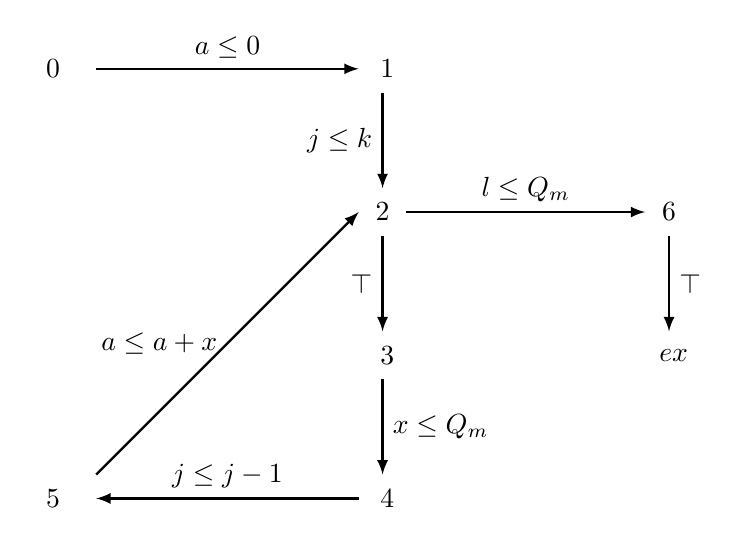
\begin{tikzpicture}[scale=\textwidth/20cm,samples=200]
  \draw[] (-7, 10) circle (0pt) node{{ $0$}};
  \draw[] (0, 10) circle (0pt) node{{ $1$}};
  \draw[] (0, 7) circle (0pt) node{\textbf{$2$}};
  \draw[] (0, 4) circle (0pt) node{{ $3$}};
  \draw[] (0, 1) circle (0pt) node{{ $4$}};
  \draw[] (-7, 1) circle (0pt) node{{ $5$}};
  % Counter Variables
  \draw[] (6, 7) circle (0pt) node {\textbf{$6$}};
  \draw[] (6, 4) circle (0pt) node {{ $ex$}};
  %
  % Control Flow Edges:
  \draw[ thick, -latex] (-6, 10)  -- node [above] {$a \leq 0$}(-0.5, 10);
  \draw[ thick, -latex] (0, 9.5)  -- node [left] {$j \leq k$} (0, 7.5) ;
  \draw[ thick, -latex] (0, 6.5)  -- node [left] {$\top$}  (0, 4.5);
  \draw[ thick, -latex] (0, 3.5)  -- node [right] {$x \leq Q_m$} (0, 1.5) ;
  \draw[ thick, -latex] (-0.5, 1)  -- node [above] {$j \leq j - 1$} (-6, 1) ;
  \draw[ thick, -latex] (-6, 1.5)  -- node [left] {$a \leq a + x$} (-0.5, 7)  ;
  \draw[ thick, -latex] (0.5, 7)  -- node [above] {$l \leq Q_m$}  (5.5, 7);
  \draw[ thick, -latex] (6, 6.5)  -- node [right] {$\top$} (6, 4.5) ;
  \end{tikzpicture}
  \caption{}
    \end{centering}
    \end{subfigure}
    \begin{subfigure}{.45\textwidth}
      \begin{centering}
    %   \todo{abstract-cfg for two round}
    \begin{tikzpicture}[scale=\textwidth/20cm,samples=200]
    \draw[] (-10, 10) circle (0pt) node{{ $0: 1$}};
    \draw[] (0, 10) circle (0pt) node{{ $1: 1$}};
    \draw[] (0, 7) circle (0pt) node{\textbf{$2: k$}};
    \draw[] (0, 4) circle (0pt) node{{ $3: k$}};
    \draw[] (0, 1) circle (0pt) node{{ $4: k$}};
    \draw[] (-10, 1) circle (0pt) node{{ $5: k$}};
    % Counter Variables
    \draw[] (6, 7) circle (0pt) node {\textbf{$6: 1$}};
    \draw[] (6, 4) circle (0pt) node {{ $ex: 1$}};
    %
    % Control Flow Edges:
  \draw[ thick, -latex] (-8, 10)  -- node [above] {$a \leq 0$}(-1.5, 10);
  \draw[ thick, -latex] (0, 9.5)  -- node [left] {$j \leq k$} (0, 7.5) ;
  \draw[ thick, -latex] (0, 6.5)  -- node [left] {$\top$}  (0, 4.5);
  \draw[ thick, -latex] (0, 3.5)  -- node [right] {$x \leq Q_m$} (0, 1.5) ;
  \draw[ thick, -latex] (-1.5, 1)  -- node [above] {$j \leq j - 1$} (-8, 1) ;
  \draw[ thick, -latex] (-8, 1.5)  -- node [left] {$a \leq a + x$} (-1.5, 7)  ;
  \draw[ thick, -latex] (1.5, 7)  -- node [above] {$l \leq Q_m$}  (4.5, 7);
  \draw[ thick, -latex] (6, 6.5)  -- node [right] {$\top$} (6, 4.5) ;
    \end{tikzpicture}
    \caption{}
      \end{centering}
      \end{subfigure}
    \caption{(a) The same $\kw{towRounds(k)}$ program as Figure~\ref{fig:twoRounds_example}
    (b) The abstract control flow graph for $\kw{towRounds(k)}$  (c) The abstract control flow graph with the reachability bound for $\kw{towRounds(k)}$.}
    \vspace{-0.5cm}
    \label{fig:abscfg_tworound}
  \end{figure}
\end{example}
%
% In order to estimate weight for every vertex in $\progV(c)$,
%  I first show how to compute the reachability bound for every label in $c$
%  % (i.e., every vertex in $\absV(c)$)
%  (i.e., the $\absW(c)$), 
%  then show how to compute the weight for every vertex in $\progV(c)$.
%  \\
%  Through the edges in $\absG(c)$, which correspond to $c$'s abstract transition between labels,

%  \wq{In order to estimate weight for every vertex in the static analysis dependency graph($\progV(c)$), I want to find out the upper bound on 
%  the number of times the labeled command (uniquely associated with a vertex in $\progV(c)$) may be executed when running the program.
%  This information can be obtained by computing the reachability bound for every vertice in the abstract control flow graph ($\absW(c)$), because
%  the vertices in the two graph share the same unique label, the line number.  I can easily show that the reachability bound on one vertex of the actract control flow graph is also the upper bound for the corresponding vertex in the static analysis dependency graph, both vertices share the same unique line number.}



%   I perform the symbolic reachability bound anaysis on the abstract control flow graph, 
%  through the edges in $\absG(c)$, which correspond to $c$'s abstract transition between labels.
%  I infer the invariant for every variable, and compute the transition closure for every abstract transition. By solving the closure
%  with the invariants of variables involved in this closure for every transition, I compute
%  the symbolic reachability bound of every commands corresponding to this transition.
%  \\
%  Specifically in four steps, Variable Modification Tracking, Local Bounds Computation,
%  the symbolic reachability bound of every commands corresponding to this transition. Specifically, this analysis can be performed in four steps:
%   Variable Modification Tracking, Local Bounds Computation,
%  Invariant Inference and Closure Generation, and Reachability Bound Computation,
{In order to estimate weight for every vertex in the static analysis dependency graph($\progV(c)$), I want to find out the upper bound on 
the number of times the labeled command (uniquely associated with a vertex in $\progV(c)$) may be executed when running the program.
This information can be obtained by computing the reachability bound for every vertex in the abstract control flow graph ($\absW(c)$), because
the vertices in the two graph share the same unique label, the line number.  I can easily show that the reachability bound on one vertex of the abstract control flow graph is also the upper bound for the corresponding vertex in the static analysis dependency graph, both vertices share the same unique line number.}


 I perform the symbolic reachability bound analysis on the abstract control flow graph, 
through the edges in $\absG(c)$, which correspond to $c$'s abstract transition between labels.
 I infer the invariant for every variable, and compute the transition closure for every abstract transition. By solving the closure
with the invariants of variables involved in this closure for every transition, I compute
the symbolic reachability bound of every commands corresponding to this transition. Specifically, this analysis can be performed in four steps:
 Variable Modification Tracking, Local Bounds Computation,
Invariant Inference and Closure Generation, and Reachability Bound Computation,
% 
%  I present the details of invariant, closure generation, and reachability bound computation as follows.
with details as follows.
%
%
\paragraph*{Variable Modification Tracking}
Identify the abstract events where each variable is increased, decreased and reset:
\\
$\inc: \mathcal{VAR} \to \mathcal{P}(\absevent) $
the set of the abstract events where the variable increase.
\\
$\inc(x) = \{(\absevent, c) | \absevent = (l, l', x' \leq x + v)\}$
\\
$\reset: \mathcal{VAR} \to \mathcal{P}(\absevent) $
The set of the abstract events where the variable is reset.
\\
$\dec: \mathcal{VAR} \to \mathcal{P}(\absevent) $
The set of abstract events where the variable decrease.
% \\
% $\dec(x) = \{(\absevent, c) | \absevent = (l, l', x' \leq x - v)\}$
\\
$Incr(v) \triangleq \sum\limits_{(\absevent, c) \in \inc(v)}\{\absclr(\absevent) \times v\}$
%
\paragraph*{Local Bounds}
Given a program $c$ with its abstract control flow graph 
$\absG(c) = (\absV, \absE)$
\\
Local Bounds Computation:
$\locbound: \absevent \to \mathcal{VAR} \cup \constdom$.
%
\[ 
\begin{array}{ll}
  \locbound(\absevent) \triangleq 1 
  & \absevent \notin SCC(\absG(c))
  \\
  \locbound(\absevent) \triangleq (x, v) 
  & \absevent \in SCC(\absG(c)) \land \absevent \in \dec(x) \land  \absevent = (\_, \_ , x' \leq x - v) \\
  \locbound(\absevent) \triangleq (x, \max(\dec(x))) 
  & \absevent \in SCC(\absG(c)) \land 
  \absevent  \notin \bigcup_{x \in \mathcal{VAR}} \dec(x)
  \land \absevent \notin SCC(\absG(c) \setminus \dec(x)) 
\end{array}
  \]
  The first case is straightforward. Since variable's visiting time outside of any while loop is at most 1, I do not need to analyze the visiting times of every node in the graph from phase 1.
  The second and third step is guaranteed by the \emph{Discussion on Soundness} in Section 4 of \cite{sinn2017complexity}.
  Then soundness proof is in Lemma~\ref{lem:local_bound_sound} in Appendix~\ref{apdx:reachability_soundness}.
%
\paragraph*{Invariant Inference and Closure Generation }
Then, computing the bound invariants for variables and the transition closures for abstract events:
\\ 
$ \varinvar: \mathcal{VAR} \cup \constdom \to EXPR(\constdom)$
\\
$\absclr: \absevent \to EXPR(\constdom)$
\\
Then, the symbolic invariant for each variable 
as well as the symbolic transition closure for each transition is calculated as follows:
\[ 
\begin{array}{lll}
  \varinvar(x) & \triangleq c & c \in \constdom \\
  \varinvar(x) & \triangleq Incr(v) + \max(\{\varinvar(a) + c | (t, a, c) \in \reset(x)\}) & c \notin \constdom
\end{array}
\]
%
\begin{defn}
  \label{def:transition_closure_base}
\[ 
\begin{array}{lll}
  \absclr(\absevent) 
  & \triangleq x / v & \\ 
  & \locbound(\absevent) = (x, v) \in \constdom \times \mathbb{N} & \\
  \absclr(\absevent) 
  & \triangleq (Incr(x) + 
  \sum\limits_{(\absevent', y, v') \in \reset(x)}
  \absclr(\absevent') \times \max(\varinvar(y) + v', 0) ) / v & \\
  & \locbound(\absevent) = (x, v) \land x \notin \constdom & 
\end{array}
  \]
\end{defn}
%
\paragraph*{Improved Variable Modification Tracking}
Instead of just identifying the abstract events where each variable is reset,
this improvement identifies the chain of the events where a given variable is reset by the 
variables of the abstract events through the chain.
\\
$\resetchain: \mathcal{VAR} \to \mathcal{P}(\mathcal{P}(\absevent)) $
The set of the chain of abstract events where the variable is reset through the chain.
% \\
% $Incr(v) \triangleq \sum\limits_{(\absevent, c) \in \inc(v)}\{\absclr(\absevent) \times v\}$
%
\paragraph*{Improved Invariant Inference and Closure Generation}
Then, computing the bound invariants for variables and the transition closures for abstract events:
\\ 
$ \varinvar: \mathcal{VAR} \cup \constdom \to EXPR(\constdom)$
\\
$\absclr: \absevent \to EXPR(\constdom)$
\\
Then, the symbolic invariant for each variable 
as well as the symbolic transition closure for each transition is calculated as follows:
\[ 
\begin{array}{lll}
  \varinvar(x) & \triangleq c & c \in \constdom \\
  \varinvar(x) & \triangleq Incr(v) + \max(\{\varinvar(a) + c | (t, a, c) \in \reset(x)\}) & c \notin \constdom
\end{array}
\]
%
\begin{defn}
  \label{def:transition_closure}
\[ 
\begin{array}{lll}
  \absclr(\absevent) 
  & \triangleq x / v & \\ 
  & \locbound(\absevent) = (x, v) \in \constdom \times \mathbb{N} & \\
  \absclr(\absevent) 
  & \triangleq \Big(
    \sum\limits_{y \in \{ y ~|~ 
    ch \in \resetchain(x), (l_1, x, y, v, l_2) \in ch \} } Incr(x) & \\
    & \quad + 
  \sum\limits_{ch \in \resetchain(x)}
  \big( \min\limits_{\absevent' \in ch}({\absclr(\absevent')}) \times 
  \max(\varinvar(y) + \sum\limits_{(l_1, x, y, v, l_2) \in ch } v, 0)\big) \Big) / v & \\
  & \locbound(\absevent) = (x, v) \land x \notin \constdom & 
\end{array}
  \]
\end{defn}
  %
% \paragraph*{Adding the Reachability Bounds for Every Vertex in the Data-Control Flow Graph}
% Updating the weight of every vertex in the $\progG(c) = (\progV, \progE, \progW, \progF)$ for program $c$ generated from phase 1. 
% For every $x^l \in \progV$, find the abstract event $\absevent \in \absflow(c)$ of the form $(l, \_, \_)$, updating the $\progW(x^l) $ by the transition closure of this event.
% \\
$
\progW(x^l) 
  \triangleq \absclr(\absevent)
$
\paragraph*{Reachability Bound Computation}
Through the transition closure computed above, 
The weight of every label in 
% Then I update 
the program $c$'s abstract control flow graph,
$\absG(c) =(\absV, \absE, \absW)$
is 
computed as the maximum over all the abstract events $\absevent \in \absE$ heading out from this vertex, formally as follows.
% by annotating each vertex with a symbolic weight. 
% This weight corresponds to 
%reachability bounds of
\\
$\absW 
\triangleq \left\{ (l, w) \in \mathbb{N} \times EXPR(\constdom) | w = \max\limits_{\absevent = (l, \_, \_)} \{ \absclr(\absevent)\} \right\}$.
% \\
\paragraph*{Example}
 I perform the symbolic reachability bound analysis on the abstract control flow graph as follows. 
 I would like to generate the closure of every edge, which is an equality relation between variables.  Solving this closure gives us the reachability bound for this edge. With all the bound for all the edges in the abstract control flow graph, I can calculate the weight for every vertex in this graph. For example, I show the closure generated for the edge 
$(4, j < j - 1, 5)$, 
$\absclr(4, 5) = \varinvar(j)$. The invariant for variable $j$, $\varinvar(j)$ used here is 
$\varinvar(j) = k * \absclr(1, 2)$, which is generated by all the difference constraints involving $j$ in the graph. Notice the $k$ in $\varinvar(j)$ comes from considering both difference constraint $j<=k$ from edge (1,2) and $j<=j-1$ from (4,5), which intuitively reflects the while loop whose counter is set to $k$ at the beginning and decreases by 1 at each iteration. 
With all the closures for all the edges of the abstract control flow graph, I can solve them to obtains the reachability bound of every edge.  I decide the weight for every vertex in the abstract control flow graph by using the bound of the edges which head out from this vertex, by taking the max of the bound from these involving edges. For instance,   
By the constraint on the edge $(4, j \leq j - 1, 5)$, I get bound $k$ for this edge.
Then, I assign vertex $4$ by reachability bound $k$, as in Figure~\ref{fig:abscfg_tworound}(c). 
Another interesting vertex is $2$, which has more than one edge heading out from it, $(2, \top, 3)$ and $(2,\top, 6)$. For the weight for vertex $2$, I choose the max between the bound $k$ from $(2,\top, 3)$ and $1$ from $(2,\top, 6)$.
The same way for the rest weights' computation.
 I use $\absW(c)$ for the set of weights I just computed 
for each label in the abstract control flow graph of $c$.
% Still looking at the two-round example as in Figure~\ref{fig:adapfun_tworound}(b) where 
% each label $l$ is added with a weight by $absW$.
% This weight represents the  maximum reaching times of this location $l$, in the other word, 
% the estimated maximum visiting times of the command labeled with $l$.
% For example, looking at the vertex $1$,
% by analysis steps, since it isn't in any SCC, it's estimated reachability bound is computed as $1$.
% However, for the vertex $4$ which is involved in an SCC, the reachability bound is inferred in another way.
% By the constraint on the edge $4, j \leq j - 1, 5$,
% I first infer its local bound as variable $j$.
% Then by solving the invariant for variable $j$,
% I infer the value bound for $j$, which is $k$.
% Then the reachability bound for this abstract transition, (i.e., edge $4, j \leq j - 1, 5$) 
% is computed as $k$ as well through Definition~\ref{def:abs_trace}.
% In this abstract control flow graph, every vertex is a label,
% corresponding to a label command in the program.
% Each directed 
% edge represents an abstract transition 
% between two control locations, 
% i.e., the labels of two commands (we call the labels also control location and they refer to the same thing), 
% where the second labeled command will be executed after execution of the command with first label.
% For example, the edge $0, a \leq 0, 1$ on the top, represents,
% from location $0$, the command 
% $\clabel{\assign{a}{0}}^0$ is executed with next continuation location $1$,
% where the 
% command $\clabel{\assign{j}{k}}^1$ will be executed next.
% The constraint $a \leq 0$ is generated by abstracting from the assignment command $\assign{a}{0}$,
% representing that value of $a$ is less than or equals to $0$ after 
% location $0$ before executing command at line $1$.
%
The same way for the rest weights' computation.
\paragraph{Vertex Weight Computation}
% The weight for each vertex in $\progV(c)$ is computed as follows,
Then I compute the weight for each vertex in $\progV(c)$,
% as a set of pairs $\progW(c) \in \mathcal{P}(\mathcal{LV} \times \mathcal{LV} \times EXPR(\constdom))$ 
as a set of pairs 
% is the set of pairs 
% The weight for each vertex in $\progV(c)$ is computed 
mapping each $x^l \in \progV(c)$ to a symbolic expression over $\constdom$. Since symbolic expression 
over $\constdom$ is a subset of arithmetic expressions,
we use $\mathcal{A}_{in}$ denotes the arithmetic expression 
over $\mathcal{N}$ and input variable and $\progW(c) \in \mathcal{P}(\mathcal{LV} \times \mathcal{A}_{in})$ 
as follows,
\highlight{
% :
% \\
 \[\progW(c) \triangleq
   \left\{ (x^l, w) 
  %  \in  \mathcal{LV} \times \expr
\mid
x^l \in \progV(c) \land (l, w) \in \absW(c)
\right\}.
\]
}
%
% Since 
 I prove that this 
% symbolic expression is the upper bound for $x^l$'s 
symbolic expression for $x^l \in \progV(c)$ is a sound upper bound of 
the weight for the same vertex $x^l$ in Program's execution-based dependency graph in Appendix~\ref{apdx:reachability_soundness}.
The maximum visiting times of $x^l$ over all execution traces of $c$ in Appendix~\ref{apdx:reachability_soundness}. 
%
\begin{thm}[Soundness of the Reachability Bounds Estimation]
  \label{thm:addweight_soundness}
Given a program ${c}$ with its program-based dependency graph 
$\progG = (\progV, \progE, \progW, \progF)$,
$\traceG = (\traceV, \traceE, \traceW, \traceF)$, I have:
%
\[
\forall (x^l, w_{t}) \in \traceW,
(x^l, w_{p}) \in \progW, \vtrace \in \mathcal{T} \sthat 
% \lvar_c \sthat  
%  \vcounter(\vtrace') l ~ \middle\vert~
% \forall \vtrace \in \mathcal{T} \sthat  
\config{{c}, \trace} \to^{*} \config{\eskip, \trace\tracecat\vtrace'} 
\land 
\config{w_{p}, \trace} \earrow v
\implies
% \right\} 
\leq 
w_{t}(\trace) \leq v
\]
\end{thm}
\paragraph*{Example}
Now let's 
% where I goes 
go back to the Program-Based Dependency Graph which I aim to build for approximating the 
Execution-Based Dependency graph for two-round example, as in
Figure~\ref{fig:twoRounds_example}(c).
%
%  looking at the two-round example,
%  as in  where we
% each vertex in 
%  $l$ is added with a weight by $absW$.
% This weight represents the  maximum reaching times of this location $l$, in the other word, 
% the estimated maximum visiting times of the command labeled with $l$.
% For example, looking at the vertex $1$,
% by analysis steps, since it isn't in any SCC, it's estimated reachability bound is computed as $1$.
% However, for the vertex $4$ which is involved in an SCC, the reachability bound is inferred in another way.
% By the constraint on the edge $4, j \leq j - 1, 5$,
% I first infer its local bound as variable $j$.
% Then by solving the invariant for variable $j$,
Every vertex from $\progV(c)$ in this graph corresponds to a labeled variable, for example $a^5$,
and this label $5$ is also a vertex $5$ in the abstract control flow graph in Figure~\ref{fig:abscfg_tworound}(b).
%
% I infer the value bound for $j$, which is $k$.
% Then the reachability bound for this abstract transition, (i.e., edge $4, j \leq j - 1, 5$) 
Then, it is straight forward, 
that the reachability bound for the label $5$, 
is also the maximum visiting times bound of the labeled variable $a^5$.
% is computed as $k$ as well through Definition~\ref{def:abs_trace}.
% In this abstract control flow graph, every vertex is a label,
% corresponding to a label command in the program.
So, I estimate the visiting time for  labeled variable $a^5$ in Program-Based Dependency Graph in Figrue~\ref{fig:abscfg_tworound}(c) as $k$ as well.
%
The same way for the rest weights' computation.
%
\subsection{Data Dependency Relation Analysis}
\label{sec:alg_edgegen}
% \wq{
   I show how to estimate the directed edges in the static analysis dependency graph.
 I develop a variant of data flow analysis, called Feasible Data-Flow Generation, which 
considers both the control flow and data flow and
is a sound approximation of the edges in the execution based dependency graph.
% }

% \wq{
  Also, worth to mention, I use the result of reaching definition on the abstract control flow graph in feasible 
data-flow generation to have a more precise approximation. Let us see a simple example, a program $ [x = 0]^{1}; [x=2]^{2};  [y = x+1]^{3}$. The standard data flow analysis 
tells us that both the labeled variable $x^{1}$ and $x${2} may flow to $y^{3}$, which will result in an unnecessary edge ($x^{1}, y^{3}$). The result of reaching definition 
can help us eliminate this kind of edge by telling us, at line $3$, only variable $x^{2}$ is reachable. 
% }


% In this step, through 
% % the vertices and edges in 
% $c$'s abstract contrl flow graph $\absG(c)$,
%  $\THESYSTEM$ performs a feasible data-flow analysis 
%  using the reachable definition algorithm,
% %  and then Then I generated the set of feasible data-flow between labeled variables based on that.
% and generates the 
% %set of 
% feasible data-flow relation between labeled variables.
% \\
%  By generating set of all the reachable variables at location of label $l$ in the program $c$.
% For every labelled variable $x^l$ in this set, 
% the value assigned to that variable
% in the assignment command associated to that label is reachable at the entry point of  executing the command of label $l$.
% \\
In the first step, 
it performs the standard reaching definition analysis given a program $c$, 
on 
% its every label $l$
every label in $\absV(c)$.  This step generates set of all the reachable variables at location of label $l$ in the program $c$.
The $\live(l, c)$ represent the analysis result, which is the set of 
reachable labeled variables in program $c$ at the location of label $l$.
For every labelled variable $x^l$ in this set, 
the value assigned to that variable
in the assignment command associated to that label is reachable at the entry point of  executing the command of label $l$.
% \\
% it performs the standard reaching definition analysis given a program $c$, on its every label $l$.
% \\
% Another operator \mathsf{blocks} 
The block, 
is either the command of the form of assignment, skip, or a test of the form of $[b]^{l}$, 
% and $block$ of program $c$ is 
denoted by $\mathsf{blocks}(c)$
the set of all the blocks 
in program $c$, where  $\mathsf{blocks}: \cdom \to \mathcal{P}(\cdom \cup \clabel{\bexpr}^{l})$.
Then it generates the set of feasible data-flow between labeled variables with detail in Definition~\ref{def:feasible_flowsto}, 
based on $\live(l, c)$ for every label in a program $c$ and its blocks $\mathsf{blocks}$.
\\
The details are as follows.
%
% Performing a feasible data-flow analysis through the reachable definition algorithm. 
%  By generating set of all the reachable variables at location of label $l$ in the program $c$.
% For every labelled variable $x^l$ in this set, 
% the value assigned to that variable
% in the assignment command associated to that label is reachable at the entry point of  executing the command of label $l$.
% \paragraph{Generate CFG}
%  \begin{def}
%   \label{def:init_label}
%   Define $\mathsf{init}$: Command -> label, which returns the initial label of the statement. 
% \[
%  \begin{array}{ll}
%     init([x := e]^{l})  & = l  \\
%      init([x := q(e)]^{l})  & = l \\
%      init([skip]^{l})  & = l \\
%      init([if [b]^l then C_1 else C_2]^{l})  & = l \\
%      init([while [b]^l do C]^{l})  & = l \\
%      init(C_1 ; C_2)  & = init(C_1) \\
%  \end{array}
%  \]
% \end{def}
%   Define $\mathsf{final}$: Command -> Powerset(label), which returns the final labels of the statement. 
%  \[
%  \begin{array}{ll}
%     final([x := e]^{l})  & = \{l\}  \\
%      final([x := q(e)]^{l})  & = \{l\}  \\
%      final([skip]^{l})  & = \{l\} \\
%      final([if [b]^l then C_1 else C_2]^{l})  & = final(C_1) \cup final(C_2) \\
%      final([while [b]^l do C]^{l})  & = \{l\} \footnote{while terminates after b evaluates to false} \\
%      final(C_1 ; C_2)  & =  final(C_2) \\
%  \end{array}
%  \]
% \paragraph*{Blocks and Defs}
%  Define block B to be either the command of the form of assignment, skip, or test of the form of $[b]^{l}$.\\
%  Define $\mathsf{blocks}$ : command -> Powerset(Block)
%  \[
%  \begin{array}{ll}
%     blocks([x := e]^{l})  & = \{[x := e]^{l}\}  \\
%      block([x := q(e)]^{l})  & = \{[x := q(e)]^{l}\}  \\
%      blocks([skip]^{l})  & = \{[skip]^{l}\} \\
%      blocks([if [b]^l then C_1 else C_2]^{l})  & = {[b]^{l}} \cup blocks(C_1) \cup blocks(C_2) \\
%      blocks([while [b]^l do C]^{l})  & = \{[b]^{l}\} \cup blocks(C) \\
%      blocks(C_1 ; C_2)  & = blocks(C_1) \cup  blocks(C_2) \\
%  \end{array}
%  \]
%  Define $\mathsf{labels}$ to get the labels of blocks.
%  \[
%    labels(C) = \{l | [B]^{l} \in blocks(C) \}
%  \]  

% The control flow graph is generated by edges between labels. Define $\mathsf{flow}$: command -> P (label $\times$ label ).

% \[
%  \begin{array}{ll}
%     flow([x := e]^{l})  & = \emptyset  \\
%      flow([x := q(e)]^{l})  & = \emptyset  \\
%      flow([skip]^{l})  & = \emptyset \\
%      flow([if [b]^l then C_1 else C_2)  & =  flow(C_1) \cup flow(C_2)\cup \{(l, init(C_1)) , (l, init(C_2)) \} \\
%      flow([while [b]^l do C)  & =  flow(C) \cup \{(l, init(C)) \} \cup \{(l', l)| l' \in final(C) \} \\
%      flow(C_1 ; C_2)  & = flow(C_1) \cup  flow(C_2) \cup \{ (l,init(C_2)) | l \in final(C_1) \} \\
%  \end{array}
%  \]
 
 \paragraph{Reaching definition analysis}
 \todo{extend and formalize}
%  Define block B to be either the command of the form of assignment, skip, or test of the form of $[b]^{l}$.\\
%  Define $\mathsf{blocks}$ : command -> Powerset(Block)
A block  is either the command of the form of assignment, skip, or test of the form of $[b]^{l}$.\\
The operator $\mathsf{blk} : \cdom \to blocks$ gives all the blocks in program $c$.
\\
%  \[
%  \begin{array}{ll}
%     blocks([x := e]^{l})  & = \{[x := e]^{l}\}  \\
%      block([x := q(e)]^{l})  & = \{[x := q(e)]^{l}\}  \\
%      blocks([skip]^{l})  & = \{[skip]^{l}\} \\
%      blocks([if [b]^l then C_1 else C_2]^{l})  & = {[b]^{l}} \cup blocks(C_1) \cup blocks(C_2) \\
%      blocks([while [b]^l do C]^{l})  & = \{[b]^{l}\} \cup blocks(C) \\
%      blocks(C_1 ; C_2)  & = blocks(C_1) \cup  blocks(C_2) \\
%  \end{array}
%  \]
 Set $?$ to be undefined:
 \\
%  $label^{?}$ is label $\cup \{?\}$.\\
%  Define $\mathsf{kill}$: $blocks \to \mathcal{P}(\mathcal{VAR} \times LABEL \cup \{?\})$, which produces the set of labelled variables of assignment destroyed by the block.
The operator $\mathsf{kill}$: $blocks \to \mathcal{P}(\mathcal{VAR} \times \ldom \cup \{?\})$ produces the set of labelled variables of assignment destroyed by the block.
 \\
  % Define $\mathsf{gen}$: $blocks \to \mathcal{P}(\mathcal{VAR} \times LABEL \cup \{?\})$, which generates the set of labelled variables generated by the block.
  The operator $\mathsf{gen}$: $blocks \to \mathcal{P}(\mathcal{VAR} \times \ldom \cup \{?\})$ generates the set of labelled variables generated by the block.
  \\
  % Define $defs(x)(c): \mathcal{VAR} \to LABEL$, gives all the labels where assigns value to variable x in the target program $c$. 
  % The operator  $defs(c): \mathcal{VAR} \to \ldom$ gives all the labels where assigns value to variable in $c$. 
%  \[
%  \begin{array}{ll}
%     kill([x := e]^{l})  & = \{ (x, ?) \} \cup \{ (x, l') | l' \in defs(x) \} \\
%      kill([x := q(e)]^{l})  & = \{ (x, ?) \} \cup \{ (x, l') | l' \in defs(x) \}  \\
%      kill([skip]^{l})  & = \emptyset \\
%      kill([ [b]^l ]^{l})  & =  \emptyset
%  \end{array}
%  ~~
%   \begin{array}{ll}
%       gen([x := e]^{l})  & = \{ (x, l) \}  \\
%      gen([x := q(e)]^{l})  & = \{ (x, l) \}  \\
%      gen([skip]^{l})  & = \emptyset \\
%      gen([ [b]^l ]^{l})  & =  \emptyset 
%  \end{array}
%  \]
%  Define $in(l)$, $out(l)$: LABEL$ \to \mathcal{VAR} \times LABEL \cup \{?\}$ for every block in program $c$ is computed as follows,
%  \[
%  \begin{array}{lll}
%     in(l)  & = \{ (x, ?) | x^l \in \lvar_c \land  l = \absinit(c) \}  
%     \cup \{ out(l')|  | (l',\_, l) \in \absE \land  l \neq \absinit(c)\}  \\
%      out(l)  & =  gen(B^{l}) \cup \{ in(l) \setminus kill(B^l)  \} & B^l \in blocks(c)   
%  \end{array}
%  \]
%  computing $in(l)$ and $out(l)$ for every $B^l \in blocks(c) $, and repeating these two step
% until the $in(l)$ and $out(l)$ are stabilized for every $B^l \in blocks(c) $
%  I use $\live_{in}(l,c)$ and $\live_{out}(l, c)$ denote the stabilized results for the command of label $l$ in program $c$. 
%  Define $defs(x)(c): \mathcal{VAR} \to LABEL$, gives all the labels where assigns value to variable x in the target program $c$.
% Define $defs(x)(c): \mathcal{VAR} \to \ldom$, gives all the labels where assigns value to variable x in the target program $c$.
% \\
%  Define $in(l)$, $out(l)$: $ \ldom \to \mathcal{VAR} \times LABEL \cup \{?\}$ for every block in program $c$ is computed as follows,
The operator  $in(l)$, $out(l)$: $ \ldom \to \mathcal{LV} \cup \{?\}$ for every block in program $c$ is defined as follows,
 \[
 \begin{array}{ll}
    % in(l)  & = \{ (x, ?) | x^l \in \lvar_c \land  l = \absinit(c) \}  
    in(l)  & = \{ x^{?} | x^l \in \lvar_c \land  l = \absinit(c) \}  
    \cup \{ out(l')|  | (l',\_, l) \in \absE(c) \land  l \neq \absinit(c)\}  \\
     out(l)  & =  gen(B^{l}) \cup \{ in(l) \setminus kill(B^l)  \}  
 \end{array}
 \]
computing $in(l)$ and $out(l)$ for every $B^l \in blocks(c) $, and repeating these two steps
until the $in(l)$ and $out(l)$ are stabilized for every $B^l \in blocks(c) $
%  I use $\live_{in}(l,c)$ and $\live_{out}(l, c)$ denote the stabilized results for the command of label $l$ in program $c$. 
 I use $\live(l,c)$ to represent 
% $\live_{in}(l,c)$ in the other part of the paper.
denote the stabilized result of $in(l)$ at label $l$ in program $c$. 
% The $\live_{in}(l,c)$ and $\live_{out}(l, c)$ is computed by the Standard worklist algorithm. (For simplicity, I use $\live(l,c)$ to represent $\live_{in}(l,c)$ in the other part of the paper.}
\\
% The $\live_{in}(l,c)$ and $\live_{out}(l, c)$ 
The stabilized $in(l)$ and $out(l)$ for program $c$, as well as $\live(l, c)$,
is computed by the standard worklist algorithm with detail as below. 
% For simplicity, I use $\live(l,c)$ to represent $\live_{in}(l,c)$ in the other part of the paper.
\begin{enumerate}
    \item initial in[l]=out[l]=$\emptyset$
    \item initial in[entry label] = $\emptyset$
    \item initialize a work queue, contains all the blocks in C
    \item while |W| != 0 \\
         pop l in W\\
          old = out[l]\\
          in(l) =  out(l') where $(l',\_, l) \in \absE(c)$\\
           out(l) = gen($b^l$) $\cup$ (in(l) - kill($b^l$) ) where $b^l$ in $\mathsf{blk}(c)$   \\
          if (old != out(l)) W= W $\cup$ \{l'| (l,l') in $(l',\_, l) \in \absE(c)$\}\\
          end while
\end{enumerate}
%
% computing $in(l)$ and $out(l)$ for every $B^l \in blocks(c) $, and repeating these two step
% until the $in(l)$ and $out(l)$ are stabilized for every $B^l \in blocks(c) $
%  I use $\live_{in}(l,c)$ and $\live_{out}(l, c)$ denote the stabilized results for the command of label $l$ in program $c$. 
% The $\live_{in}(l,c)$ and $\live_{out}(l, c)$ is computed by the Standard worklist algorithm. (For simplicity, I use $\live(l,c)$ to represent $\live_{in}(l,c)$ in the other part of the paper.
%%
\paragraph{Feasible Data-Flow Generation}
by using the results of Reaching definition analysis results, specifically $\live(l, c)$ for every label in a program $c$, I refine the vertices and edges in the $\absG$ graph 
by generating the set of feasible data-flow between labeled variables as follows,
%
%   \[
%  \begin{array}{ll}
%     dcdg([x := e]^{l})  & = \{ (y^i, x^l) | y \in VAR(e) \land (y,i) \in \live_{in}(l) \}  \\
%      dcdg([x := q(e)]^{l})  & = \{ (y^i, x^l) | y \in VAR(e) \land (y,i) \in \live_{in}(l) \}  \\
%      dcdg([skip]^{l})  & = \emptyset \\
%      dcdg([if [b]^l then C_1 else C_2)  & =  dcdg(c_1) \cup dcdg(c_2)\\ & \cup \{(x^i,y^j) | x \in VAR(b) \land (x,i) \in \live_{in}(l) \land ([y = \_]^j) \in blocks(c_1) \} \\
%      &\cup \{(x^i,y^j) | x \in VAR(b) \land (x,i) \in \live_{in}(l) \land ([y = \_]^j) \in blocks(c_2) \} \\
%      dcdg([while [b]^l do c)  & =  dcdg(c) \cup \{(x^i,y^j) | x \in VAR(b) \land (x,i) \in \live_{in}(l) \land ([y = \_]^j) \in blocks(C) \} \\
%      dcdg(c_1 ;c_2)  & = dcdg(c_1) \cup  dcdg(c_2) \\
%  \end{array}
%  \]
%
\begin{defn}[Feasible Data-Flow]
  \label{def:feasible_flowsto}
  Given a program $c$ and two labeled variables $x^i, y^j$  in this program, 
  $\flowsto(x^i, y^j, c)$ is 
    {\footnotesize
    \[
   \begin{array}{ll}
    \flowsto(x^i, y^j, \clabel{\assign{x}{\expr}}{}^l)  & \triangleq (x^i, y^j) \in \{ (y^i, x^l) | y \in \mathsf{FV}(\expr) 
    % \land (y,i) \in \live(l, \clabel{\assign{x}{\expr}}^l) \}  \\
    \land y^i \in \live(l, \clabel{\assign{x}{\expr}}^l) \}  \\
    \flowsto(x^i, y^j, \clabel{\assign{x}{\query(\qexpr)}}{}^l)  & \triangleq (x^i, y^j) \in \{ (y^i, x^l) | y \in \mathsf{FV}(\qexpr) 
    % \land (y,i) \in \live(l,\clabel{\assign{x}{\query(\qexpr)}}^l) \}  \\
    \land y^i \in \live(l,\clabel{\assign{x}{\query(\qexpr)}}^l) \}  \\
    \flowsto(x^i, y^j, [\eskip]^{l})  & = \emptyset \\
    \flowsto(x^i, y^j, \eif ([b]^l, c_1, c_2))  & \triangleq \flowsto(x^i, y^j, c_1) \lor \flowsto(x^i, y^j, c_2) \\ 
        & \lor (x^i, y^j) \in
       \{(x^i,y^j) | x \in \mathsf{FV}(b) \land 
      %  (x,i) 
      x^i \in \live(l, \eif ([b]^l, c_1, c_2)) \land  y^j \in \lvar(c_1) \\
    %   ([y = \_]^j) \in \mathsf{blk}(c_1) \} \\
       &\lor (x^i, y^j) \in \{(x^i,y^j) | x \in \mathsf{FV}(b) \land 
      %  (x,i) 
      x^i\in \live(l, \eif ([b]^l, c_1, c_2))  \land  y^j \in \lvar(c_2) \\
    %   \land ([y = \_]^j) \in \mathsf{blk}(c_2) \} \\
       \flowsto(x^i, y^j, \ewhile [b]^l \edo c_w)  & \triangleq  \flowsto(x^i, y^j, c_w)  \lor
       \\ & 
       (x^i, y^j) \in  \{(x^i,y^j) | x \in \mathsf{FV}(b) \land 
      %  (x,i) 
      x^i \in \live(l,   \ewhile [b]^l \edo c_w) \land  y^j \in \lvar(c_w) \\
    %   ([y = \_]^j) \in \mathsf{blk}(c_w) \} \\
       \flowsto(x^i, y^j, c_1 ;c_2)  & \triangleq \flowsto(x^i, y^j, c_1) \lor \flowsto(x^i, y^j, c_2) \\
   \end{array}
   \]
   }
   \end{defn}
%
This \emph{Feasible Data-Flow} relation is a sound approximation 
of the \emph{variable may-Dependency} relation over labeled variables for every program.
The soundness is proved
in Appendix~\ref{apdx:flowsto_soundness}.
%
\paragraph*{Edges Estimation}
Then I define the estimated directed edges
% for each vertex in $\progV(c)$,
between vertices in $\progV(c)$,
as a set of pairs 
% $\progW(c) \in \mathcal{P}(\mathcal{LV} \times \mathcal{LV} \times EXPR(\constdom))$ 
$\progE(c) \in \mathcal{P}(\in \mathcal{LV} \times \mathcal{LV})$
% is the set of pairs 
% The weight for each vertex in $\progV(c)$ is computed 
indicating a directed edge from the first vertex to the second one in each pair
as follows,
\highlight{
  \[
    \progE(c) \triangleq 
    \left\{ 
    ({x}_1^{i}, {x}_2^{j}) \in \mathcal{LV} \times \mathcal{LV}
    ~ \middle\vert ~
    \begin{array}{l}
      {x}_1^{i}, {x}_2^{j} \in \progV(c)
    \land
      % \\
      \exists n \in \mathbb{N}, z_1^{r_1}, \cdots, z_n^{r_n} \in \lvar_{{c}} \sthat  
      n \geq 0 \land
      \\
      \flowsto(x^i,  z_1^{r_1}, c) 
      \land \cdots \land \flowsto(z_n^{r_n}, y^j, c) 
    \end{array}
    \right\}
    \]
}
This estimated directed edge set $\progE(c)$ is a sound approximation of the 
edge set in $c$'s execution-based dependency graph, which is proved 
in Appendix~\ref{apdx:adapt_soundness}.
%  \begin{defn}[Feasible Data-Flow]
%   \label{def:feasible_flowsto}
%     {\footnotesize
%     \[
%    \begin{array}{ll}
%       dcdg(\clabel{\assign{x}{\expr}}{}^l)  & = \{ (y^i, x^l) | y \in FV(e) \land (y,i) \in \live_{in}(l, \clabel{\assign{x}{\expr}}^l) \}  \\
%        dcdg(\clabel{\assign{x}{\query(\qexpr)}}{}^l)  & = \{ (y^i, x^l) | y \in FV(e) \land (y,i) \in \live_{in}(l,\clabel{\assign{x}{\query(\qexpr)}}^l) \}  \\
%        dcdg([\eskip]^{l})  & = \emptyset \\
%        dcdg([\eif [b]^l \ethen c_1 \eelse c_2)  & =  dcdg(c_1) \cup dcdg(c_2)\\ & \cup 
%        \{(x^i,y^j) | x \in FV(b) \land (x,i) \in \live_{in}(l) \land ([y = \_]^j) \in blocks(c_1) \} \\
%        &\cup \{(x^i,y^j) | x \in FV(b) \land (x,i) \in \live_{in}(l) \land ([y = \_]^j) \in blocks(c_2) \} \\
%        dcdg([\ewhile [b]^l \edo c)  & =  dcdg(c) \cup \{(x^i,y^j) | x \in FV(b) \land (x,i) \in \live_{in}(l) \land ([y = \_]^j) \in blocks(C) \} \\
%        dcdg(c_1 ;c_2)  & = dcdg(c_1) \cup  dcdg(c_2) \\
%    \end{array}
%    \]
%    }
%    \end{defn}
%    For any two labeled variables $x^i, y^j$ in a program $c$, 
%   %  it is easy to see that there is a one-on-one correspondence between 
%   %  $\flowsto$ relation of the two variables, and the $dcdg$ analysis result on $c$.
%   I use $\flowsto()$ denote if they have a feasible data-flow relation in Definition~\ref{def:flowsto}.
%    \begin{defn}[Feasible Data-Flow ($\flowsto$)]
%    \label{def:flowsto}
%    \[
%    \forall c \in \cdom, x^i, y^j \in \lvar_c \sthat  
%    \flowsto(x^i, y^j, c) \iff (x^i, y^j) \in dcdg(c)
%    \]
%    \end{defn}
  %  This soundness is proved in Proof~\ref{pf:rd_soundness} in Appendix~\ref{apdx:rd_soundness}.
  %  For any two labeled variables in a program $c$, it is easy to see that there is a one-on-one correspondence between 
  %  $\flowsto$ relation of the two variables, and the $dcdg$ analysis result on $c$.
  %  \begin{thm}[Soundness of the Feasible Data-Flow Analysis]
  %  \label{thm:rd_soundness}
  %  \[
  %  \forall c \in \cdom, x^i, y^j \in \lvar_c \sthat  
  %  \flowsto(x^i, y^j, c) \iff (x^i, y^j) \in dcdg(c)
  %  \]
  %  \end{thm}
  %  This soundness is proved in Proof~\ref{pf:rd_soundness} in Appendix~\ref{apdx:rd_soundness}.
  \paragraph*{Example}
% Still looking at the Figure~\ref{fig:adapfun_tworound}(c), 
% and taking the edge $(l^6, a^5)$ for example.
% By $\flowsto(l^6, a^5, c)$, I can see $a$ is used directly in the query expression $\chi[k]*a$,
% in the assignment command $\clabel{\assign{l}{\query(\chi[k]*a)}}^l$,
% i.e., $a \in FV(\chi[k]*a)$.
% Also, from the Reaching definition analysis, I know $a^5 \in \live(6, two-round)$.
% Then I have $\flowsto(l^6, a^5, c)$ and construct the edge $(l^6, a^5)$.
% And same way for constructing the rest edges.
%
The edge $(l^6, a^5)$ in Figure~\ref{fig:twoRounds_example}(c) is constructed by this definition.
% and take  for example.
By $\flowsto(l^6, a^5, c)$, I can see $a$ is used directly in the query expression $\chi[k]*a$,
in the assignment command $\clabel{\assign{l}{\query(\chi[k]*a)}}^l$,
i.e., $a \in FV(\chi[k]*a)$.
Also, from the reaching definition analysis, I know $a^5 \in \live(6, \kw{twoRounds(k)})$.
Then I have $\flowsto(l^6, a^5, c)$ and construct the edge $(l^6, a^5)$.
And the same way for constructing the rest edges. Also, the edge $(x^3,j^5)$ in the same graph represents the control flow, 
caught by the $\flowsto$ relation.

% Still looking at the Figure~3(c) in main paper, 
% and taking the edge $(l^6, a^5)$ for example.
% By $\flowsto(l^6, a^5, c)$, I can see $a$ is used directly in the query expression $\chi[k]*a$,
% in the assignment command $\clabel{\assign{l}{\query(\chi[k]*a)}}^l$,
% i.e., $a \in FV(\chi[k]*a)$.
% Also, from the Reaching definition analysis, I know $a^5 \in \live(6, two-round)$.
% Then I have $\flowsto(l^6, a^5, c)$ and construct the edge $(l^6, a^5)$.
% And same way for constructing the rest edges. Also, the edge $(x^3,j^5)$ in the same graph represents the control flow, caught by our $\flowsto$ relation.
%


% \section{Syntax of {\Arel}}
% The syntax is shown as follows,
\[
\begin{array}{llll}
\mbox{Arithmetic Operators} 
& \oplus_a & ::= & + ~|~ - ~|~ \times 
%
~|~ \div ~|~ \max ~|~ \min\\  
% \mbox{Unary Operators} 
% & \oplus_a & ::= & + ~|~ - ~|~ \times 
% %
% ~|~ \div \\  
\mbox{Boolean Operators} 
& \oplus_b & ::= & \lor ~|~ \land
\\
%
\mbox{Relational Operators} 
& \sim & ::= & < ~|~ \leq ~|~ == 
\\  
%
\mbox{Label} 
& l & \in & \mathbb{N} \cup \{\lin, \lex\} 
\\ 
%
\mbox{Arithmetic Expression} 
& \aexpr & ::= & 
n ~|~ {x} ~|~ \aexpr \oplus_a \aexpr  
% \\
% &  &  & 
 ~|~ \elog \aexpr  ~|~ \esign \aexpr
\\
%
\mbox{Boolean Expression} & \bexpr & ::= & 
%
\etrue ~|~ \efalse  ~|~ \neg \bexpr
 ~|~ \bexpr \oplus_b \bexpr
%
~|~ \aexpr \sim \aexpr 
\\
%
\mbox{Expression} & \expr & ::= & v ~|~ \aexpr ~|~ \bexpr ~|~ [\expr, \dots, \expr]
\\  
%
\mbox{Value} 
& v & ::= & { n ~|~ \etrue ~|~ \efalse ~|~ [] ~|~ [v, \dots, v]}  
\\
%
\highlight{\mbox{Query Expression}  }
& {\qexpr} & ::= 
& \highlight{ \qval ~|~ \aexpr ~|~ \qexpr \oplus_a \qexpr ~|~ \chi[\aexpr]}
\\
%
\highlight{\mbox{Query Value} }& \qval & ::= 
& \highlight{n ~|~ \chi[n] ~|~ \qval \oplus_a  \qval ~|~ n \oplus_a  \chi[n]
    ~|~ \chi[n] \oplus_a  n}
    \\
% &&& \text{\mg{I don’t think this is what I want. Isn’t $\chi[n+1]$ a query value?}}\\
% &&& \text{\mg{What about $\chi[i] + \chi[i] + \chi[i]$? They are not in the grammar}}
% \\
% &&& \text{\jl{ $\chi[i] + \chi[i] + \chi[i]$ and $\chi[n+1]$ are both expressions, they will be evaluated to a value 
% }}
% \\%
\mbox{Labeled Command} 
& {c} & ::= &   [\assign {{x}}{ {\expr}}]^{l} ~|~  \highlight{[\assign {{x} } {{\query(\qexpr)}}]^{l}}
~|~ {\ewhile [ \bexpr ]^{l} \edo {c} }
\\
&&&
~|~ {c};{c}  
~|~ \eif([\bexpr]{}^l , {c}, {c}) 
~|~ [\eskip]^l
\\ 
\mbox{Event} 
& \event & ::= & 
    ({x}, l, v, \bullet) ~|~ ({x}, l, v, \qval)  ~~~~~~~~~~~ \mbox{Assignment Event} \\
&&& ~|~(\bexpr, l, v, \bullet)   ~~~~~~~~~~~~~~~~~~~~~~~~~~~~~~~~~~ \mbox{Testing Event}
\\
\mbox{Trace} & \trace
& ::= & [] ~|~ \trace :: \event
\\
\end{array}
\]
% \[
% \begin{array}{llll}
% \mbox{Arithmetic Operators} 
% & \oplus_a & ::= & + ~|~ - ~|~ \times 
% %
% ~|~ \div ~|~ \max ~|~ \min\\  
% % ~|~ \div \\  
% \mbox{Boolean Operators} 
% & \oplus_b & ::= & \lor ~|~ \land
% \\
% %
% \mbox{Relational Operators} 
% & \sim & ::= & < ~|~ \leq ~|~ == 
% \\  
% %
% \mbox{Arithmetic Expression} 
% & \aexpr & ::= & 
% n ~|~ {x} ~|~ \aexpr \oplus_a \aexpr  
%  ~|~ \elog \aexpr  ~|~ \esign \aexpr
% \\
% %
% \mbox{Boolean Expression} & \bexpr & ::= & 
% %
% \etrue ~|~ \efalse  ~|~ \neg \bexpr
%  ~|~ \bexpr \oplus_b \bexpr
% %
% ~|~ \aexpr \sim \aexpr 
% \\
% %
% \mbox{Expression} & \expr & ::= & v ~|~ \aexpr ~|~ \bexpr ~|~ [\expr, \dots, \expr] ~|~ \highlight{\fname}
% \\  
% %
% \mbox{Value} 
% & v & ::= & { n ~|~ \etrue ~|~ \efalse ~|~ [] ~|~ [v, \dots, v]}  
% \\ 
% &&&
% \highlight
% {
% ~|~ (x_0, x_1, \ldots, x_n) := c
% }
% \\
% %
% \highlight{\mbox{Query Expression}} 
% & {\qexpr} & ::= 
% & \highlight{ \qval ~|~ \aexpr ~|~ \qexpr \oplus_a \qexpr ~|~ \chi[\aexpr]} 
% \\
% %
% \mbox{Query Value} & \qval & ::= 
% & \highlight{n ~|~ \chi[n] ~|~ \qval \oplus_a  \qval ~|~ n \oplus_a  \chi[n]
%     ~|~ \chi[n] \oplus_a  n}
% \\
% % \\%
% \mbox{Label} 
% & l & ::= & (n \in \mathbb{N} \cup \{\lin, \lex\}) ~|~ (l, n)
% \\ 
% %
% \mbox{Labeled Command} 
% & {c} & ::= &  
% \clabel{\assign{x}{\expr}}^l 
% ~|~ \clabel{\assign{x}{\query(\qexpr)}}^l
% ~|~  \clabel{\eskip}^l
% ~|~ \ewhile \clabel{\bexpr}^{l} \edo {c}
% ~|~ \eif(\clabel{\bexpr}^{l} , {c}, {c}) 
% \\ 
% &&&
% \highlight
% {
% ~|~ \clabel{\efun}^l: \fname (x_0, x_1, \ldots, x_n) := c
% ~|~ \clabel{\assign{x}{\ecall(x, e_1, \ldots, e_n)}}^l
% }
% ~|~ {c};{c}  
% \\ 
% % \\
% \mbox{Event} 
% & \event & ::= & 
%     ({x}, l, v, \bullet) ~|~ ({x}, l, v, \qval) ~|~ (\fname, l, v, \qval)  ~~~~~~~~~~~ \mbox{Assignment Event} \\
% &&& ~|~(\bexpr, l, v, \bullet)   ~~~~~~~~~~~~~~~~~~~~~~~~~~~~~~~~~~ \mbox{Testing Event}
% \\
% % &&& \text{\mg{I think it would be better to use quadruples for events, where the}}\\
% % &&& \text{\mg{first element is either a variable or a boolean expression and }}\\
% % &&& \text{\mg{the last is either a query value or some default value $\bullet$}}\\
% %
% % \mbox{Trace} & \trace
% % & ::= & \cdot | \trace \cdot \event | \trace \tracecat \trace 
% % \\
% %
% % \mbox{Trace} & \trace
% % & ::= & [] ~|~ \event:: \trace ~|~ \trace \tracecat \trace  \\
% \mbox{Trace} & \trace
% & ::= & [] ~|~ \trace :: \event\\
% % &&& \text{\mg{I don't understand why you need both :: and ++ as constructors.}}\\
% % &&& \text{\jl{Because append is to the left but we are adding element to the left in the OS}}\\
% % &&& \text{\jl{I was too sticky to the convention, it is a good idea to append to the left and just use $::$}}
% % %
% % \mbox{Event Signature} & \sig
% % & ::= & (x, l, n) | (x, l, n, \query) | (b, l, n)
% % \\
% % %
% \end{array}
% \]
For clarity, the following notations are used to represent the set of corresponding terms:
\[
\begin{array}{lll}
\mathcal{VAR} & : & \mbox{Set of Variables}  
\\ 
%
\mathcal{VAL} & : & \mbox{Set of Values} 
\\ 
%
\mathcal{QVAL} & : & \mbox{Set of Query Values} 
\\ 
%
\cdom & : & \mbox{Set of Commands} 
\\ 
%
\mathcal{LV} & : & \mbox{Set of Labeled Variables}
\\
%
\eventset  & : & \mbox{Set of Events}  
\\
%
\eventset^{\asn}  & : & \mbox{Set of Assignment Events}  
\\
%
\eventset^{\test}  & : & \mbox{Set of Testing Events}  
\\
%
\ldom  & : & \mbox{Set of Labels}  
\\
%%
\mathcal{VAL}  & : & \mbox{Set of Labeled Variables}  
\\
%%
\dbdom  & : & \mbox{{Set of Databases}} 
\\
%
{\mathcal{T}} & : & \mbox{Set of Traces}
\\
%
% \qdom = {[-1,1]} & : & \mbox{{Domain of Query Results}}\\
\qdom & : & \mbox{{Domain of Query Results}}\\
% &&\text{\mg{I don't think you need to hard code [-1,1] here}}\\
\end{array}
\]
\paragraph*{Standard Expression}
The expressions are either the standard one or the extended one.
A standard expression is
% can be 
either a standard arithmetic expression or a boolean expression, or a list of expressions.
An arithmetic expression can be a constant $n$ denoting integer, a variable $x$ from some countable set $\mathcal{VAR}$, binary operation $\oplus_a$ such as addition, product, subtraction, etc, over arithmetic expressions, and also log and sign operation. 
%
A boolean expression can be either {\tt true} or {\tt false}, basic boolean connectives such as logical negation, logical and and or denoted by $\oplus_b$, and basic comparison $sym$ between arithmetic expressions, e.g., $\leq,=,<,$ etc.
Additionally, I also introduce list in expression.
Our language supports primitives for queries, 
where a specific query is specified by a query expression $\qexpr$. 
A query expression contains the necessary information for a query request, for example, 
$\chi[\aexpr]$ represents the values at a certain index $\aexpr$ in a row $\chi$ of the database. 
Query expressions combine access to the database with other expressions, 
for example, $\chi[3] + 5$ represents a query which asks the value from the column 3 of each database raw $\chi$, adds 5 to each of these values, 
and then computes the average of these values.
\paragraph*{Query Expression}
The key extension is
%  language supports 
the primitive for queries, where a specific query is specified by a query expression $\qexpr$. 
A query expression contains the necessary information for a query request, 
for example, $\chi[\qexpr]$ represents the values at a certain index $\qexpr$ in a row $\chi$ of the database. 
When this expression is encapsulated by the symbol $\query$,
 $ \query(\chi[\qexpr]) $ computes the average value at certain index over each row of the database as follows,
 \[
  \query(\chi[\qexpr]) = \frac{1}{n}\sum\limits_{i = 0}^{n}\chi_i[\qexpr]
  \]
Query expressions combine access to the database with other expressions, 
for example, 
$\chi[3] + 5$ represents a query that asks the value from column 3 of each database raw $\chi$, 
adds 5 to each of these values, and then computes the average of these values as follows, where $n$ is 
data base $\chi$'s number of raw.
%
\[
  \query(\chi[3] + 5) = \frac{1}{n}\sum\limits_{i = 0}^{n}\chi_i[3] + 5
  \]

% the expression also includes the special variable $\chi$ representing a row of the database, and access to values at a certain index in $\chi$, as $\chi[\aexpr]$. Additionally, list over expressions is supported and $[]$ stands for the empty list. The access to elements in the list can be achieved through $x[\aexpr]$ when variable $x$ is referred to a list. The value $v$ now contains the natural number $n$, the boolean primitives $\etrue$ and $\efalse$, the special row $\chi$ and access to it $\chi[v]$, the empty list $[]$ and non-empty list $[v, \dots, v]$.
% 
% Another extension is the inter-procedure call and function definition.
% In the function define command $\clabel{\efun}^l: \fname (x_0, x_1, \ldots, x_n) := c$,
% the function body $c$ is assigned to the function of name $\fname$, $x_1, \ldots, x_n$ is the function
% arguments and the first element $x_0$ in the arguments is the return variable.
% We only support the first-order function definition and function call. 

% %
\paragraph*{Labeled Command}
 A labeled command $c$ is just a command with a label --- I assume that labels are unique, so that they can help to identify uniquely every subexpression. 
%  I have $\eskip$, assignment $\assign{x}{\expr}$, the composition of two commands $c;c$, an if statement $\eif(\bexpr, c, c)$, a while statement  $\ewhile \bexpr \edo {c} $.
 The main novelty of the syntax is the query request command $\assign{x}{\query(\qexpr)}$. 
 For instance, if a data analyst wants to ask a simple linear query which returns the first element of the row, 
 they can simply use the command $ \assign{x}{\query(\chi[1])}$ in their data analysis program.
%  \wq{Shall I distinguish command and labeled command, they are now both $c$. }
%  \jl{I'm not sure, I don't want to programmer to add the label when writing the program. The label is just added by us for analysis. but I'm worried it is too complicate if use two notations for command and labeled command }
%
% \[
% \begin{array}{llll}
% \mbox{Label} 
% & l & \in & \mathbb{N} \cup \{in, ex\} \\
% \mbox{Labeled Commands} 
% & {c} & ::= &   [\assign {{x}}{ {\expr}}]^{l} ~|~  [\assign {{x} } {{\query(\qexpr)}}]^{l}
% ~|~ {\ewhile [ \bexpr ]^{l} \edo {c} }
%  \\
%  &&&
% ~|~ {c};{c}  
% ~|~ \eif([\bexpr]{}^l , {c}, {c}) 
% ~|~ [\eskip]^l 
% \end{array}
% \]
\paragraph*{Labeled Variables}
The labeled variables and assigned variables are set of variables annotated by a label. 
We use  
%$\mathcal{LVAR} = \mathcal{VAR} \times \mathcal{L} $ 
$\mathcal{LV}$ represents the universe of all the labeled variables and 
$\avar_c \in \mathcal{P}(\mathcal{VAR} \times \mathbb{N}) \subset \mathcal{LV}$ and 
$\lvar_c \in \mathcal{P}(\mathcal{VAR} \times \mathcal{L}) \subseteq \mathcal{LV}$,
represents the the set of assigned variables and labeled variables for a labeled command $c$,
defined in Definition~\ref{def:lvar} and \ref{def:avar}.
%
% \\
$FV: \expr \to \mathcal{P}(\mathcal{VAR})$, computes the set of free variables in an expression. To be precise,
$FV(\aexpr)$, $FV(\bexpr)$ and $FV(\qexpr)$ represent the set of free variables in arithmetic
expression $\aexpr$, boolean expression $\bexpr$ and query expression $\qexpr$ respectively.
Labeled variables in $c$ is the set of assigned variables and all the free variables
showing up in $c$ with a default label $in$. 
The free variables
showing up in $c$, which aren't defined before be used, are actually the input variables of this program.
%
%
\begin{defn}[Assigned Variables (
% $\avar_{c} \subseteq \mathcal{VAR} \times \mathbb{N}$ or 
$\avar : \cdom \to \mathcal{P}(\mathcal{VAR} \times \mathbb{N})$)]
% labelled Variables 
% (
% % $\lvar_{c} \subseteq \mathcal{VAR} \times \mathbb{N}$ or 
% $\lvar : \cdom \to \mathcal{P}(\mathcal{VAR} \times \mathcal{L})$
\label{def:avar}
$$ \avar_{c} \triangleq
  \left\{
  \begin{array}{ll}
      \{{x}^l\}                   
      & {c} = [{\assign x e}]^{l} 
      \\
      \{{x}^l\}                   
      & {c} = [{\assign x \query(\qexpr)}]^{l} 
      \\
      \avar_{{c_1}} \cup \avar_{{c_2}}  
      & {c} = {c_1};{c_2}
      \\
      \avar_{{c}} \cup \avar_{{c_2}} 
      & {c} =\eif([\bexpr]^{l}, c_1, c_2) 
      \\
      \avar_{{c}'}
      & {c}   = \ewhile ([\bexpr]^{l}, {c}')
\end{array}
\right.
$$
\end{defn}
%
%
\begin{defn}[labelled Variables 
(
% $\lvar_{c} \subseteq \mathcal{VAR} \times \mathbb{N}$ or 
$\lvar : \cdom \to \mathcal{P}(\mathcal{LV})$]
\label{def:lvar}
$$
  \lvar_{c} \triangleq
  \left\{
  \begin{array}{ll}
      \{{x}^l\} \cup FV(\expr)^{in}                  
      & {c} = [{\assign x e}]^{l} 
      \\
      \{{x}^l\}   \cup FV(\qexpr)^{in}                
      & {c} = [{\assign x \query(\qexpr)}]^{l} 
      \\
      \lvar_{{c_1}} \cup \lvar_{{c_2}}  
      & {c} = {c_1};{c_2}
      \\
      \lvar_{{c}} \cup \lvar_{{c_2}} \cup FV(\bexpr)^{in}
      & {c} =\eif([\bexpr]^{l}, c_1, c_2) 
      \\
      \lvar_{{c}'} \cup FV(\bexpr)^{in}
      & {c}   = \ewhile ([\bexpr]^{l}, {c}')
\end{array}
\right.
$$
\end{defn}
%
%
%
% is a subset of the program's assigned variables, where every variable in this set is assigned by a query in the program.
% \mg{The set of query variables of a program is the set of variables set to the result of a query in the program.}\\
% In the same way, in order to 
\paragraph*{Query Variables}
Distinctively, a key definition for the extension of the query primitives 
is the set of query variables for a program $c$.
This definition is the key point to track the query requests in the Following full-spectrum adaptivity analysis.
% track the I also defined the set of query variables for a program $c$.
It is defined as the set of variables,
which are assigned by the result of a query request in the program formally in Definition~\ref{def:qvar}.
% \mg{In the next definition, why do you call it a vector? It seems that you define it as a set.}\\
% \jl{fixed}\\
%
% \begin{defn}[Query Variables ($\qvar_{c} \subseteq \mathcal{VAR} \times \mathbb{N}$)].
  % \\
\begin{defn}[Query Variables ($\qvar: \cdom \to \mathcal{P}(\mathcal{LV})$)] 
  \label{def:qvar}
Given a program $c$, its query variables 
% \mg{it seems you are missing the $_c$ subscript. Also, this is a minor point but I don't think it is a good idea to use a subscript, cannot you just use $\qvar(c)$.}
$\qvar(c)$ is the set of variables set to the result of a query in the program.
% \jl{fixed}
It is defined as follows:
{
$$
  % \qvar_{{c}} \triangleq
  \qvar(c) \triangleq
  \left\{
  \begin{array}{ll}
      % \{\}                  
      % & {c} = [{\assign x e}]^{(l, w)} 
      % \\
      % \{{x}^l\}                  
      % & {c} = [{\assign x \query(\qexpr)}]^{(l, w)} 
      % \\
      % \qvar_{{c_1}} \cup \qvar_{{c_2}}  
      % & {c} = {c_1};{c_2}
      % \\
      % \qvar_{{c_1}} \cup \qvar_{{c_2}} 
      % & {c} =\eif([\bexpr]^{l}, c_1, c_2) 
      % \\
      % \qvar_{{c}'}
      % & {c}   = \ewhile ([\bexpr]^{l}, {c}')
      \{\}                  
      & {c} = [{\assign x \expr}]^{l} 
      \\
      \{{x}^l\}                  
      & {c} = [{\assign x \query(\qexpr)}]^{l} 
      \\
      \qvar(c_1) \cup \qvar(c_2)  
      & {c} = {c_1};{c_2}
      \\
      \qvar(c_1) \cup \qvar(c_2) 
      & {c} =\eif([\bexpr]^{l}, c_1, c_2) 
      \\
      \qvar(c')
      & {c}   = \ewhile ([\bexpr]^{l}, {c}')
\end{array}
\right.
$$
}
\end{defn}
%
It is easy to see that a program $c$'s query variables is a subset of 
its labeled variables, $\qvar(c) \subseteq \lvar(c)$.
%
% \mg{In this definition as well as in others, I have the impression that you assume that the labelled variables are unique in the program. For example, it would not make sense to assign a query to the same labelled variable over and over. If this is the case, I need to make this very explicit in the paper.}
% \jl{TODO}
%
Every labeled variable in a program is unique, formally as follows with proof in Appendix~\ref{apdx:lemma_sec123}.
\begin{lem}[Uniqueness of the Labeled Variables]
  \label{lem:lvar_unique}
  For every program $c \in \cdom$ and every two labeled variables such that
  $x^i, y^j \in \lvar(c)$, then $x^i \neq y^j$.
  \[
    \forall c \in \cdom, x^i, y^j \in \mathcal{L} \sthat x^i, y^j \in \lvar(c)\implies x^i \neq y^j.
    \]
\end{lem}

\highlight{\paragraph*{Improvements through Examples}
It is expressive in two following aspects.
\begin{itemize}
  \item \textbf{Improvements from Standard While Language}
  \\
  It also extends the standard while language with query requests. 
  The general data analysis program with query requests on data  are supported in this {\tt Query While} language.
  The program can access the database through a special  interface $\chi$ encapsulated by the identifier $\query$ (for example the program below) in the new language.
  \[
    {\assign{x}{20}};
    \assign{y}{\query(\chi[2])};
    \ewhile (x < 100) \edo 
    \{
      \assign{x}{x + 1};
      \assign{y}{\query(\chi[x]*\chi[n])};
      \}\}
    \] 
%
    \item \textbf{Improvements from Previous Works}
  \\
This {\tt Query While} language is also more expressive than the language designed in previous works.
The previous language only supports the data analysis with constant number of loop iterations.
Comparing to it, in the new language design,
the general data analysis program with non-deterministic loop iterations
(for example the program below as shown in Section~\ref{sec:prework-language})
is supported.
\[
  {\assign{x}{20}};
  \assign{y}{40};
  \ewhile (x < y) \edo 
  \{
    \assign{x}{x + 1};
    \assign{y}{y - 2};
    \}\}
  \] 
Previous work does not support data analysis program with user inputs, which is supported in the new language as well.
\end{itemize}
}

% \clearpage
% \section{Metatheory of {\Arel}}
% \input{chapters/arel/appendix/theory}


% \stoplist[appendix]{lof}

% % \chapter*{Glossary of Terms}
\label{glossary}
\begin{longtable}{r p{0.6\textwidth}}
    \textbf{\textit{Complicated Term}}: & Make sure to define anything that you allude to in the text\\
    \textbf{\textit{Parameter}}: & Description of the parameter. This is not the same as the List of Symbols. \\
\end{longtable}
% \end{appendices}
%%%%%%%%%%%%%%%%%%%%%%%%%%%%%%%%%%%%%%%%%%%%%%%%%%%%%%%%%%%%%%%%%%%%
% The back matter



%%%%%%%%%%%%%%%%%%%%%%%%%%%%%%%%%%%%%%%%%%%%%%%%%%%%%%%%%%%%%%%%%%%%
%%%% LIST OF JOURNAL ABBREVIATIONS	
% If you don't write the journal names out in full in the bibliography then you need a list of journal abbreviations
% \chapter*{List of Journal Abbreviations}
% I have included a list of common journals that are used in Biostatistics. Make sure that your .bib file abbreviations match what is here. - HG 2018
\begin{center}
\begin{longtable}{lp{0.56\textwidth}}
  Am J Epidemiol \dotfill & American Journal of Epidemiology \\
  Am J Public Health \dotfill & American Journal of Public Health \\
  Am Stat \dotfill & The American Statistician \\
  Ann Intern Med \dotfill & Annals of Internal Medicine \\
  Ann Stat \dotfill & The Annals of Statistics \\
  Arch Intern Med \dotfill & Archives of Internal Medicine \\
  BMJ \dotfill & The British Medical Journal \\
  Can J Stat \dotfill & The Canadian Journal of Statistics \\
  IEEE Trans Automat Contr \dotfill & Institute of Electrical and Electronics Engineers Transactions on Automatic Control \\
  JAMA \dotfill & Journal of the American Medical Association \\
  JASA \dotfill & Journal of the American Statistical Association \\
  J R Stat Soc Ser B \dotfill & Journal of the Royal Statistical Society. Series B (Statistical Methodology) \\
  J R Stat Soc Ser C \dotfill & Journal of the Royal Statistical Society. Series C (Applied Statistics) \\
  J Stat Softw \dotfill & The Journal of Statistical Software \\
  N Engl J Med \dotfill & New England Journal of Medicine \\
  Stat Med \dotfill & Statistics in Medicine 
\end{longtable}
\end{center}


%%%%%%%%%%%%%%%%%%%%%%%%%%%%%%%%%%%%%%%%%%%%%%%%%%%%%%%%%%%%%%%%%%%%
%%%% 	BIBLIOGRAPHY	
% The bibliography itself can be single spaced with at least one extra space between items

% 1.8.1 Formatting the bibliography
% Include a complete bibliography at the end of the work. Arrange the bibliography alphabetically by the last name of the primary author. You may single-space citations, but leave one line of space between citations. If you use an article style format, where each chapter has its own separate bibliography, you must also include a cumulative bibliography at the end of the work.
% Verify any other requirements for formatting the bibliography at the end of the work. Certain disciplines/departments may require an alternate arrangement to the bibliography, for example, separating primary and secondary sources and then arranging each alphabetically by last name of author.

\newpage
\singlespace
\Urlmuskip=0mu plus 1mu\relax % Don't let the website links get all funky and break the page margins
\bibliographystyle{apa-good} % technically, you need APA. This style file adds the URL to websites and the date accessed. NOTE: Mendeley API does not put the "date accessed" into the .bib file, so you may want to export directly - HG 2018
\bibliography{main.bib} % keep this on, or you will get warnings about undefined citations


%%%%%%%%%%%%%%%%%%%%%%%%%%%%%%%%%%%%%%%%%%%%%%%%%%%%%%%%%%%%%%%%%%%%
%%%%% CURRICULUM VITAE 
% Finally you must include your cv.  You can do that whatever way you like including by formatting it in a totally different program.

% If you would like to grab it from some other source then be sure the page numbering is consecutive with the end of the bibliography and be sure it appears on the table of contents by adding a line such as
% \addcontentsline{toc}{chapter}{Curriculum Vitae}

\chapter*{Curriculum Vitae}
% \thispagestyle{empty}
\begin{large}
\begin{center}
\textbf{Jiawen Liu, MA}\\ 
\today\\
\end{center}
\end{large}

\setlength{\columnsep}{1.5in}
\begin{multicols}{1}{
\begin{center}{
21 Overlook Ridge Ter, unit 527 \\ Revere, MA 02151 \\ (716) 429 6041 \\ \hyperlink{mailto:personaladdress@gmail.com}{jiawenliu18@gmail.com}\\
Work office \\Boston University \\ Boston, MA 02118 \\\hyperlink{mailto:buemail@bu.edu}{jiawenl@bu.edu}\\}
\end{center}}
\end{multicols}

\subsection*{Academic Training:}
\begin{tabular}{p{0.22\textwidth}p{0.7\textwidth}}
12/2023\small(expected) &  Ph.D. Boston University, Boston, MA; Computer Science\\
06/2017  & B.A. Central University of Economics and Finance, Haidian, Beijing; Department of Information Science. \\
\end{tabular}

\subsection*{Doctoral Research:}
\begin{tabular}{p{0.2\textwidth}p{0.72\textwidth}}
\textbf{Title}: & Program-based Analysis For Quantitative Properties \\
\textbf{Thesis advisor}: & Marco Gaboardi, PhD\\
\textbf{Defense date}: & December 3, 2021 \\
\textbf{Summary}: & Reasoning about quantitative properties of programs has great potential in program optimization and program security. This dissertation exploits the program-based analysis to reason about quantitative properties in different areas.
\\
\end{tabular}

\subsection*{Original, Peer Reviewed Publications (newest first):}
% Make sure to be consistent with your CV bibliographic info formatting
\begin{enumerate}
\item 
% \underline{Weihao Qu}, Marco Gaboardi, Deepak Garg. Relational cost analysis in functional-imperative setting. \emph{Journal of Functional Programming } 2022. \\(doi: 10.1017/S0956796821000071)
\item 
% \hyperlink{https://www.ncbi.nlm.nih.gov/pubmed/XXX}{XXX}.
% \item John Famous and Example Student. \emph{A special case of a well known conjecture}. Fancy Math. J. \textbf{46} no. 3 (2007), 473-490.
\end{enumerate}

\end{document}